\documentclass[a4paper,12pt,oneside]{book}
\usepackage[utf8]{inputenc}
\usepackage{textcomp}
\usepackage[parfill]{parskip} %Se necessatrio non indenta, ma inserisce spazio
\usepackage{graphicx}
\usepackage{hyperref}
\usepackage{amsmath} %To number equations

\usepackage{titling}
\newcommand{\subtitle}[1]{%
 \posttitle{%
 \par\end{center}
 \begin{center}\large#1\end{center}
 \vskip6.5em}%
}

\author{Andrea Onofri and Dario Sacco}
\date{Update: v. 0.9 (2021-10-06), compil. 2021-11-11}
\title{Experimental methods in agriculture}
\subtitle{}


%***************************************************************

%Specific RMarkdown
\usepackage{color}
\usepackage{fancyvrb}
\usepackage{longtable}
\usepackage{booktabs}
\providecommand{\tightlist}{%
  \setlength{\itemsep}{0pt}\setlength{\parskip}{0pt}}
\newcommand{\VerbBar}{|}
\newcommand{\VERB}{\Verb[commandchars=\\\{\}]}
\DefineVerbatimEnvironment{Highlighting}{Verbatim}{commandchars=\\\{\},fontsize=\small}
\usepackage{framed}
%\newenvironment{Shaded}{}{}
\newenvironment{Shaded}{\begin{snugshade}}{\end{snugshade}}
\definecolor{shadecolor}{RGB}{250,248,248}
\newcommand{\KeywordTok}[1]{#1}
\newcommand{\DataTypeTok}[1]{#1}
\newcommand{\DecValTok}[1]{#1}
\newcommand{\BaseNTok}[1]{#1}
\newcommand{\FloatTok}[1]{#1}
\newcommand{\ConstantTok}[1]{#1}
\newcommand{\CharTok}[1]{#1}
\newcommand{\SpecialCharTok}[1]{#1}
\newcommand{\StringTok}[1]{#1}
\newcommand{\VerbatimStringTok}[1]{#1}
\newcommand{\SpecialStringTok}[1]{#1}
\newcommand{\ImportTok}[1]{#1}
\newcommand{\CommentTok}[1]{#1}
\newcommand{\DocumentationTok}[1]{#1}
\newcommand{\AnnotationTok}[1]{#1}
\newcommand{\CommentVarTok}[1]{#1}
\newcommand{\OtherTok}[1]{#1}
\newcommand{\FunctionTok}[1]{#1}
\newcommand{\VariableTok}[1]{#1}
\newcommand{\ControlFlowTok}[1]{#1}
\newcommand{\OperatorTok}[1]{#1}
\newcommand{\BuiltInTok}[1]{#1}
\newcommand{\ExtensionTok}[1]{#1}
\newcommand{\PreprocessorTok}[1]{#1}
\newcommand{\AttributeTok}[1]{#1}
\newcommand{\RegionMarkerTok}[1]{#1}
\newcommand{\InformationTok}[1]{#1}
\newcommand{\WarningTok}[1]{#1}
\newcommand{\AlertTok}[1]{#1}
\newcommand{\ErrorTok}[1]{#1}
\newcommand{\NormalTok}[1]{#1}
% Redefine \includegraphics so that, unless explicit options are
% given, the image width will not exceed the width of the page.
% Images get their normal width if they fit onto the page, but
% are scaled down if they would overflow the margins.

\begin{document}

\maketitle
\tableofcontents

\hypertarget{introduction}{%
\chapter*{Introduction}\label{introduction}}
\addcontentsline{toc}{chapter}{Introduction}

This is the website for the book ``Experimental methods in agriculture'' and deals with the organisation of experiments and data analyses in agriculture and, more generally, in biology. Experiments are the key element to scientific progress and they need to be designed in a way that reliable data is produced. Once this fundamental requirement has been fullfilled, statistics can be used to summarise and explore the results, separating `signal' from `noise' and reaching appropriate conclusions.

In this book, we will try to give some essential information to support the adoption of good research practices, with particular reference to field experiments, which are used to compare, e.g., innovative genotypes, agronomic practices, herbicides and other weed control methods. We firmly believe that the advancement of cropping techniques should always be based on the evidence produced by scientifically sound experiments.

We will follow a `learn-by-doing' approach, making use of several examples and case studies, while keeping theory and maths at a minimum level; indeed, we are talking to agronomists and biologists and not to statisticians!

This website is (and will always be) free to use, and is licensed under the Creative Commons Attribution-NonCommercial-NoDerivs 3.0 License. It is written in RMarkdown with bookdown and it is rebuilt every now and then to incorporate corrections and updates. This is necessary, as R is a rapidly evolving language.

\hypertarget{aims}{%
\section*{Aims}\label{aims}}
\addcontentsline{toc}{section}{Aims}

This book is not written aiming at completeness, but it is finely tuned for a 6 ECTS introductory course in biometry, for master or PhD students. It is mainly aimed at building solid foundations for starting a job in the research field and, eventually, to be able to tackle more advanced statistical material.

\hypertarget{how-this-book-is-organised}{%
\section*{How this book is organised}\label{how-this-book-is-organised}}
\addcontentsline{toc}{section}{How this book is organised}

The first two Chapters deal with the experimental design and explain how to distinguish good from bad experiments. One key aspect is that we can never be sure that data are totally reliable and, thus, we assume that they are reliable whenever we can be reasonably sure that they were obtained by using reliable methods.

In Chapter 3 we learn how to describe the results, based on some simple stats, such as the mean, median, chi square value and Pearson correlation coefficient. In this chapter, we stick to the observed data, as if we were not interested in anything else. In chapter 4 we learn to see those observed data as the result of deterministic and stochastic processes, which we can describe by using statistical models.

In Chapters 5 and 6 we start recognising that the observed data is only one random sample from a wider universe of data and that we are mainly interested on that universe, as we want to use our experiment to draw general conclusions. Going from a sample to a population introduces a certain amount of uncertainty which we have to incorporate into our conclusions.

From Chapter 7 to Chapter 12 we deal with ANOVA, that is one of the most widely used techniques of data analysis, while the last two chapters deal with regression models.

Within each chapter, we usually start with some motivating examples so that you can see the bigger picture, and then dive into the details. In the final chapter, we provide exercises for each book section, which should help you you practice what you've learned.

\hypertarget{statistical-software}{%
\section*{Statistical software}\label{statistical-software}}
\addcontentsline{toc}{section}{Statistical software}

In this book, we will work through the examples using the R statistical software, together with the RStudio environment. We selected for a number of reasons: first of all we like it very much and we think that it is a pleasure to use it, once the initial difficulties have been overcame! Second, it is freeware, which is fundamental for the students. Third, in recent years the software skills of students in master programmes have notably increased and writing small chunks of code is no longer a problem for most of them. Last, but not least, we have seen that some experience with R is a very often required skill when applying for a job. Perhaps, we should say that we are very much indebted for the availability of those two wonderful pieces of free software.

R is characterised by a modular structure and its basic functionalities can be widely extended by a set of add-in packages. As this is mainly an introductory course, we decided, as long as possible, to stick to the main packages, which come with the basic R installation. However, we could not avoid the use of a few very important packages, which we will indicate later on. We should also mention that this book was built by using the `bookdown' package and it is hosted on the website blog `www.statforbiology.com,' which is built by using the `blogdown' package. We will not use these two packages during the course but we should mention that they were really useful.

We recognise that R has a steep learning curve and we will start from the very beginning, without assuming that the students have any preliminary knowledge, either about statistics, or about R.

\hypertarget{the-authors}{%
\section*{The authors}\label{the-authors}}
\addcontentsline{toc}{section}{The authors}

Andrea is Associate Professor at the Department of Agricultural, Food and Environmental Science, University of Perugia and he has taught `Experimental methods in Agriculture' since 2000. Dario was Associate Professors at the Department of Agricultural, Forest and Food Sciences, University of Torino; he used to teach `Experimental Methods in Agriculture' until 2020, when he suddenly died, far too early. Unfortunately, he could not see this book completed.

\hypertarget{science-and-pseudoscience}{%
\chapter{Science and pseudoscience}\label{science-and-pseudoscience}}

In the age of `information overload,' we have plenty of knowledge at our fingertips. We can `google' for a topic and our computer screen is filled with thousands of links, where we can find every piece of information we are looking for. However, one important question remains unanswered: which information is reliable and scientifically sound? We know by experience that the web is full of personal views, opinions, beliefs or, even worse, fake-news; we have nothing against opinions (although we would rather stay away from fake-news), but we need to be able to distinguish between subjective opinions and objective facts. Let's refer to the body of reliable and objective knowledge by using the term `science,' while all the rest is `non-science' or `pseudoscience'; the question is: ``How can we draw the line between science and pseudoscience?'' It is a relevant question in these days, isn't it?

A theory, in itself, is not necessarily science. It may be well-substantiated, it can incorporate good laws and/or equations, it may come either from a brilliant intuition or from a meticulous research work; it may come from a common man or from a very authoritative scientist\ldots{} it does not matter: theories do not necessarily represent objective facts. A few aphorisms can help us get to the point:

\begin{enumerate}
\def\labelenumi{\arabic{enumi}.}
\tightlist
\item
  Analogy cannot serve as proof (Pasteur)
\item
  The interest I have in believing a thing is not a proof of the existence of that thing (Voltaire)
\item
  A witty saying proves nothing (Voltaire)
\end{enumerate}

\hypertarget{science-needs-data}{%
\section{Science needs data}\label{science-needs-data}}

Theories need to proved. This fundamental innovation is usually attributed to Galileo Galilei (1564-1642), who is usually regarded as the founder of the scientific method, as summarised in Figure \ref{fig:figName11}.

\begin{figure}

{\centering 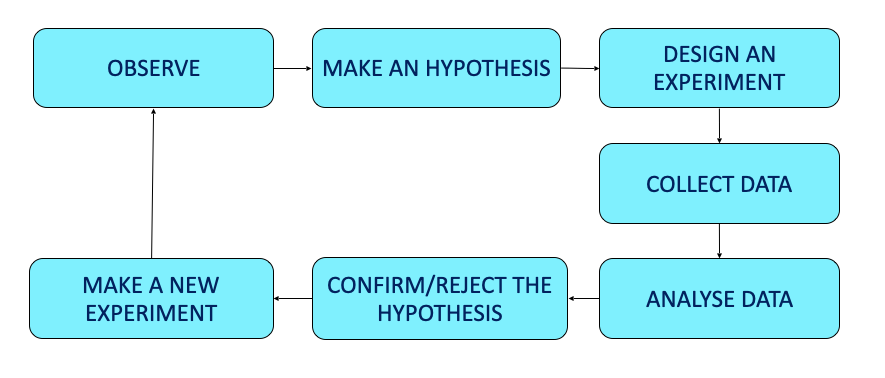
\includegraphics[width=0.75\linewidth]{_images/MSAMap} 

}

\caption{The steps to scientific method}\label{fig:figName11}
\end{figure}

Two aspects need attention:

\begin{enumerate}
\def\labelenumi{\arabic{enumi}.}
\tightlist
\item
  the fundamental role of scientific experiments, that produce data in support of pre-existing hypotheses (theories);
\item
  once a theory has been supported by the data, it is regarded as acceptable until new data disproves it and/or supports an alternative, more reliable or simpler, theory.
\end{enumerate}

Indeed, data is the most important ingredient of science; a very famous aphorism says ``In God we trust, all the others bring data.'' It is usually attributed to the American statistician, engineer and professor W. Edwards Deming (1900-1993), although it is also attributed to Robert W. Hayden. Trevor Hastie, Robert Tibshirani and Jerome Friedman, the authors of the famous book `The Elements of Statistical Learning,' mention that Professor Hayden told them that he cannot claim any credit for the above quote. A search on the web shows that there is no data confirming that W.E. Deming is the author of the above aphorism. Rather funny; I have just reported a sentence stating the importance of data in science, although it would appear that my attribution is just an unsupported theory!

\hypertarget{not-all-data-support-science}{%
\section{Not all data support science}\label{not-all-data-support-science}}

Science is based on data, but we need to be careful: not all data can be trusted. In agriculture and, more generally, in biology and other quantitative sciences, we usually deal with measurable phenomena and, therefore, our data consists of a set of measurements of several types (we'll come back to this in Chapter 2).

For a number of reasons, each measure may not exactly reflect the true value and such a difference is usually known as \textbf{experimental error}. This final word (`error') should not mislead you: it does not necessarily mean that we are doing something wrong. On the contrary, errors are regarded as an unavoidable component of all experiments, injecting uncertainty in all the observed results.

We can list three fundamental sources of uncertainty:

\begin{enumerate}
\def\labelenumi{\arabic{enumi}.}
\tightlist
\item
  measurement error
\item
  subject-to-subject variability
\item
  sampling error
\end{enumerate}

Measurement errors can be due, e.g., to: (i) uncalibrated instruments, (ii) incorrect measurement protocols, (iii) failures of the measuring devices, (iv) reading/writing errors and other inaccuracies relating to the experimenter's work and (v) irregularities in the object being measured. In this latter respect, taking, e.g., the precise diameter of a melon is very difficult, as this fruit is not characterised by a regular spherical shape and, furthermore, the observed value is highly dependent on the point where the measurement is taken.

Apart from measurement errors, there are other, less obvious, sources of uncertainty. In particular, we should keep into account that research studies in agriculture and biology need to consider a population of individuals; for instance, think that we have to measure the effect of a herbicide on a certain weed species, by assessing the weight reduction of treated plants. Clearly, we cannot just measure one plant, but we have to make a number of measurements on a population of weed plants. Even if we managed to avoid all measurement errors (which is nearly impossible), the observed values would always be different from one another, due to a more or less high degree of subject-to-subject variability. Such an uncertainty does not relate to any type of technical error, but it is an inherent component of the biological process under investigation.

Subject-to-subject variability would not be, in itself, a big problem, if we could measure all individuals; unfortunately, populations are so big that we are obliged to measure a small sample and we can never be sure that the observed value for the sample matches the real value for the whole population. Of course, we should do our best to select a representative sample, but we already know that the `perfect sample' does not exist and, in the end, we are always left with several dobts. Was our sample representative? Did we left out some important group of individuals? What will it happen, if we take another sample?

\textbf{In other words, uncertainty is an intrinsic and unavoidable component of all data and, therefore, how can we decide when the data are good enough to support science?}

\hypertarget{good-data-is-based-on-good-methods}{%
\section{Good data is based on good `methods'}\label{good-data-is-based-on-good-methods}}

Uncertainty is produced by errors (\emph{sensu lato} as we said above), but not all errors are created equal! In particular we need to distinguish \textbf{systematic errors} from \textbf{random errors}. Systematic errors tend to occur repeatedly with the same sign; for example, think about an uncalibrated scale, producing always a 20\% weight overestimation: we can do as many measurements as we want, but the experimental error will be most often positive. Or, think about a technician, who is following a wrong measuring protocol.

On the other hand, random errors relate to unknown, unpredictable and episodic events, producing repeated measures that are different from each other and from the true value. Due to such random nature, random errors have random signs; they may be positive or negative and, at least on the long run, they are expected to produce underestimations or overestimations with equal probability.

It is easy to grasp that the consequences of those two types of errors are totally different. In this respect, it will be useful to consider two important traits of a certain body of data:

\begin{enumerate}
\def\labelenumi{\arabic{enumi}.}
\tightlist
\item
  precision
\item
  accuracy
\end{enumerate}

The term \textbf{precision} is usually seen as the ability of discriminating small differences; in this sense, a standard ruler can measure lengths to the nearest millimetre and it is less precise than a calliper, that can measure lengths to the nearest 0.01 millimetre. However, in biometry, the term precision is more often used to mean low variability of results when measurements are repeated. The term \textbf{accuracy} has a totally different meaning and it refers to any possible differences between a measure and the corresponding `true' value. The typical example is an uncalibrated instrument: the measures in themselves can be very precise, but they are inaccurate, because they do not correspond to the real value.

We clearly understand that precision is important, but accuracy is fundamental; inaccurate data are said to be \emph{biased}. Random errors result in imprecise data, but they do not necessary lead to biased data, as we can assume that repeating the measures for a reasonable amount of times should bring to a reliable estimate of the true unknown value (we will be back to this issue later). On the contrary, systematic errors lead to inaccurate (biased) data and wrong conclusions; therefore, they need to be avoided by any possible means, which must be the central objective of all experimental studies. In this sense, perfect instrument calibration and rigorous measurement and sampling protocols play a fundamental role, as we will see later.

Unfortunately, inaccurate data and wrong conclusions are not uncommon in science; one of the most famous case was when the American scientists Martin Fleischmann and Stanley Pons, on 23 March 1989, published the results of an important experiment, claiming that they had produced a nuclear reaction at room temperature (cold fusion). Fleischmann and Pons' announcement drew wide media attention (see Figure \ref{fig:figName2}), but several scientists failed to reproduce the results in independent experiments. Later on, several flaws and sources of experimental error were discovered in the original experiment and most scientists considered cold fusion claims dead. Subsequently, cold fusion gained a reputation as pathological science and was marginalised by the wider scientific community, even though a minority of scientists is still investigating on that.

\begin{figure}

{\centering 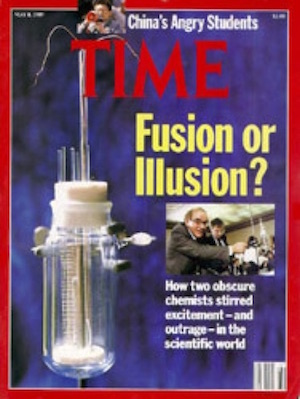
\includegraphics[width=0.5\linewidth]{_images/FalseResults} 

}

\caption{Consequences of a wrong experiment, producing bad data.}\label{fig:figName2}
\end{figure}

Apart from that famous example, we need to go back to our original question: how can we be sure that the data are accurate? The answer is simple: we can never be totally sure, but \textbf{we should strive to apply research methods as rigorous as possible, so that we can be as sure as possible that the experiment is `valid'}, i.e.~that it does not contain any sources of systematic error (bias). In other words, good data come as the consequence of valid methods, which implies that \textbf{a scientific proof is such not because we are certain that it corresponds to the truth, but because we are reasonably certain that it was obtained by using valid methods}!

\hypertarget{the-falsification-principle}{%
\section{The `falsification' principle}\label{the-falsification-principle}}

The above approach has an important consequence: even if we have used a perfectly valid method and we have, therefore, produced a perfectly valid scientific proof, we can never be sure that we are right, because there could always be a future observation that says we are wrong. This is the basis of the `falsification theory,' as defined by Karl Popper (1902 -- 1994): we cannot demonstrate that our data are true, but we can only demonstrate that they are false.

In practice, going back to the scientific process, we start from our hypothesis, we design a valid experiment and obtain valid data. In case this data does not appear to contradict the hypothesis, we conclude that such a hypothesis is true because it has not been falsified. The hypothesis is held as true until new valid data arise that falsify it: in this instance, the hypothesis is rejected and a new one is defined and submitted to the falsification process.

The falsification theory has been very influential in science. I would like to highlight a few key-points.

\begin{enumerate}
\def\labelenumi{\arabic{enumi}.}
\tightlist
\item
  Science has nothing to do with truth or certainty. Science has a lot to do with uncertainty and we can never prove that a hypothesis is totally right. Therefore, we always organise experiments to reject hypothesis (i.e.~to prove that they are false)!
\item
  We need to use valid methods to ensure that random errors have been minimised, while systematic errors have been avoided as much as possible.
\item
  The remaining uncertainty due to residual random errors need to be quantified by using the appropriate stats and displayed along with the results.
\item
  Considering the residual uncertainty, we need to evaluate whether our data are good enough to falsify the original hypothesis. Otherwise, the experiment is inconclusive (but not necessarily the original hypothesis is true!)
\item
  If we have two competing hypothesis and they are equally good, we select the simplest one (Occam's razor principle)
\end{enumerate}

\hypertarget{trying-to-falsify-a-result}{%
\section{Trying to falsify a result}\label{trying-to-falsify-a-result}}

One aspect to be highlighted is that if I want to try and falsify a hypothesis which has been validated by a previous experiment, I need to organise a confirmatory experiment. In this frame, we need to distinguish between:

\begin{enumerate}
\def\labelenumi{\arabic{enumi}.}
\tightlist
\item
  replicability
\item
  reproducibility
\end{enumerate}

An experiment is replicable when it gives the same results when repeated in the very same conditions. This explains why an accurate descriptions of materials and methods is fundamental to every scientific report: how could we repeat an experiment without knowing all detail about it?

Unfortunately, field experiments in agriculture are very seldom replicable, due to the environmental conditions, which change unpredictably from one season to the other. Therefore, we can only try to demonstrate that an experiment is reproducible, that is to say that it gives similar results when it is repeated in different conditions. Of course, failing to reproduce the results of an experiment in different conditions does not necessarily negate the validity of the original results.

This latter aspect is relevant. Think about Newton's gravitation law, which has always worked very well to predict the motion of planets as well as objects on Earth. This law was falsified by Einstein's studies, but it was not totally abandoned; indeed, within the limits of the conditions where it was proved, Newton's laws are still valid and they are good enough to be used for relevant tasks, such as to plan the trajectory of rockets.

\begin{center}\rule{0.5\linewidth}{0.5pt}\end{center}

\hypertarget{the-basic-principles-of-experimental-design}{%
\section{The basic principles of experimental design}\label{the-basic-principles-of-experimental-design}}

So far, we have seen that we need good data to express scientific claims and, to have good data, we need a valid experiment. A good methodology for designing experiments has been described by the English scientist Ronald A. Fisher (1890 - 1962). He graduated in 1912 and worked for six years as a statistician for the City of London, until he became a member of the Eugenics Education Society of Cambridge, founded in 1909 by Francis Galton, the cousin of Charles Darwin. After the end of the First World War, in 1919 he was offered a position at the Galton Laboratory at the University College of London, led by Karl Pearson, but he refused, due to profound rivalry with Pearson himself. Therefore, he begun working at the Rothamsted Experimental Station (Harpenden), where he was busy analysing the vast body of data that had accumulated starting from 1842. During this period, he invented the analysis of variance and defined the basis for valid experiments, publishing his results in the famous book ``The design of experiments,'' dating back to 1935.

In summary, Fisher recognised that a valid experiment must adhere to three fundamental principles:

\begin{enumerate}
\def\labelenumi{\arabic{enumi}.}
\tightlist
\item
  control;
\item
  replication;
\item
  randomisation.
\end{enumerate}

\hypertarget{control}{%
\subsection{Control}\label{control}}

The term `control' is very often mentioned in Fisher's book, with a number of different meanings. Perhaps, the most convincing definition is given at the beginning of Chapter 6: \emph{`control' consists of establishing controlled conditions, in which all factors except one can be held constant}. We can slightly widen this definition by saying that there should not be any difference between experimental units, apart from those factors which are under investigation.

The above definition sets the basis for what we call a \emph{comparative experiment}; I will better explain this concept by using an example. Just assume that we have found a revolutionary fertiliser and we want to compare it with a traditional one: clearly, we cannot use the innovative fertiliser in one field and compare the observed yield with that obtained in the previous season with the traditional fertiliser. We all understand that, apart from the fertiliser, several environmental variables changed from one season to the other.

A good controlled experiment would consist of using two field plots next to each other, with the same environmental condition, soil, crop genotype and everything else, apart from the fertiliser, which will be different for the two plots. In these conditions, the observed yield difference shall be reasonably attributed to the fertiliser.

Apart from isolating the effect under study, a good control is exerted by using the greatest care to minimise the effects of all potential sources of experimental error. This may seem obvious, but putting it into practice may be overwhelming. Indeed, different types of experiments will require different types of techniques and the best to do to master those techniques is `learning by doing,' preferably under the supervision of an expert technician. I will only underline three general aspects:

\begin{enumerate}
\def\labelenumi{\arabic{enumi}.}
\tightlist
\item
  methodological rigour
\item
  accurate selection of experimental units
\item
  avoiding intrusions
\end{enumerate}

Methodological rigor refers to the soundness or precision of a study in terms of planning, data collection, analysis, and reporting. It is obvious that, if we intend to study the degradation of a herbicide at 20°C we need an oven that is able to keep that temperature constant, the herbicide needs to be thoroughly mixed with the soil at the exact concentration and we need to use a well calibrated instrument as well as a correct protocol of analysis. However, we should never forget that there is a trade-off between methodological rigour/precision and the need for time and money resources, which is not independent from the aims of the experiment and the expected effect size. It is not necessary to attain a precision of 1 mL if we are determining the irrigation volume for maize!

In relation to the selection of experimental units, good control practices would suggest that we select very homogeneous individuals; by doing so, error is minimised and precision is maximised. However, we need to be careful: subjects also need to reliably represent the population from where they were selected. For instance, if we want to assess the effect of a particular diet, we could select cows of the same age, same weight and same sex, so that the diet effect is isolated from all other possible confounding effects. If we do so, we will probably obtain a very high precision, but our results will not allow for any sound generalisations to caws of other ages, weights and sex. Again, there is a trade-off between the homogeneity of experimental subjects and the possibility of generalisation.

Last, but not least, I would like to spend a few words about `intrusions,' i.e.~all the external events that occur and negatively impact on the experiment (e.g., drought, fungi attacks, aphids). Sometimes, these events are simply unpredictable and we will see that replication and randomisation (the other two principles of experimental design) are mainly meant to avoid that such intrusions produce systematic errors in our results. Some other times, these events are not totally unpredictable and they are named `demonic intrusions' by Hurlbert (1984) in a very influential paper (as opposed to the unpredictable non-demonic intrusions). The aforementioned author reports an example relating to a study about fox predation. If fences are used to avoid the entrance of foxes, but hawks use those fences as perches from which to search for a pray, in the end, foxes may be held responsible for the predation exerted by hawks. Therefore, we end up confounding the effect of an intrusion with the effect under investigation. Hurlbert concludes ``\emph{Whether such non-malevolent entities are regarded as demons or whether one simply attributes the problem to the experimenter's lack of foresight and the inadequacy of procedural controls is a subjective matter. It will depend on whether we believe that a reasonably thoughtful experimenter should have been able to foresee the intrusion and taken steps to forestall it}.''

\hypertarget{replication}{%
\subsection{Replication}\label{replication}}

In the previous paragraph, we have set the basis of a comparative experiment, wherein two plots put totally in the same conditions are treated with two different fertilisers. Of course, this is not enough to guarantee that the experiment is valid. Indeed, \emph{no one would now dream of testing the response to a treatment by comparing two plots, one treated and the other one untreated} (Fisher and Wishart, 1930; cited in Hurlbert, 1984).

In every valid experiment, the measurements should be replicated in more than one experimental unit, while non-replicated experiments are usually invalid. We can list four main reasons for replication:

\begin{enumerate}
\def\labelenumi{\arabic{enumi}.}
\tightlist
\item
  demonstrate that the measure is replicable (that does not mean it is reproducible, though);
\item
  ensure that any possible intrusions that affected one single experimental unit has not caused any relevant bias. Of course, the situation becomes troublesome if such an intrusion has affected all replicates! However, we will show that we can take care of this by using randomisation;
\item
  assess the precision of the experiment, by measuring the variability among replicates;
\item
  increase the precision of the experiment: the higher the number of replicates the higher the precision and the lower the uncertainty.
\end{enumerate}

The key issue about replication is that, to be valid, replicates must be truly independent, i.e.~the whole manipulation process to allocate the treatment must have been independently applied to the different replicates. This must be clearly distinguished from pseudo-replication, where at least part of the manipulation has been contemporarily applied to all replicates (Figure \ref{fig:figName2b}).

\begin{figure}

{\centering 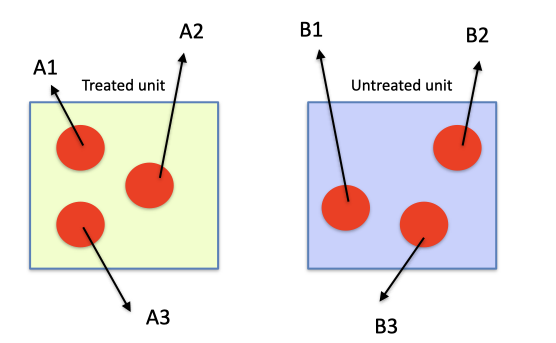
\includegraphics[width=0.75\linewidth]{_images/PseudoReplication} 

}

\caption{Schematic example of and invalid experiment, where pseudo-replication is committed}\label{fig:figName2b}
\end{figure}

Some typical examples of pseudo-replication are: (1) spraying a pot with five plants and measuring separately the weight of each plant, (2) treating one soil sample with one herbicide and making four measurements of concentration on four subsamples of the same soil, (3) collecting one soil sample from a field plot and repeating four times the same chemical analysis. In all the above cases, the treatments are applied only to one unit (pot or soil sample) and there are no true replicates, no matter how often the unit is sub-sampled. Clearly, if a random error is committed during the manipulation process, it carries over to all replicates and becomes a very dangerous systematic error.

In some cases, pseudo-replication is less evident and less dangerous; for example, when we have to spray a number of replicates with the same herbicide solution, we should prepare different lots of the same solution and independently spray them onto the replicated plots. In practise, very often we only prepare one solution and spray it onto all the replicates, one after the other. Strictly speaking, this would not be correct, because the manipulation is not totally independent: if we made a mistake while preparing the solution (e.g.~a wrong concentration), this would affect all replicates and would become a source of bias. However, such a practice is usually regarded as acceptable: if we sprayed the replicates independently, the amount of solution would too small to be precisely delivered by, e.g., a knapsack sprayer. As always, experience and common sense can be good guides to designing valid experiments.

Apart from some specific circumstances, the general rule is that valid experiments require true-replicates and pseudo-replication should never be mistaken for true replication, even in the case of laboratory experiments (Morrison \& Morris, 2000). You will learn by experience the exceptions to this rule, but we prefer to sound rather prescriptive in this respect: it is not nice to have a paper rejected because we did not menage to convince the editor that our lack of true-replication should be regarded as justified!

One common question is: how many replicates do we need? In this respect, we need to find a good balance between precision and costs: four replicates are usually employed in field experiments, although also three is a common value, when the effects are expected to be rather big and we have a small budget. A higher number of replicates is not very common, mainly because the size of the experiment becomes rather big and, consequently, soil variability increases as well.

\hypertarget{randomisation}{%
\subsection{Randomisation}\label{randomisation}}

Control and true-replication, in themselves, do not guarantee that the experiment is valid. Indeed, some innate characteristics of experimental units or some random intrusion might systematically influence all replicates of one treatment, so that the effect of such disturbance is confounded with the effect of the experimental treatment. For example, think that we have a field with eight plots, along a positive gradient of fertility, as shown in Figure \ref{fig:figName2c}; if we treat the plots from 1 to 4 with the fertiliser A and the plots from 5 to 8 with the fertiliser B, a possible difference between the means for A and B might be wrongly attributed to the treatment effect, while it might be due to the innate difference in fertility (confounding effect).

\begin{figure}

{\centering 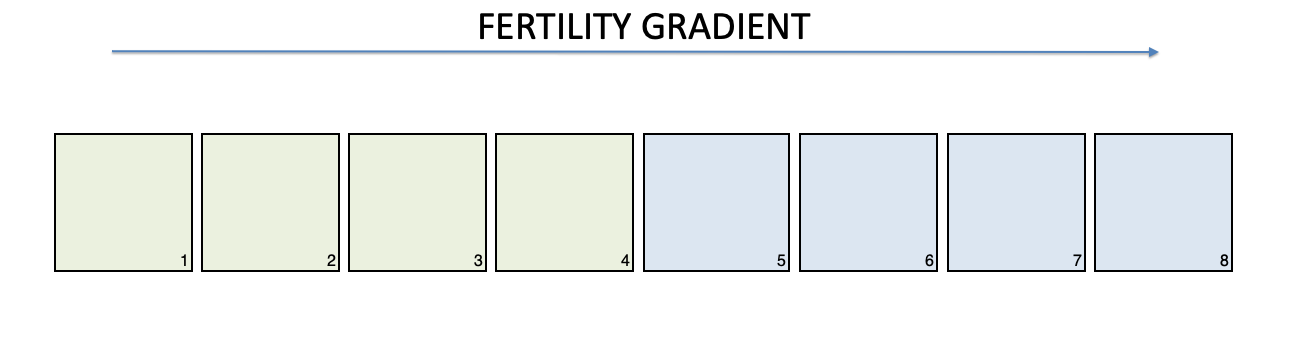
\includegraphics[width=1.05\linewidth]{_images/LackRandomisation} 

}

\caption{Example of lack of randomisation: the colours identify two different experimental treatments}\label{fig:figName2c}
\end{figure}

Randomisation is usually performed by way of random allocation of treatments to the experimental units, which is typical of \textbf{manipulative experiments}. In the case of field experiments, randomisation can also relate to random spatial and temporal dispersion, as we will see in the next Chapter.

The allocation of treatments is not always possible, as it may sometimes be impractical, unethical or illegal. For example, if we want to assess the efficacy of seat belts, designing an experiment where people are sent out either with or without fastened seat belts is neither ethical nor legal. In this case, we can only record, retrospectively, the outcome of previous accidents.

In this type of experiment we do not allocate the treatments, but we observe units that are `naturally' treated (\textbf{observational experiment}); therefore, randomisation is obtained by random selection of individuals.

As the result of using proper randomisation, all experimental units are equally likely to receive any type of disturbance/intrusion, so that the probability that all replicates of the same treatment are affected is minimal. Therefore, confounding the effect of a treatment with other types of systematic effects, if not impossible, is made highly unlikely.

\hypertarget{invalid-experiments}{%
\section{Invalid experiments}\label{invalid-experiments}}

Let's go back to the beginning of this chapter: how do we recognise real science from pseudo-science? By now, we should have learnt that reliable scientific information comes from data obtained in valid experiments. And we should have also learnt that experiments are valid if (and only if) they are properly controlled, replicated and randomised: the lack of any of these fundamental traits makes the results more or less unreliable and doubtful.

In our experience as reviewers and statistical consultants, we have found several instances of invalid experiments. It is a pity: in such cases, the paper is rejected and there is hardly any remedy to a poorly designed experiment. The most frequent problems are:

\begin{enumerate}
\def\labelenumi{\arabic{enumi}.}
\tightlist
\item
  lack of good control
\item
  `Confounding' and spurious correlation
\item
  Lack of true replicates and/or careless randomisation
\end{enumerate}

The consequences may be very different.

\hypertarget{lack-of-good-control}{%
\subsection{Lack of good control}\label{lack-of-good-control}}

In some cases, experiments are not perfectly controlled. Perhaps, this statement is difficult to be interpreted, as no experiments can, indeed, be perfectly controlled: even if we have managed to totally avoid measurement errors, subject-to-subject variability and sampling variability can never be erased. Therefore, in terms of control, how do we draw the line between a valid and an invalid experiment? The suggestion is to carefully check whether the control was good enough not to impact on accuracy. If the experiment was only imprecise, the results do not loose their validity, although they may not be strong enough to reject our initial hypothesis. In other words, imprecise experiments are valid, but, very often, inconclusive. We say that they are not powerful.

An experiment becomes invalid when there are reasons to suspect that the lack of good control impacted on data accuracy (wrong sampling, systematic errors, invalid or unacceptable methods). In this case, the experiment should be rejected, because it might be reporting measures that do not correspond to reality.

\hypertarget{confounding-and-spurious-correlation}{%
\subsection{`Confounding' and spurious correlation}\label{confounding-and-spurious-correlation}}

Reporting wrong measures is dangerous but \textbf{confounding} is even worse. It happens when the effect of some experimental treatments is confounded with other random or non-random systematic effects. The risk is particularly high with observational experiments. For example, if we observe the relative risk of death for individuals who were naturally exposed to a certain risk factor compared to individuals who were not exposed, the experimental outcome can be affected by several uncontrollable traits, such as sex, height, weight, age and so on. Therefore, we have a stimulus (exposure factor), a response (risk of death) and other external variables, which we call the `confounders.' If one of the confounders is correlated both with the response and with the stimulus, a `spurious' correlation may appear between the stimulus and the response, which does not reflect any real causal effects (Figure \ref{fig:figName2d}).

\begin{figure}

{\centering 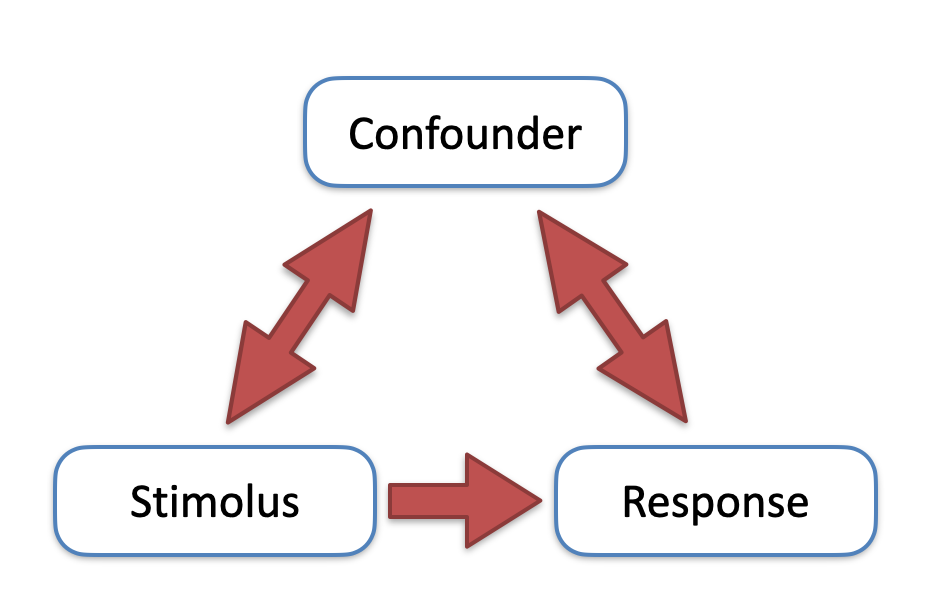
\includegraphics[width=0.75\linewidth]{_images/Confounding} 

}

\caption{Graphical representation of spurious correlation: an external confounder influences both the stimulus and the response, so that these two latter variables are correlated}\label{fig:figName2d}
\end{figure}

One typical example of spurious correlation has been found between the number of churches and the number of crimes in American cities. Such a correlation, in itself, does not prove that one factor (religiosity) causes the other one (crime); a thorough explanation should consider the existence of a possible confounder, such as the density of population: big cities have more inhabitants and, consequently, more churches and more crimes with respect to small cities. Accordingly, religiosity and crime are related to density and are related to each other, but such a relationship os only spurious.

In the web, we can found a lot of other funny examples of spurious correlations, such as between the consumption of sour cream over years and the number of motorcycle riders killed in accidents (Figure \ref{fig:figName22}). In this case, the lack of any scientific bases is clear; in other cases, it may be more difficult to spot. A very witty saying is: ``correlation does not mean causation''; please, do not forget it!

\begin{figure}

{\centering 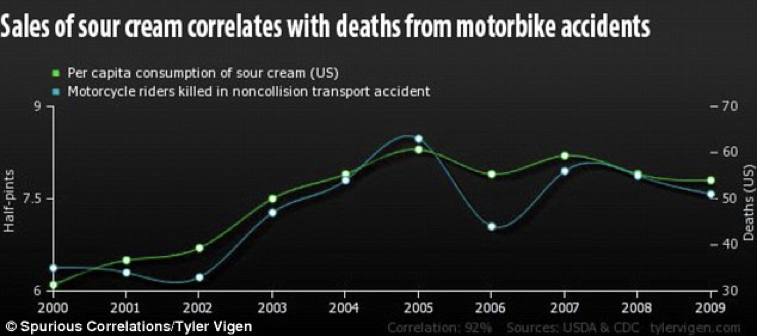
\includegraphics[width=0.9\linewidth]{_images/PannaAcida} 

}

\caption{Esempio di correlazione spuria}\label{fig:figName22}
\end{figure}

\hypertarget{lack-of-true-replicates-or-careless-randomisation}{%
\subsection{Lack of true-replicates or careless randomisation}\label{lack-of-true-replicates-or-careless-randomisation}}

Some issues that may lead to the immediate rejection of scientific papers are:

\begin{enumerate}
\def\labelenumi{\arabic{enumi}.}
\tightlist
\item
  there are pseudo-replicates, but no true-replicates
\item
  true-replicates and pseudo-replicates are mistaken
\item
  there is no randomisation
\item
  randomisation was constrained, but the constraint has not been accounted for in statistical analyses.
\end{enumerate}

It is very useful to take a look at the classification made by Hurlbert (1984), which we present in Figure \ref{fig:figName23}.

\begin{figure}

{\centering 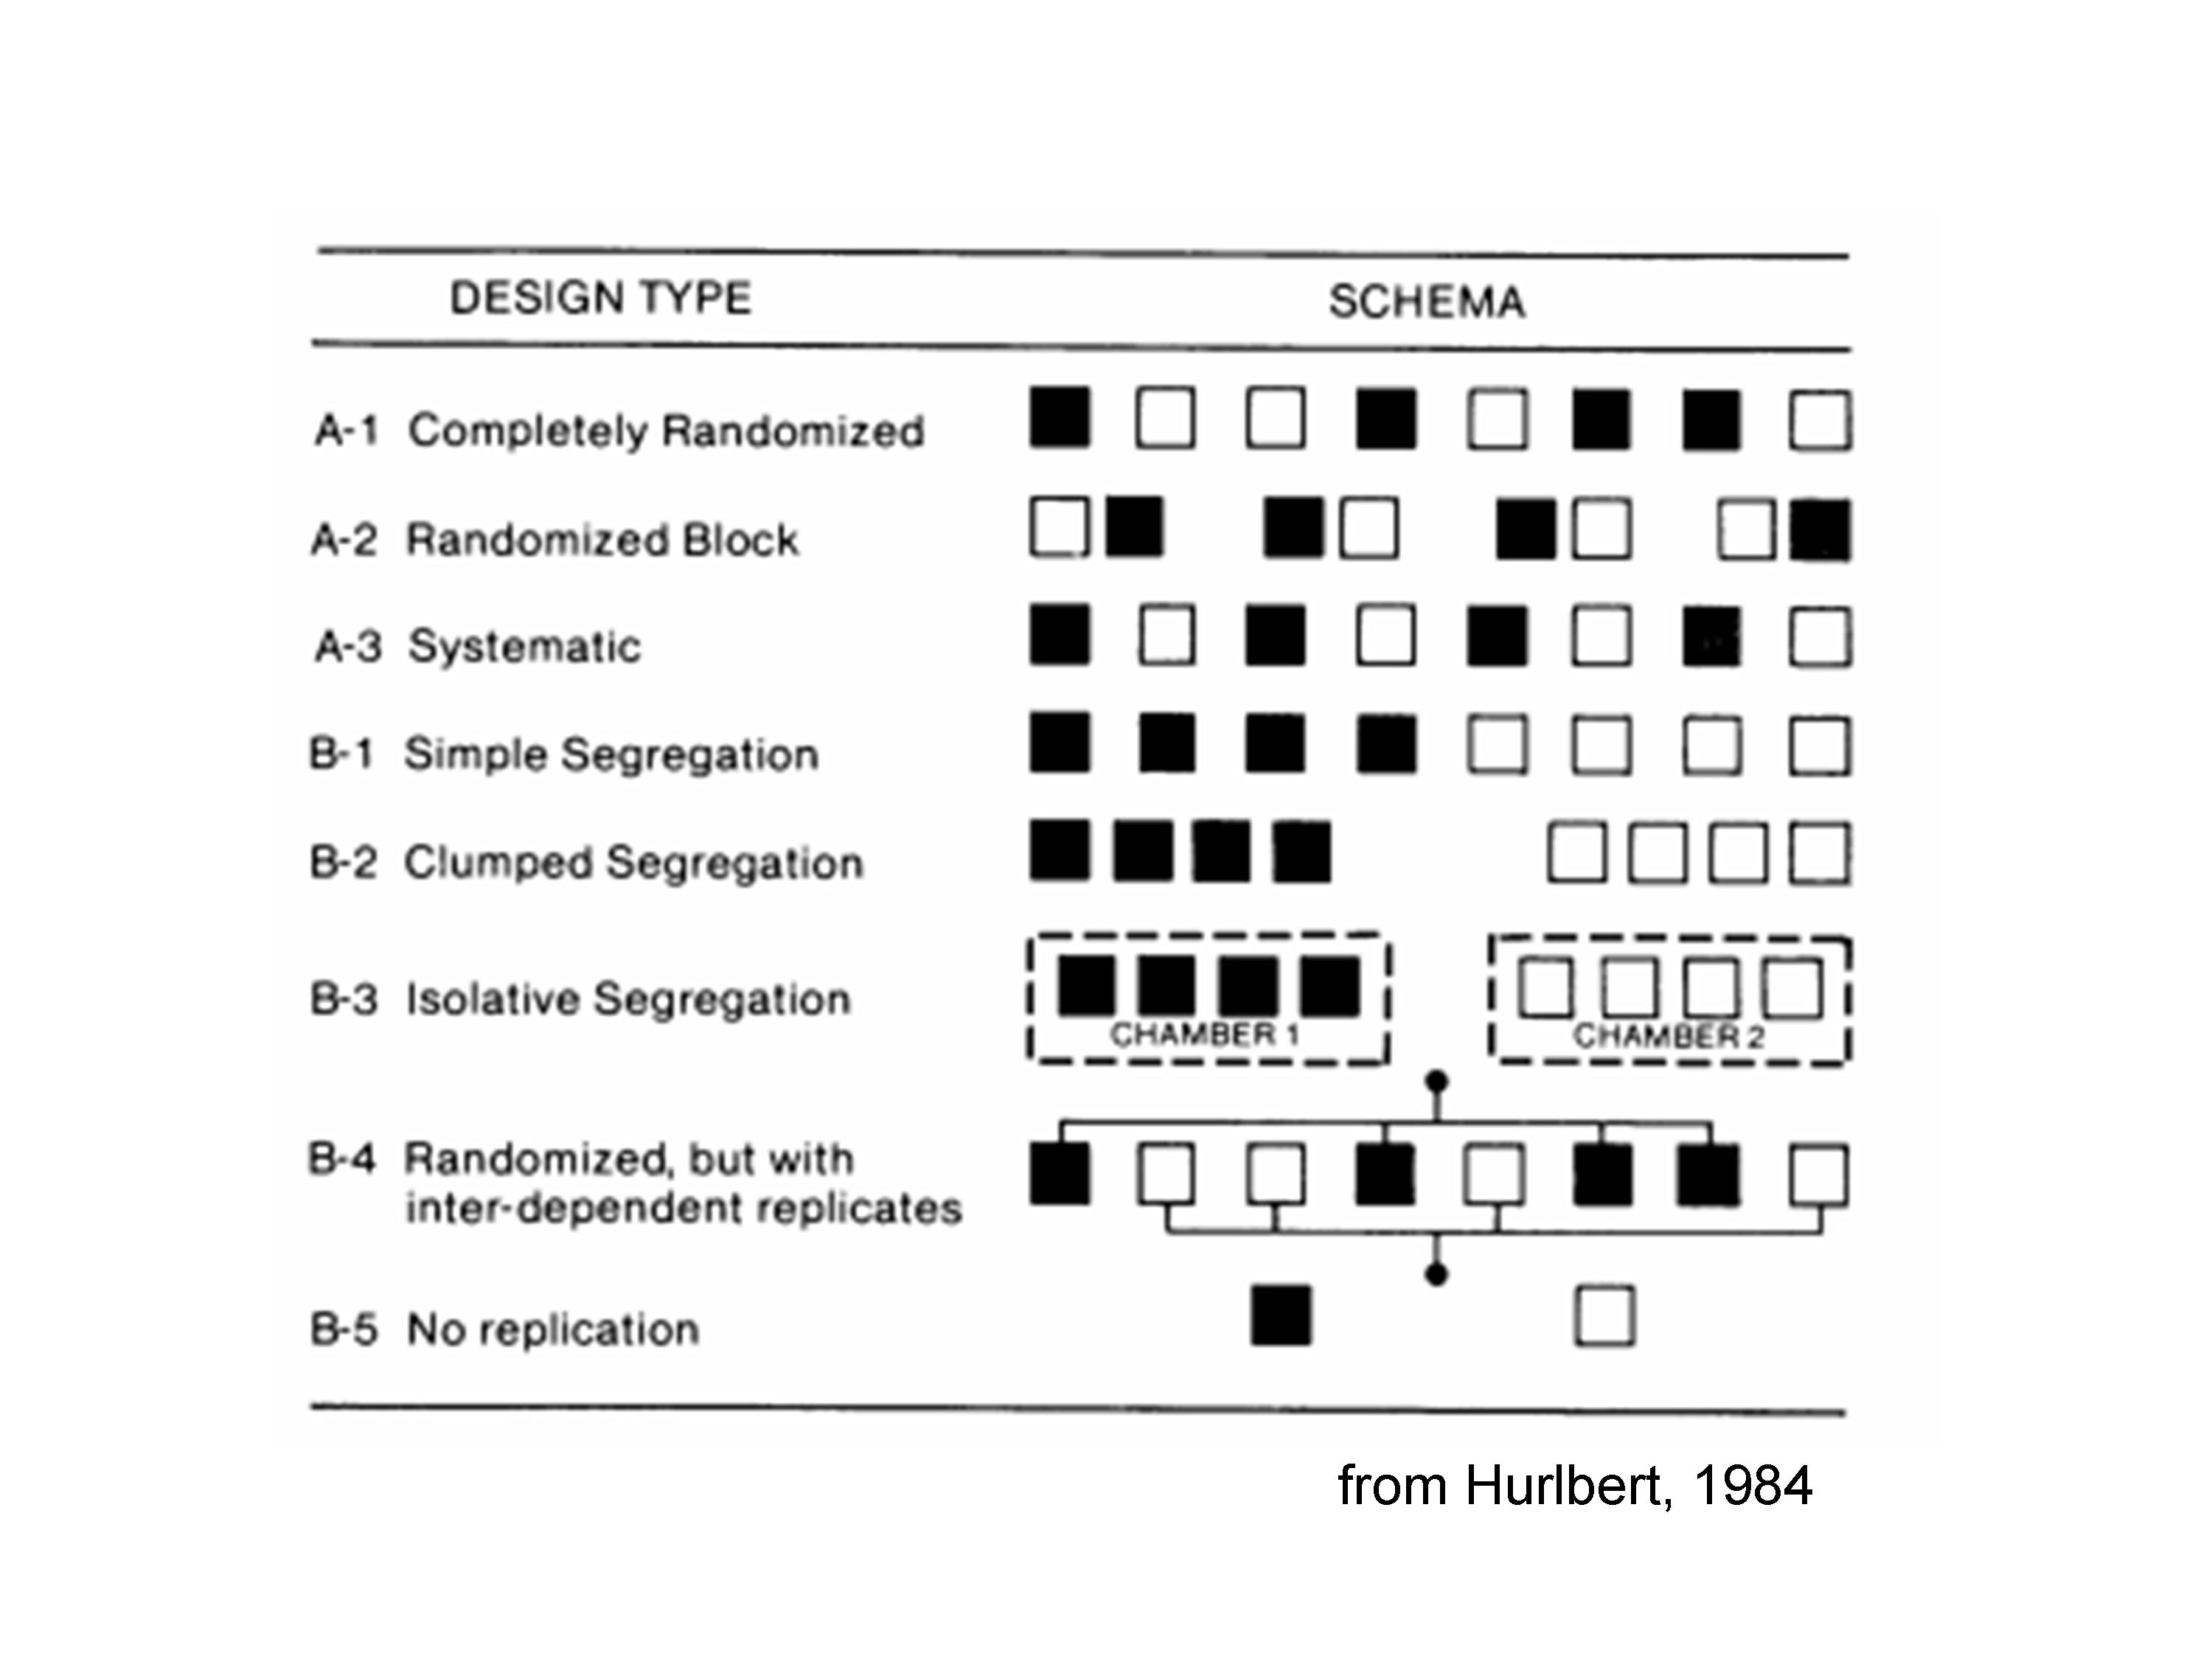
\includegraphics[width=0.9\linewidth]{_images/Randomisation} 

}

\caption{Different types of randomisations, although they are not all correct (taken from: Hurlbert, 1984)! See the text for more explanations.}\label{fig:figName23}
\end{figure}

It shows eight experimental subjects, to which two treatments (black and white) were allocated, by using eight different experimental designs. Design A1 is perfectly valid, as the four `white' units and the four `black' units were randomly selected.

Design A2 is correct, although the randomisation was not complete; indeed, we divided the units in four groups and, within each group, we made a random selection of the `white' and `black' individual. This is an example of constrained randomisation, as the random selection of individuals is forced to take place within each group. We will see that such a constraint is correct, but it must be taken into account during the process of data analysis.

Design A3 looks suspicious: there are true replicates, but treatments were not randomly, but systematically allocated to experimental units. Indeed, black units are always to the right of white units; what would happen in case of a latent right-to-left fertility gradient? Black units would be advantaged and the treatment effect and fertility effect would be confounded. Such suspect may lead to an invalid experiment. Systematic allocation of treatments may be permitted in some instances, when a spatial-temporal sequence has to be evaluated. For example:

\begin{enumerate}
\def\labelenumi{\arabic{enumi}.}
\tightlist
\item
  when we have four trees and we want to compare the yield of a low branch with the yield of a high branch. Clearly, low and high branches are systematically ordered and cannot be randomised;
\item
  when we need to compare herbicide treatments in two timings (e.g., pre-emergence and post-emergence); clearly, one timing is always before the other one;
\item
  when we need to compare the amount of herbicide residuals at two different depths, which are always ordered along the soil profile.
\end{enumerate}

In those conditions, the experiment is valid even when the randomisation follows a systematic pattern.

Design B1 is usually invalid: there is no randomisation and the systematic allocation of treatments creates the segregation of units, which are not interspersed. The treatment effect can be easily confounded with any possible location effects (right vs.~left). Also for design B1, there are a few exceptions were such a design could be regarded as valid, e.g., when we want to compare two locations, two regions, two fields, two lakes or any other physically parted conditions. Such location effects need to be evaluated with great care, as we are rarely in the condition of clearly attributing the effect to a specific agronomic factor. For example, two locations can give different yields because of different soil, different weather, different sowing times and so on.

Design B2 and B3 are analogous to B1, even though the location effects are usually bigger. Isolative segregation is typical of growth chamber experiments; for example, we can use such a design to compare the germination capability at two different temperatures, by using two different ovens. In this case the temperature effect is totally confounded with the oven effect; it may not be problem in case the two ovens are very similar, but it is clear that any malfunctioning of one of the two ovens will be confounded with the treatment effect. Furthermore, the different replicates in one oven are not, indeed, true replicates, because the temperature treatment is not independently allocated (pseudo-replicates).

Design B4 is a general example of pseudo-replication, where replicates are inter-dependent; we have already given other examples in the previous paragraphs. Designs lacking true-replicates are generally invalid, unless true-replicates are also included. For example, if we have four ovens that are randomly allocated to two temperatures (two ovens per temperature) and we have four Petri dishes per oven, there are two true-replicates and four pseudo-replicates per replicate. The design is valid, although we should keep true-replicates and pseudo-replicates clearly parted during data analysis, i.e.~we should not behave as if we had 4 \(\times\) 2 = 8 true-replicates!

Design B5 is clearly invalid, due to total lack of replication.

\hypertarget{how-can-we-assess-whether-the-data-is-valid}{%
\section{How can we assess whether the data is valid?}\label{how-can-we-assess-whether-the-data-is-valid}}

As we said, we have to check the methods. However, in everyday life this is very seldom possible. Indeed, we may not be expert enough to spot possible shortcomings and, above all, the methods may not detailed in newspapers and magazines, which limit themselves to reporting the result. What can we do, then? The answer is simple: we have to carefully check the sources.

Authoritative scientific journals publish manuscripts only after a process of `\emph{peer review}.' In practise, the submitted manuscript is managed by the handling editor, who reads the paper and sends it to one to three widely renowned experts (\emph{reviewers}). The editor and reviewers carefully inspect the paper and decide whether it can be published either as it is, or after revision, or, on the other hand, it should be rejected. After this process, we can be reasonably sure that the results are reliable and there are no important shortcomings that would make the experiment invalid. The peer review process is rather demanding for authors and it may require months and two-three reviews before the paper is accepted. We have found a nice picture at \href{http://scienceblogs.com/startswithabang/2013/06/07/the-4-jobs-of-a-referee-in-peer-review/}{scienceBlog.com}, which summarises rather well the feelings of a scientists during the reviewing process (Figure \ref{fig:figName3}).

\begin{figure}

{\centering 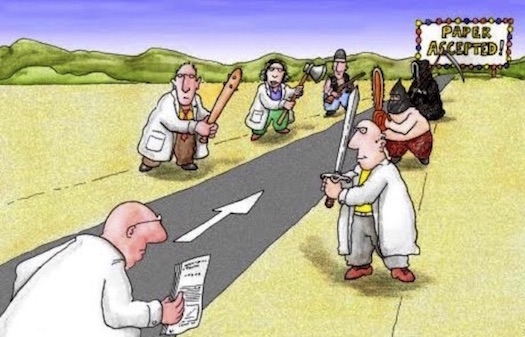
\includegraphics[width=0.75\linewidth]{_images/PeerReview} 

}

\caption{The peer review process}\label{fig:figName3}
\end{figure}

\hypertarget{conclusions}{%
\section{Conclusions}\label{conclusions}}

In the end, we can go back to our initial question: ``How can we draw the line between science and pseudoscience?'' The answer is that science is based on reliable data, obtained in valid scientific experiments, wherein every possibile source of systematic errors and confounding has been properly controlled and minimised. In particular, we have seen that every valid experiment should adhere to three fundamental principles, i.e.~control, replication and randomisation.

In practice, making sure that the methods were appropriate may require a specific expertise in a certain research field. Therefore, our `take-home message' is: unless we are particularly expert in a given subject, we should always make sure that the results were published in authoritative journals and selected by a thorough peer review process.

\begin{center}\rule{0.5\linewidth}{0.5pt}\end{center}

\hypertarget{further-readings}{%
\section{Further readings}\label{further-readings}}

\begin{enumerate}
\def\labelenumi{\arabic{enumi}.}
\tightlist
\item
  Fisher, Ronald A. (1971) {[}1935{]}. The Design of Experiments (9th ed.). Macmillan. ISBN 0-02-844690-9.
\item
  Hurlbert, S., 1984. Pseudoreplication and the design of ecological experiments. Ecological Monographs, 54, 187-211
\item
  Kuehl, R. O., 2000. Design of experiments: statistical principles of research design and analysis. Duxbury Press (CHAPTER 1)
\item
  Morrison, D.A. and Morris, E.C., 2000. Pseudoreplication in experimental designs for the manipulation of seed germination treatments. Austral Ecology 25, 292--296.
\item
  Wollaston V., 2014. Does sour cream cause bike accidents? No, but it looks like it does: Hilarious graphs reveal how statistics can create false connections. Published at: \url{https://www.dailymail.co.uk/sciencetech/article-2640550/Does-sour-cream-cause-bike-accidents-No-looks-like-does-Graphs-reveal-statistics-produce-false-connections.html}. Date of last access: 03/09/2020.
\end{enumerate}

\hypertarget{designing-experiments}{%
\chapter{Designing experiments}\label{designing-experiments}}

\hypertarget{the-elements-of-research}{%
\section{The elements of research}\label{the-elements-of-research}}

In the previous chapter we have seen that every valid experiment should adhere to three fundamental principles, i.e.~control, replication and randomisation. You may wonder: how do we put such principles into practice? Of course, there is not an easy and general answer: setting up a good experiment is mainly a matter of experience and the tuition of an experienced colleague is essential, especially while moving the first steps in the research world.

In this chapter, we will focus on some common elements that we need to care about for all experiments, of any type. These elements are:

\begin{enumerate}
\def\labelenumi{\arabic{enumi}.}
\tightlist
\item
  the hypothesis and objectives;
\item
  the experimental treatments;
\item
  the experimental units;
\item
  the allocation of treatments to units;
\item
  the response variables.
\end{enumerate}

All detail about those elements need to be clearly given at the beginning of every good research project, report or scientific manuscript.

\hypertarget{hypothesis-and-objectives}{%
\section{Hypothesis and objectives}\label{hypothesis-and-objectives}}

The Galilean process of research starts from a well founded hypothesis, i.e.~a predictive statement about the possible outcome of a certain biological system. Such an hypothesis is usually based on an accurate review of literature information and, possibly, on a set of preliminary experiments. It must be:

\begin{enumerate}
\def\labelenumi{\arabic{enumi}.}
\tightlist
\item
  relevant;
\item
  clearly defined;
\item
  specific;
\item
  testable.
\end{enumerate}

A well set hypothesis leads naturally to the definition of the objectives of the experiment, which must be:

\begin{enumerate}
\def\labelenumi{\arabic{enumi}.}
\tightlist
\item
  realistic;
\item
  achievable;
\item
  measurable;
\item
  time constrained.
\end{enumerate}

Objectives should always be phrased in such a way that it is possible to exactly identify the moment when they have been achieved. For complex research projects, involving more than one experiment, it may be useful to define a general objective and several specific objectives, organised in successive phases, so that it is easy to check the progress of the research study and to revise the time schedule, in case some unexpected problems arise.

Unclear objectives may lead to inefficient research, wherein unnecessary data are collected, while relevant observations are left out.

\hypertarget{the-experimental-treatments}{%
\section{The experimental treatments}\label{the-experimental-treatments}}

Once the objectives are clear, we need to define the experimental `stimuli' that will be allocated to the experimental units. A set of related `stimuli' is called the \textbf{experimental factor}; for example, if we want to compare the genotypes A, B and C, we have the genotype factor with three levels. If we have one factor with a unique level, we usually talk about \emph{mensurative experiment}, otherwise, we talk about \emph{comparative experiment}, which is, by far, the most common situation.

\hypertarget{factorial-experiments}{%
\subsection{Factorial experiments}\label{factorial-experiments}}

When we have two (or more) experimental factors, we could either make separate experiments, or we could make a \textbf{factorial experiment}, wherein we combine the levels of the two factors. This second solution is much more interesting, because we can assess possible interaction effects between the two factors (we will talk about this in Chapter 12).

Factorial experiments may be planned in two different ways, i.e.~they can be \textbf{crossed} or \textbf{nested}. In a crossed design, we have all possible combinations between the levels for all factors; for example, if we want to compare three sunflower genotypes (A, B and C) at two different nitrogen rates (N1 and N2), a crossed factorial experiment should include all the six combinations A-N1, A-N2, B-N1, B-N2, C-N1 and B-N2. Otherwise, in a nested design, the levels of one factor are different, depending on the level of the other factor; for example, if we want to compare organic farming and conventional farming by using the most suitable maize genotypes for each agricultural system, we should use a nested design.

Recognising crossed and nested factorial designs is important, because the resulting data needs to be analysed in different ways.

\hypertarget{the-control}{%
\subsection{The control}\label{the-control}}

Very often, comparative experiments need a suitable \emph{control} or \emph{check} level, which is used as the reference against which all other treatments are evaluated. We can include either:

\begin{enumerate}
\def\labelenumi{\arabic{enumi}.}
\tightlist
\item
  an untreated control,
\item
  a control treated with a placebo, or
\item
  a control treated with ordinary practices.
\end{enumerate}

For example, in a genotype experiment we usually include a reference genotype that is very widely grown in all nearby farms. For herbicide experiments, we always include an untreated control, which is fundamental to assess the composition of weed flora and quantify weed control efficacy for all herbicides under investigation. Furthermore, we can also include a weed-free control (usually hand-weeded) as the reference to evaluate possible symptoms of herbicide phytotoxicity to the crop. In toxicology, the untreated control may be replaced by a control treated with a placebo, i.e.~a compound containing the same components of the experimental treatment, except the active ingredient. The placebo is usually necessary when:

\begin{enumerate}
\def\labelenumi{\arabic{enumi}.}
\tightlist
\item
  the experimental subject (usually a human) perceives its condition and reacts to the expectation about the efficacy of the chemical under investigation;
\item
  the commercial formulation, apart from the active ingredient, contains other components, such as adjuvants, surfactants and other substances which may show some sort of biological effects.
\end{enumerate}

\hypertarget{the-experimental-units}{%
\section{The experimental units}\label{the-experimental-units}}

The experimental unit is the physical entity to which the treatment is allocated, e.g.~a plant, a plot, an animal, a pot. In this respect, we need to be careful to clearly distinguish the experimental units from the observational units; indeed, we can allocate the treatment to a field plot and measure several plants therein or we can allocate the treatment to a tree and measure several leaves on that tree. A clear distinction between experimental units and observational units can help us avoid problems with pseudo-replication (see Chapter 1).

The experimental units are always selected from a wider population of interest. For example, we select the plots from a field, the plants from a crop or some animals from a herd. A sample should be representative and homogeneous, although these may be two contrasting characteristics. Indeed, if we select very homogeneous individuals, we run the risk of getting a sample that no longer represents the whole population, but only a subset of it. For example, if our sample was composed by adult male bovines in good health, it may not necessarily represent a population composed also by females, young and diseased animals. Sampling a population of interest in a proper way may be a daunting task, especially in the social sciences. Several sampling protocols have been defined (e.g., random sampling, systematic sampling, stratified sampling, clustered sampling, convenience sampling, quota sampling, \ldots), which are far beyond the scope of this book; you can read Daniel (2011) for a thorough explanation.

In some cases, the process of sampling is less obvious, but that does not mean that there is no sampling. For example, in manipulative laboratory experiments, the experimental units are specifically prepared for each assay, such as the pots for a herbicide assay or the Petri dishes for a germination assay. Even if there is no real selection process, these units should be regarded as sampled from the wider population of pots or Petri dishes that we could have possibly prepared.

\hypertarget{the-allocation-of-treatments}{%
\section{The allocation of treatments}\label{the-allocation-of-treatments}}

Unless we select experimental units that are `naturally treated' (observational experiments; see Chapter 1), one central issue of every experiment is the technique we use to allocate the treatments. In general, following Fisher's principles, we should pursue a completely randomised allocation, although, in some circumstances, it may be advantageous to put some constraints, as long as such constraints are not neglected during the process of data analysis. Constraints are very common in field experiments and we will see that they set the basis for the so-called \textbf{experimental layout}.

In some cases, it is appropriate to hide some detail of the allocation process; for example, in medical research, it may be necessary that the subjects are not aware about which treatment they are going to receive (\textbf{single-blind experiments}), in order to avoid possible unconscious effects. In agriculture, it is often necessary that the researcher is not aware about which treatment was allocated to each unit, in order to avoid that the objectivity of visual and sensory assessments is undermined. If neither the subjects nor the researcher are aware about the treatment, we talk about \textbf{double-blind experiments}.

\hypertarget{the-variables}{%
\section{The variables}\label{the-variables}}

At the end of an experiment we produce a set of data (dataset), which is composed by a collection of variables. These variables describe the experimental units in relation to some of their characteristics and we usually distinguish (i) response variables, (ii) factor variables and (iii) accessory variables.

The response variables, obviously, describe the response of units to the experimental treatments (e.g., the yield, the weight, the height, and so on), while the factor variables describe the experimental stimulus allocated to each unit (e.g., the tillage method, fertilisation rate, genotype and so on). In some cases, we also record other accessory variables (or covariates), which measure potential confounding effects. For example, if we intend to study the yield of a number of trees, depending on how they are fertilised, the effect of tree age can act as a confounder. Therefore, if we cannot use trees of the same age, we can record the age as an accessory variable and use it to obtain a more reliable assessment of the fertilisation effect.

It is useful to classify the variables depending on their characteristics, into

\begin{enumerate}
\def\labelenumi{\arabic{enumi}.}
\tightlist
\item
  nominal variables;
\item
  ordinal variables;
\item
  count/ratio variables;
\item
  continuous variables.
\end{enumerate}

\hypertarget{nominal-variables}{%
\subsection{Nominal variables}\label{nominal-variables}}

Nominal variables are produced by assigning the subjects to a set of categories, such as dead/alive, germinated/ungerminated, red/blue/green, and so on. The categories can be two (\textbf{binomial response}) or more (\textbf{multinomial response}), they should not have any intrinsic ordering and should be mutually exclusive, in the sense that one individual can only belong to one category. With these variables, we can only count the number of individuals in each category (frequency), while other descriptive stats such as the mean and standard deviation are not used, at least not in the usual sense.

\hypertarget{ordinal-variables}{%
\subsection{Ordinal variables}\label{ordinal-variables}}

Ordinal variables are similar to nominal variables, but the categories are intrinsically ordered. For example, we could ask a farmer to express his appreciation for a certain agronomic practice, by using five categories, VERY LOW, LOW, AVERAGE, HIGH and VERY HIGH. The categories are mutually exclusive and ordered by increasing appreciation; thanks to such an ordering, we can calculate both the frequency in each category and the cumulative frequency, which is obtained by summing the frequency in each category to the frequencies in all the preceding categories (see next Chapter). With ordinal variables, descriptive statistics such as the mean can, sometimes, be calculated, as long as the distance between the categories is clearly defined.

\hypertarget{count-and-ratio-variables}{%
\subsection{Count and ratio variables}\label{count-and-ratio-variables}}

Sometimes the experimental units are characterised by some countable property; therefore, we can obtain a count for each unit and, consequently, a count variable. Please, note that this is different from a nominal/ordinal variable, where we count the units, not a specific trait in each single unit. For example, we obtain a count variable when we count the number of weeds in a plot, or the number of germinated seeds in a Petri dish, or the number of fruits per plant. When those counts have a predefined plateau, we can express them as relative to the plateau and obtain a ratio variable. For example, if we have ten seeds in a Petri dish, the count of germinated seeds may not exceed ten and it can be expressed as the proportion of germinated seeds. Both count and ratio data are discrete, in the sense that they can only take certain values (they are not continuous), but the mean and other descriptive stats can be be easily calculated with the usual method (see next Chapter).

\hypertarget{continuous-variables}{%
\subsection{Continuous variables}\label{continuous-variables}}

Continuous variables can take any value within a certain interval, such as the weight, height, yield, time and so on. It could be argued that every measurement instrument is characterised by its own resolution, below which all measurements take the same value. Therefore we could say that all continuous variable are, in practice, discrete. However, we can neglect this detail, as long as the resolution is high enough for practical purposes.

Continuous variables give a lot of information, although, in some instances, we may be interested in transforming them into ordinal variables, by using a classification procedure: we subdivide the range in classes (e.g.~\textless{} 50, 50-100, 100-150, \textgreater{} 150) and count the number of individuals in each class. This is often useful for descriptive purposes with big data, as we will see in the following chapter.

\hypertarget{sensory-and-visual-assessments}{%
\subsection{Sensory and visual assessments}\label{sensory-and-visual-assessments}}

In some instances, instead of measuring a certain trait of interest, we make visual or sensory assessments. For example, weed control ability and selectivity of herbicides can be assessed either by counting or weighing the survived weeds or by visual observations on a scale from 0 to 100\% (or similar scales). Sensory and visual assessments are rather common and give several advantages, such as:

\begin{enumerate}
\def\labelenumi{\arabic{enumi}.}
\tightlist
\item
  low cost,
\item
  high speed,
\item
  no need for costly instruments,
\item
  the possibility of disregarding the effect of external confounders. For example, when scoring the effect of an herbicide, an expert technician can easily distinguish phytotoxic effects from water stress damage and, thus, he can only consider the former effects, which would be impossible with objective weight measurements.
\end{enumerate}

Of course, there are also several disadvantages, such as:

\begin{enumerate}
\def\labelenumi{\arabic{enumi}.}
\tightlist
\item
  lower precision
\item
  subjectivity
\item
  we can be unconsciously influenced by knowing how the experimental unit has been treated
\item
  it may be difficult to keep a uniform judgment parameter throughout the survey
\item
  we need experience and training
\end{enumerate}

Sensory and visual data are largely acceptable in science, although their analysis may require some extra care and specific methods. Indeed, the resulting variable may resemble an ordinal variable (we assign one of a set of ordered categories), although the underlying scale is more or less continuous.

\hypertarget{setting-up-a-field-experiment}{%
\section{Setting up a field experiment}\label{setting-up-a-field-experiment}}

Once all the elements of an experiment have been carefully planned, we must be laid down such an experiment in practice. The techniques greatly vary depending on the disciplines, aims, scales (climatic chamber, greenhouse, laboratory, field and so on) and it is very difficult to provide general information, apart from reinforcing the idea that all valid experiments must controlled, replicated and randomised, as detailed in the previous chapter.

In this part, we will focus on the peculiar traits of field experiments, although most of the information relating to the experimental lay-out also applies to other types of experiments.

\hypertarget{selecting-the-field}{%
\subsection{Selecting the field}\label{selecting-the-field}}

Field selection is perhaps the key aspect for a successful experiment. First of all, a research field must be close enough to roads, laboratories and other facilities, which will permit a timely execution of sampling and measurements.

Secondly, we should not forget that there are countless reasons why a field experiment may turn out inconclusive, due to very wide environmental variability, relating to soil, weather, pests and so on. Therefore, at the onset of every experiment, we need to ensure that those sources of variability are kept to a minimum level, by selecting a very homogeneous field. We need to stay away from field parts with water stagnation, ditches, rows of trees and any other elements inducing an increase of variability in the behaviour of field crops.

Knowing the history of the field may also be rather important. Some previous crops (e.g., alfalfa or other legumes) may leave excess fertility in soil, which is not good if, e.g., a N-fertilisation experiment is to be set-up. Likewise, herbicide trials may leave non-homogeneous infestation levels, due to the presence of untreated controls and other low efficacy herbicides. The history of a field is also important, for herbicide and pest management experiments, as we may be interested in having/avoiding a certain weed or pest in our field.

If we suspect that there might be problems with soil heterogeneity, we should take some appropriate preliminary actions, such as growing a oat catch crop to remove excess soil nitrogen, growing alfalfa or other forage crops to suppress weed growth or perform deep ploughing to reduce the weed seed bank in the uppermost soil layer.

In order to enhance crop homogeneity, small plot experiments (see later) should be managed by suitable machinery, that is optimised to work on small surfaces; furthermore, some interventions (such as sowing, weeding and fertilising) can also be performed by hand. A peculiar technique that is often used to obtain a homogeneous crop density is sowing at overly high density and thin out to optimal density a few days after crop emergence.

\hypertarget{selecting-the-units-within-the-field}{%
\subsection{Selecting the units within the field}\label{selecting-the-units-within-the-field}}

Once we have selected a suitable field, we need to identify the experimental units. In this respect, we should distinguish:

\begin{enumerate}
\def\labelenumi{\arabic{enumi}.}
\tightlist
\item
  demonstrative on-farm trials
\item
  small plot research trials
\end{enumerate}

Demonstrative trials usually represent the final stage of research and they are usually conducted on commercial farms under realistic environmental and management conditions, considering all the inherent variability of farming systems. The aim is usually to obtain a reliable validation of new products, managements and technologies at the farm level; therefore, the experimental unit is usually the \textbf{strip}, i.e.~a long, rectangular piece of land, wherein the usual farming machinery (plough, planters, sprayers, combine harvester and so on) can be used.

The number of treatments under comparison is low and, most often, one new management practice (e.g.~crop management, crop protection, plant nutrition, and plant growth regulator) is compared to a local/farmer `control' in two contiguous strips. Such pair (the new management practice and the control) is a replicate; normally we should have a minimum of three (more is better) replicates for capturing within-field variability. For the sake of simplicity, considering the size of strips, randomisation may be omitted, so that the design resembles the type A-3 in Figure 1.4 (see previous chapter). One possible lay-out is shown in Figure \ref{fig:figName30a}, where we have four fields with two strips each; in one field, the first strip is assigned to one treatment and the second strip is assigned to the other.

\begin{figure}

{\centering 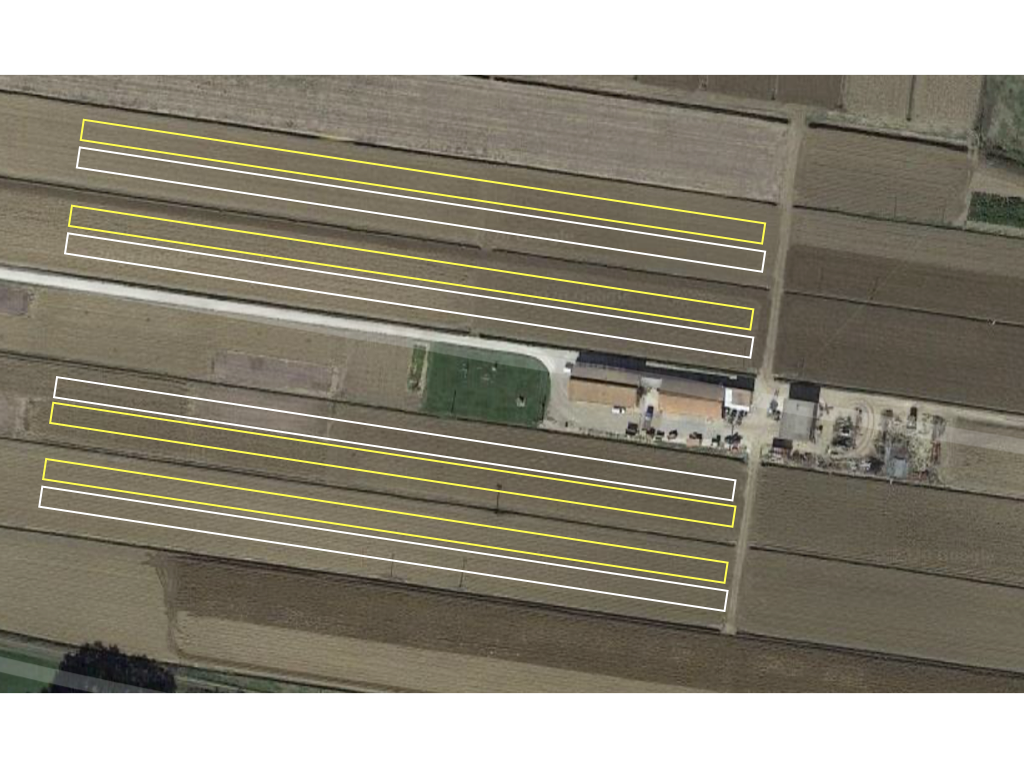
\includegraphics[width=0.9\linewidth]{_images/OnFarmTrial} 

}

\caption{The possible lay out of an on-farm trial, with four fields, two strips per field and a different treatment per strip (yellow and white)}\label{fig:figName30a}
\end{figure}

On-farm experiments are repeated across locations and growing seasons, so that we can have a better confidence in the selection of improved agronomic practices in new environments.

On the other hand, small plot experiments are in the middle between on-farm and laboratory experiments: they are set up in the field, but the experimental unit is represented by a \textbf{plot}, i.e.~a small piece of land, usually of 10 to 50 m\(^2\) surface (Figure \ref{fig:figName30b}). In small plot experiments we can keep a high degree of control for most confounding factors, while working in close-to-real conditions, which explains why this type of experiments is very widespread in the agricultural sciences. Of course, the observed yields in small plot experiments are usually 10-30\% higher than the corresponding yields in on-farm conditions, due to more careful management of all cropping practices.

\begin{figure}

{\centering 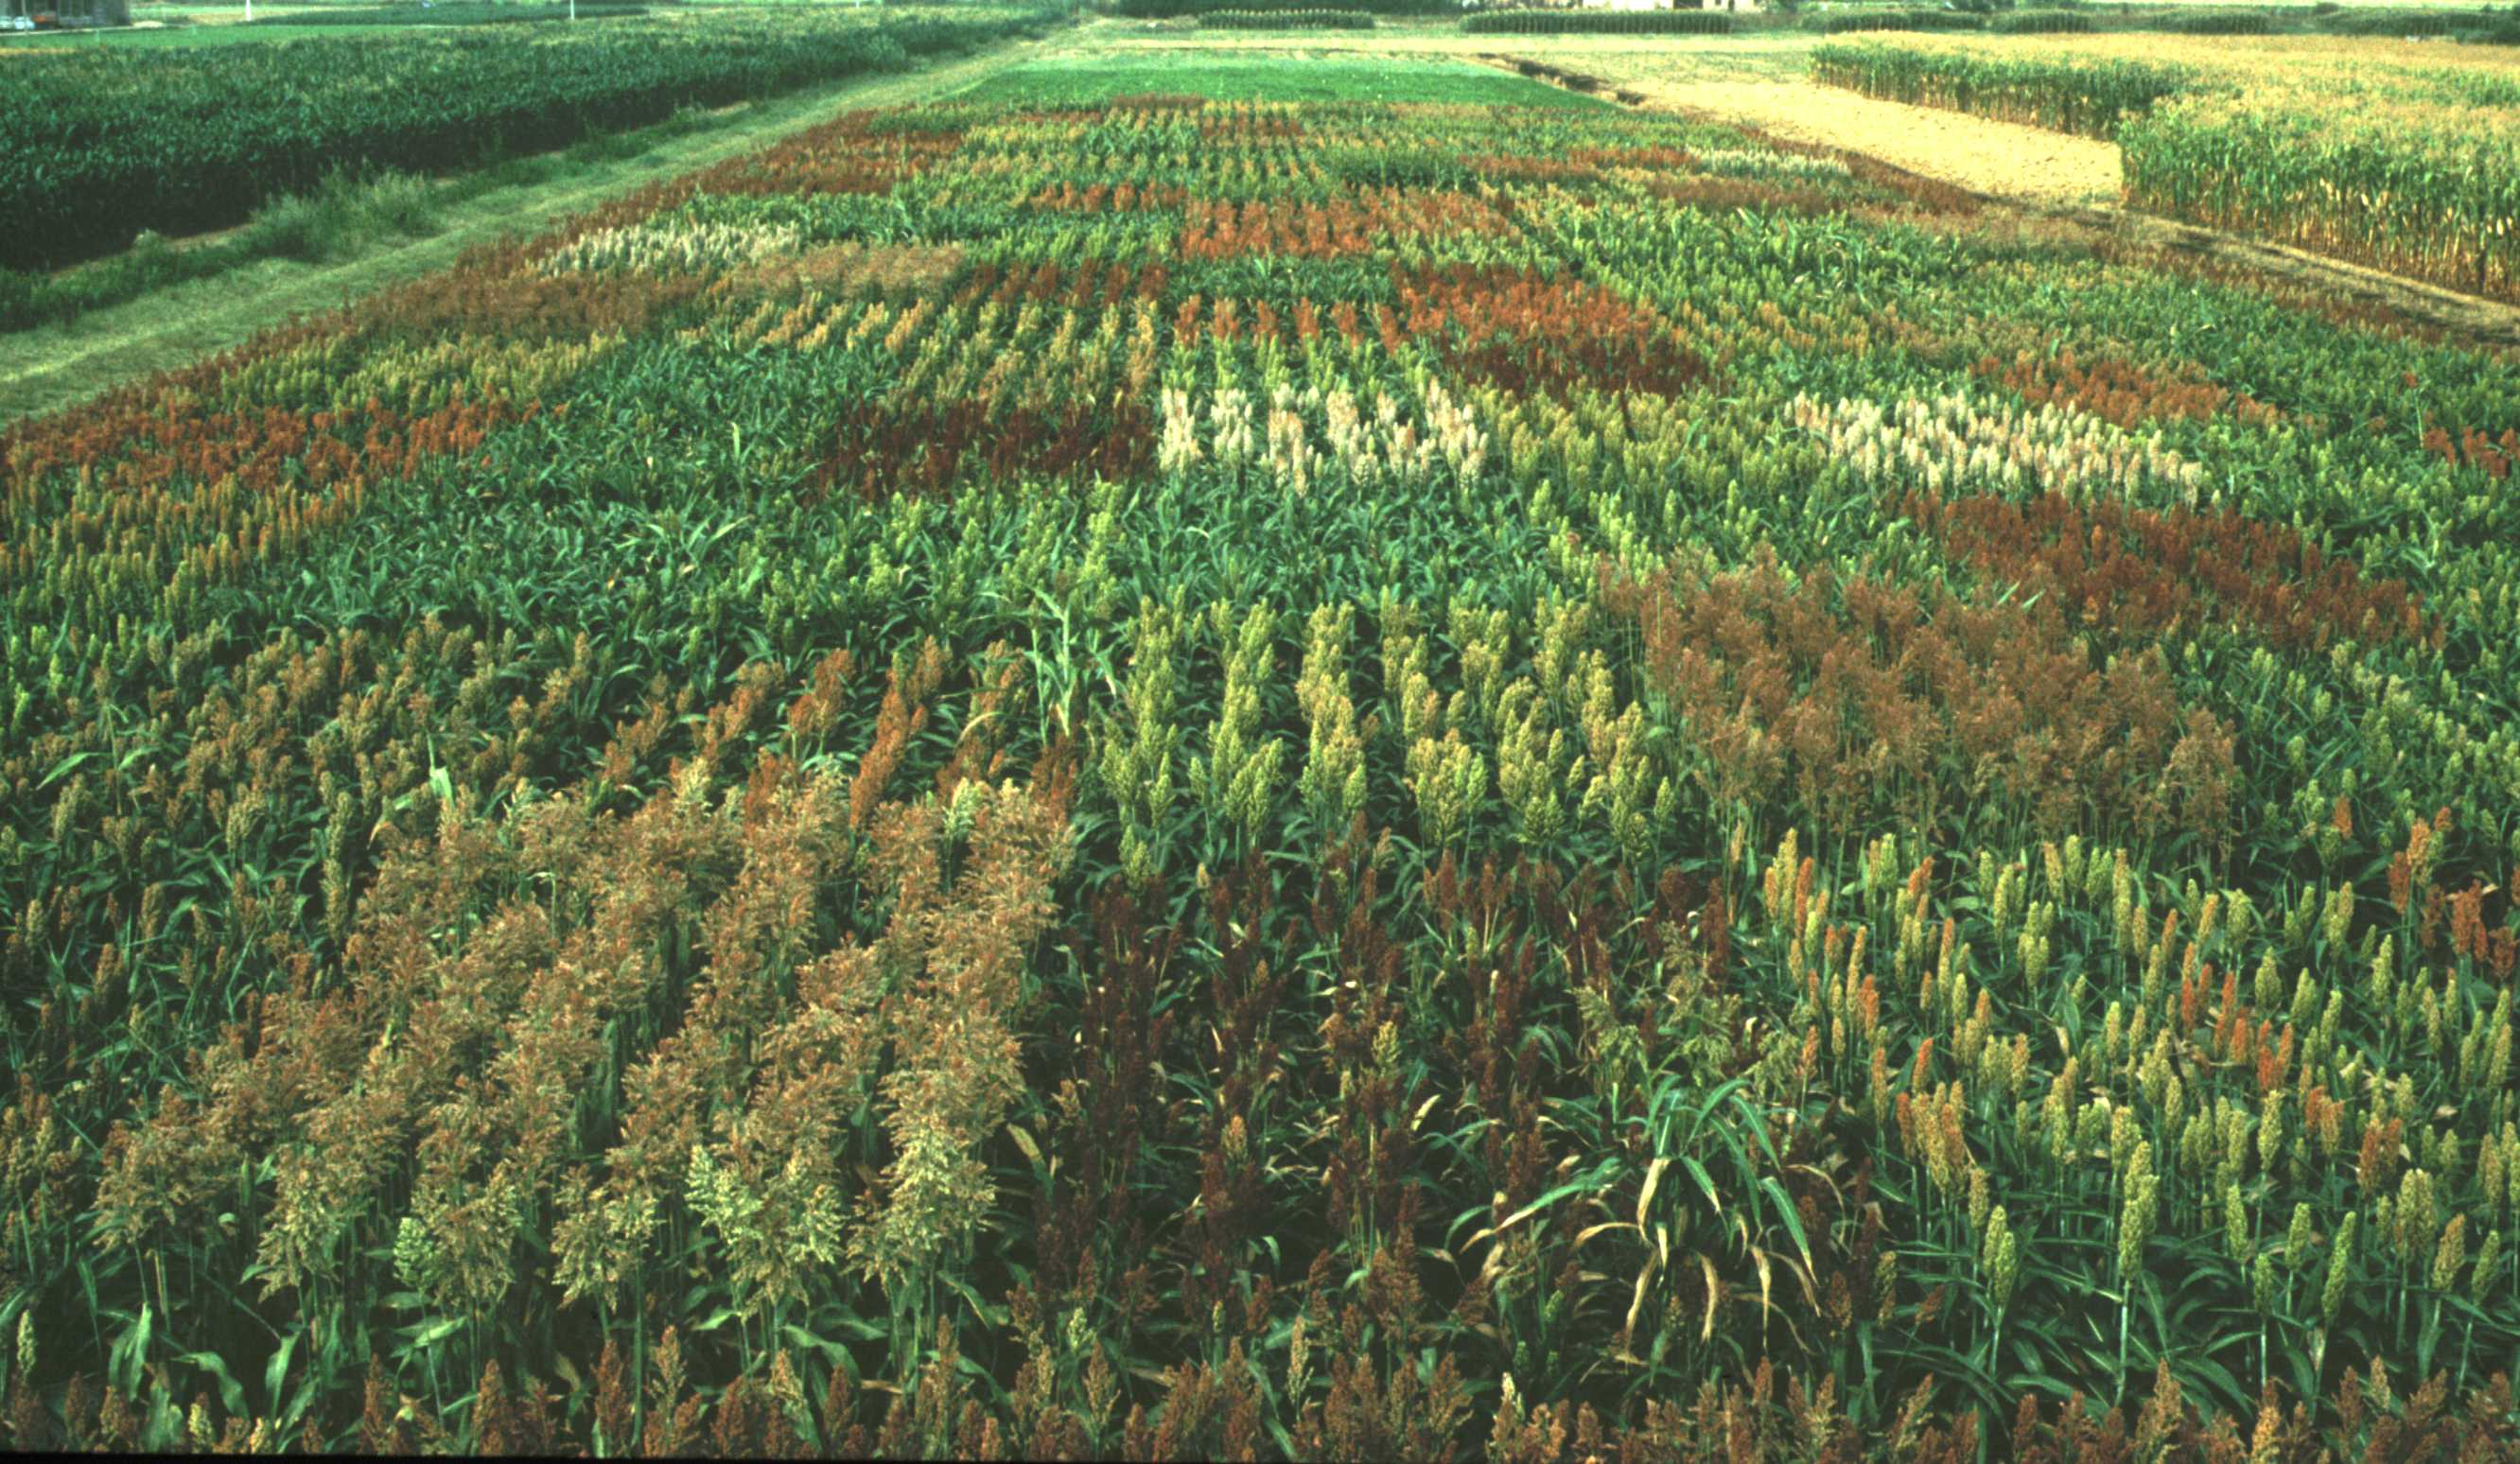
\includegraphics[width=0.9\linewidth]{_images/SorgoProveVarietali} 

}

\caption{A small plot experiment in the field (Ph. D. Alberati)}\label{fig:figName30b}
\end{figure}

Considering the shape, we usually prefer rectangular plots, where the width is equal to a multiple of the width of the available machinery for sowing and harvesting. Plot size must be big enough to accommodate a sufficiently high number of plants; for low density crops (e.g.~maize), 20-40 m\textsuperscript{2} minimum are usually required, while for high density crops (e.g.~wheat or alfalfa) 10-20 m\textsuperscript{2} may suffice. Smaller plots may not produce representative results, but, unless we are planning on-farm experiments, bigger plots can also be disadvantageous, as the plot-to-plot variability is increased. If we have a big field at our disposal, we might prefer to increase the number of replicates, instead of increasing the size of plots.

When selecting plot shape and size we should consider the presence of \textbf{border effects}, that represent an important source of variability. Indeed, plant growing along the plot edges are not in the same conditions as plants in the middle of each plot; for example, they might be more vigorous and productive, because of the lack of competition on one side. Or, they might be affected by, e.g., the carry-over effects of fertilisers and herbicides across neighbouring plots. Border effects need to be minimised by restricting all measurements to the central rows of each plot, while the plants along the edges are omitted. This way, the surface area for harvest is smaller than the total plot surface area, which should be taken into account while designing the experiment.

\hypertarget{number-of-replicates}{%
\subsection{Number of replicates}\label{number-of-replicates}}

For field experiments, the number of replicates is usually set to 3 to 5. A lower number of replicates is not to be recommended, because the experiment becomes very inefficient. On the other hand, a higher number of replicates increases the time and cost requirements and may result in increased soil variability and decreased precision. Once we have selected the number of replicates, the total number of plots is obtained as the product of the number of treatment levels and the number of replicates.

\hypertarget{the-field-map}{%
\subsection{The field map}\label{the-field-map}}

The layout of a field experiment is usually planned in a map (\emph{field map}), showing the lay-out of plots within the field. An example is shown in Figure \ref{fig:figName31}, relating to an experiment with eight treatments and four replicates (32 plots, in total). In order to maximise the homogeneity, we have laid down the plots in eight vertical strips with four plots each. The plots are characterised by a rectangular shape and they are 8 m long and 2 m wide, which makes up a surface area of 16 m\textsuperscript{2}. Around the experiment, we added 24 additional plots, in order to minimise border effects along the edges of the experiment. An arrow pointing towards the North is included, so that we can appropriately orient our map, during the field inspections. All plots are clearly identified by a univocal numbering/coding system.

\begin{figure}

{\centering 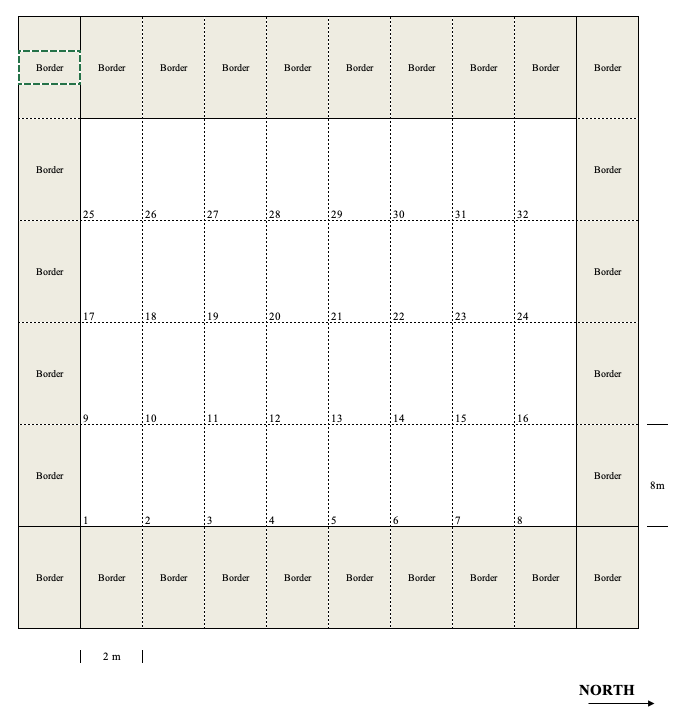
\includegraphics[width=0.9\linewidth]{_images/Mappa1} 

}

\caption{Example of a field map for an experiment with 32 plots}\label{fig:figName31}
\end{figure}

\hypertarget{the-experimental-lay-out}{%
\subsection{The experimental lay-out}\label{the-experimental-lay-out}}

We can use the map to project the allocation of treatments to the units. While the basic principle of randomisation needs to always be followed, the experimental lay-out can be different, according to our organisational needs. The following lay-outs are very common in agriculture, although we will show that they can be used also in experiments of other types.

\hypertarget{completely-randomised-design-cr}{%
\subsubsection{Completely randomised design (CR)}\label{completely-randomised-design-cr}}

With this design, treatments are allocated to plots in a completely randomised fashion, in strict accordance with Fisher's rule. An example is shown in Figure \ref{fig:figName33}, where we have allocated 8 treatments (the letters from A to H) with four replicates to the 32 plots in Figure \ref{fig:figName31}.

\begin{figure}

{\centering 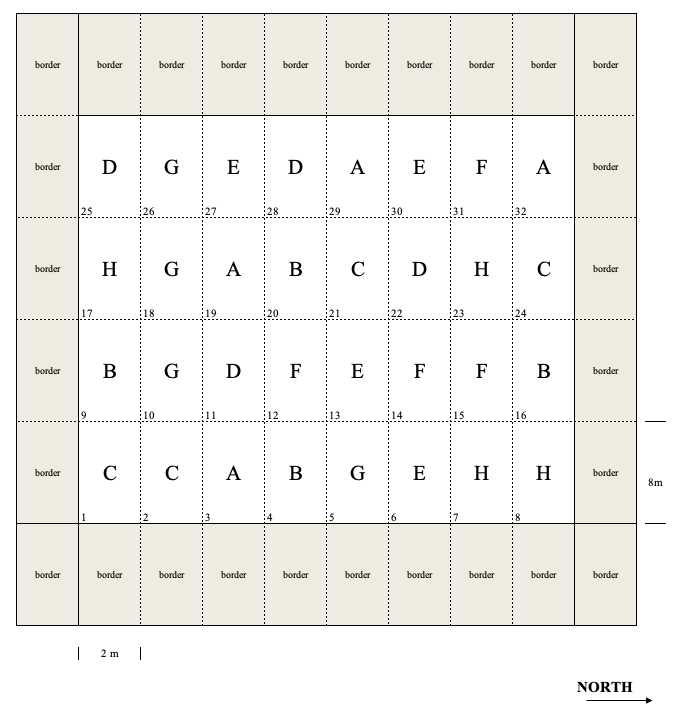
\includegraphics[width=0.97\linewidth]{_images/Mappa1CRD} 

}

\caption{Example of an experiment laid down as a completely randomised design}\label{fig:figName33}
\end{figure}

Such an approach is very simple and always correct, although it has the disadvantage that every possible systematic source of heterogeneity goes unnoticed. For example, let's imagine that, for some reasons, the first three plot columns in Figure \ref{fig:figName33} (plots 1, 2, 3, 9, 10, 11, 17, 18, 19, 25, 26 and 27) are more fertile than all the other columns. In this case, the treatment G is favoured, because three out of four replicates are located in the most fertile part, while the treatment H is penalised, because only one replicate is in that most fertile part.

Therefore, CRDs are very common in laboratory/greenhouse experiments or in field experiments characterised by a high degree of environmental, soil and crop homogeneity.

\hypertarget{randomised-complete-block-design-rcbd}{%
\subsubsection{Randomised complete block design (RCBD)}\label{randomised-complete-block-design-rcbd}}

In RCBDs, the experimental units are divided into homogeneous groups with as many subjects as there are treatments to be allocated. The division is made according to some innate characteristic of subjects, such as age, sex, proximity; for field experiments, we usually exploit some expected fertility gradients. For example, should we expect a left-to-right fertility gradient for the plots in Figure \ref{fig:figName31}, we could divide the experiment in four blocks with two plot columns each (8 plot per each block; block 1 would, e.g., contain the plots 1, 9, 17, 25, 2, 10, 18 e 26). Subsequently, we could randomly allocate the eight treatments to the plots in each block, so that there is one replicate per block. By doing so, no treatment should be penalised/favoured (Figure \ref{fig:figName34})

\begin{figure}

{\centering 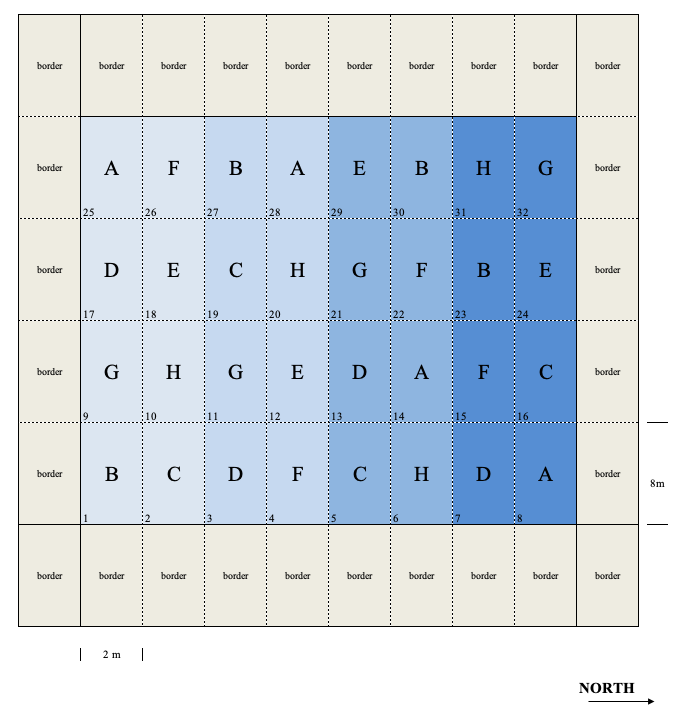
\includegraphics[width=0.97\linewidth]{_images/Mappa1CRBD} 

}

\caption{Example of a completely randomised block design}\label{fig:figName34}
\end{figure}

RCBD is the most common design for field experiments, although it can be used wherever the experimental units can be divided in groups, according to some innate property. In the following chapters we will see that the RCBD is very efficient when the variability across blocks is very big, as a big part of the subject-to-subject variability can be accounted for and removed from the unexplained variation.

\hypertarget{latin-square-design}{%
\subsubsection{Latin square design}\label{latin-square-design}}

In some cases, the experimental units can be grouped according to two innate properties, apart from the experimental treatments. Figure \ref{fig:figName35} shows a design with 4 treatments and four replicates (16 plots in all); if we assume that there are a left-to-right and a bottom-to-top fertility gradients, we can look at the rows and columns as different blocking variables. Therefore, we can allocate the treatments to plots, so that there is one replicate in each row and in each column.

\begin{figure}

{\centering 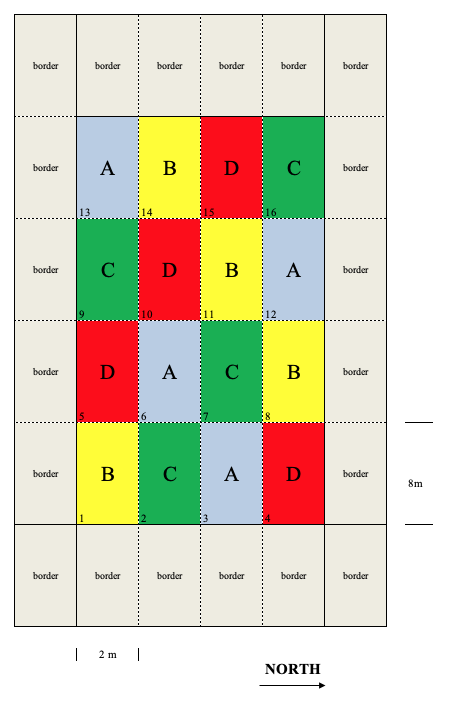
\includegraphics[width=0.7\linewidth]{_images/Mappa2LS} 

}

\caption{Example of a latin square design with four treatments (A, B, C and D) and four replicates. The different colours help identify the four treatments and their allocation to the plots.}\label{fig:figName35}
\end{figure}

Latin square designs are not only useful for field experiments. For example, if we want to test the effect of four different working protocols in the time required to accomplish a certain task, we can use a number of workers as the experimental units. In order to have four replicates, we need 16 workers, to which we allocate the different protocols, according to a CRD or CRBD. We can reduce the number of workers by allowing each worker to use all four protocols, in four subsequent turns. For example, the first worker can use the protocols A, B, C and D, one after the other in a randomised order. By doing so, we only need four workers and the experiment is designed as CRBD, where the worker acts as a blocking factor. The advantage is that possible worker-to-worker differences in proficiency are not confounded with differences between protocols, as all workers use all protocols.

However, we should also consider that workers tend to get tired over time and loose proficiency and, therefore, the protocols used at the beginning of the sequence are favoured with respect to the protocols used later on. We can account for this effect by allocating the protocols in a way that each one is used in all turns; as the consequence, the turn acts as the second blocking factor, as shown in Figure \ref{fig:figName36}. This is, indeed, a latin square design.

\begin{figure}

{\centering 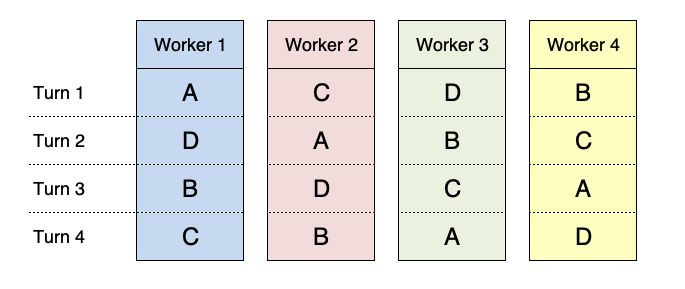
\includegraphics[width=0.9\linewidth]{_images/TurniOperatori} 

}

\caption{Example of a latin square design for the comparison of four working protocols, by using four workers and four turns.}\label{fig:figName36}
\end{figure}

The latin square takes its name from the fact that the number of replicates is equal to the number of treatments and, therefore, the field map consists of a square grid, where each treatment can be found in all rows and all columns (some of you may recognise the basic principle of the Sudoku game\ldots). It is a useful design, as it can account for possible plot-to-plot differences in relation to two blocking factors (rows and columns, or workers and turns), so that the unexplained plot-to-plot differences are minimised. The disadvantage is that the number of replicates must be equal to the number of treatments and, therefore, the latin square can only be used for experiments with few treatments.

\hypertarget{split-plot-and-strip-plot-designs}{%
\subsubsection{Split-plot and strip-plot designs}\label{split-plot-and-strip-plot-designs}}

With factorial experiments we can simply use a CRD or RCBD, by allocating the combinations of all factor levels to the different plots. For example, think about an experiment to compare three types of tillage (minimum tillage = MIN; shallow ploughing = SP; deep ploughing = DP) and two types of chemical weed control methods (broadcast = TOT; in-furrow = PART). With four replicates, the six treatment combinations (MIN-TOT, SP-TOT, DP-TOT, MIN-PART, SP-PART and DP-PART) can be allocated to 24 plots, according to a RCBD, as shown in Figure \ref{fig:figName37}. Please note that we had to allow a wide space between the plots, in order to permit the circulation of tractors and tillage machinery.

\begin{figure}

{\centering 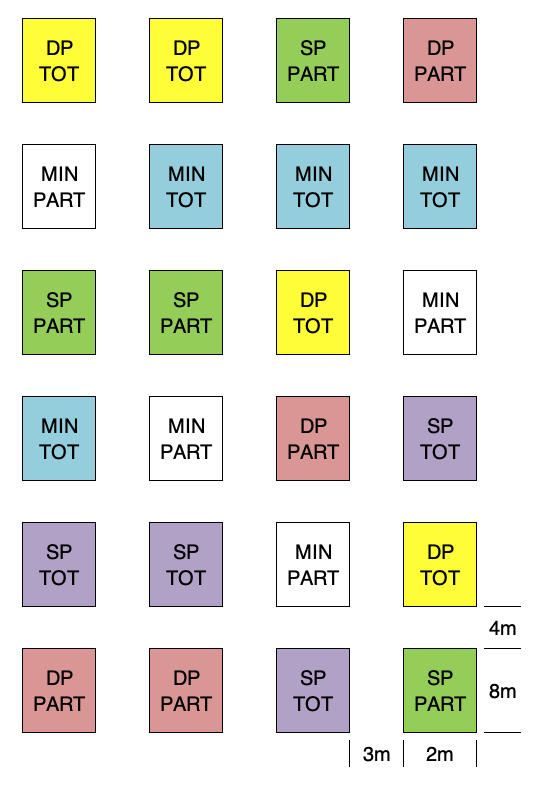
\includegraphics[width=0.75\linewidth]{_images/Mappa3FATT} 

}

\caption{Field map for a two-factor factorial experiment, laid down as RCBD}\label{fig:figName37}
\end{figure}

For those who have some knowledge with field research, it may be obvious that tillage treatments require big plots and a wide space between plots, due to the size of tillage machinery. On the contrary, spraying herbicides may be easily done also on small plots. Therefore, we could think of using big plots to allocate tillage treatments and splitting these big plots into two subplots, to allocate weed control treatments (\textbf{split-plot} design). The example is shown in Figure \ref{fig:figName38}: we note that the allocation of tillage treatments to the 12 main-plots is done according to a RCBD, while the two weed control treatments are randomly allocated to the two sub-plots, within each main-plot.

\begin{figure}

{\centering 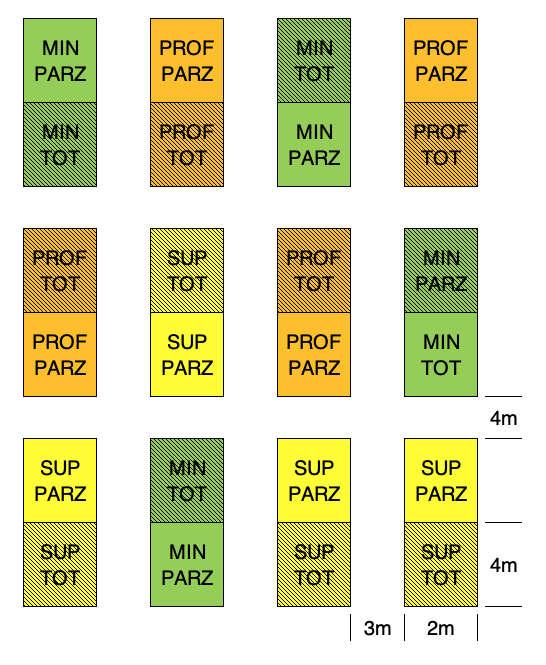
\includegraphics[width=0.75\linewidth]{_images/Mappa3split} 

}

\caption{Same design as in the previous Figure, laid down as split-plot.}\label{fig:figName38}
\end{figure}

An important consequence of split-plot designs is that every main-plot represents a replicate for sub-plot factor levels; indeed, if we look at Figure \ref{fig:figName38}, we see that there are four replicates for each tillage level, but there are 12 replicated sub-plots for each weed control level. Therefore, subplot effects are estimated with higher precision.

As all other designs, split-plot designs are not specific to agriculture experiments and they find their place in many other research topics. In general, they are used whenever:

\begin{enumerate}
\def\labelenumi{\arabic{enumi}.}
\tightlist
\item
  one factor require bigger experimental units, as in the above shown example;
\item
  the levels for one factor are difficult to allocate and it is preferable to manipulate groups of experimental units, instead of a single independent experimental unit. For example, we might be interested in studying the corrosion resistance of steel bars treated with four coatings at three furnace temperatures. This latter factor is hard to change, as it takes a long time to reach a new equilibrium temperature within the furnace. Therefore, once the equilibrium temperature is reached, it is convenient to put four steel bars with each of the four coatings inside the furnace and record their corrosion. We repeat the process at the three temperatures and repeat the whole experiment twice. This is an example of a split-plot experiment, where temperatures are allocated to a furnace (main-plot) and coatings are allocated the steel bars (sub-plots).
\end{enumerate}

A useful variant of the split plot is used when the treatments are allocated in strips (\textbf{strip-plot} designs), as shown in Figure \ref{fig:figName39}. This map refers to an experiment where three crops were sown 40 days after a herbicide treatment, in order to assess possible phytotoxicity effects relating to an excessive persistence of herbicide residues. We see that each block is organised with three rows and two columns: the three crops were sown along the rows and the two herbicide treatments (rimsulfuron and the untreated control) were allocated along the columns. The combinations are, consequently, allocated to subplots. In this design, we have three types of plots: the row-plots, the column-plots and the subplots; the advantage is that the allocation of treatments is rather quick.

\begin{figure}

{\centering 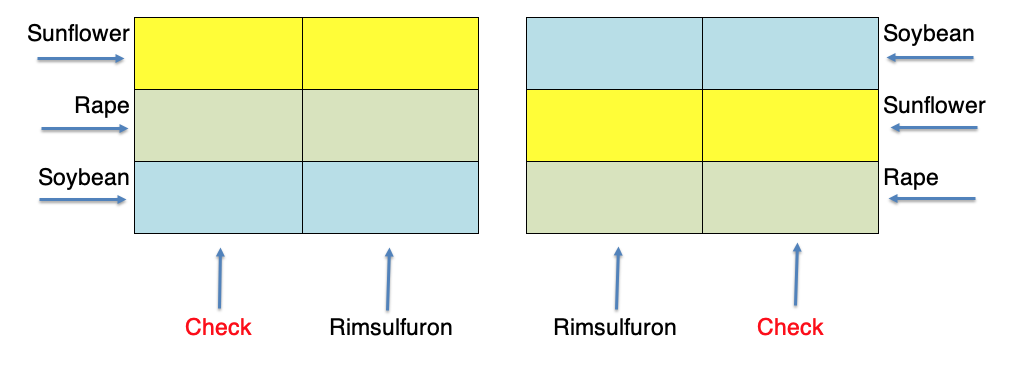
\includegraphics[width=0.75\linewidth]{_images/StripPlotEng} 

}

\caption{Same design as in the previous Figure, laid down as strip-plot.}\label{fig:figName39}
\end{figure}

\hypertarget{conclusions-1}{%
\section{Conclusions}\label{conclusions-1}}

In this chapter we have seen the fundamental elements of a research and we have also seen how those elements, considering the three fundamental characteristics of control, replication and randomisation, can be joined together to set-up valid experiments in the field. We have also seen that the different types of designs are commonly used also for laboratory experiments or other types of experiments outside agriculture.

\begin{center}\rule{0.5\linewidth}{0.5pt}\end{center}

\hypertarget{further-readings-1}{%
\section{Further readings}\label{further-readings-1}}

\begin{enumerate}
\def\labelenumi{\arabic{enumi}.}
\tightlist
\item
  Cochran, W.G., Cox, G.M., 1950. Experimental design. John Wiley \& Sons, Inc., Books.
\item
  Daniel, J. 2011. Sampling Essentials: Practical Guidelines for Making Sampling Choices. USA: SAGE.
\item
  LeClerg, E.L., Leonard, W.H., Clark, A.G., 1962. Field Plot Technique. Burgess Publishing Company, Books.
\item
  Jones, B., Nachtsheim, C.J., 2009. Split plot designs: what, why and how. Journal of Quality Technology 41, 340--361.
\end{enumerate}

\hypertarget{describing-the-observations}{%
\chapter{Describing the observations}\label{describing-the-observations}}

The final outcome of every manipulative/comparative experiment is a \textbf{dataset}, consisting of a set of measures/observations taken on several experimental subjects, in relation to one or more properties (e.g., height, weight, concentration, sex, color). We have seen that the list of values for one of those properties is called a variable; our first task is to describe that variable, by using the most appropriate descriptive stats. In this respect, the different types of variables (see Chapter 2) will require different approaches, as we will see in this chapter.

\hypertarget{quantitative-data}{%
\section{Quantitative data}\label{quantitative-data}}

For a quantitative variable, we need to describe:

\begin{enumerate}
\def\labelenumi{\arabic{enumi}.}
\tightlist
\item
  location
\item
  spread
\item
  shape
\end{enumerate}

The three statistics respond, respectively, to the following questions: (1) where are the values located, along the measurement scale? (2) how close are the values to one another? (3) are the values symmetrically distributed around the central value, or are they skewed to the right or to the left?

In this chapter, we will only consider the statistics of location and spread, as the statistics of shape are not commonly reported in agriculture and biology.

\hypertarget{statistics-of-location}{%
\subsection{Statistics of location}\label{statistics-of-location}}

The most widely known statistic of location is the \textbf{mean}, that is obtained as the sum of data, divided by the number of values:

\[\mu = \frac{\sum\limits_{i = 1}^n x_i}{n}\]

For example, let us consider the following variable, listing the heights of four maize plants: \(x = [178, 175, 158, 153]\)

The mean is easily calculated as:

\[\mu = \frac{178 + 175 + 158 + 153}{4} = 166\]

The mean can be regarded as the central value in terms of Euclidean distances; indeed, by definition, the sum of the Euclidean distances between the values and the group mean is always zero. In other words, the values above the mean and those below the mean, on average, are equally distant from the mean. That does not imply that the number of values above the mean is the same as the number of values below the mean. For example, if we look at the following values:

1 - 4 - 7 - 9 - 10

we see that the mean is 6.2. If we change the highest value into 100, the new mean is moved upwards to 24.2 and it is no longer in central positioning, with respect to the sorted list of data values.

Another important statistic of location is the \textbf{median}, i.e.~the central value in a sorted variable. The calculation is easy: first of all, we sort the values in increasing order. If the number of values is odd, the median is given by the value in the \((n + 1)/2\) position (\(n\) is the number of values). Otherwise, if the number of values is even, we take the two values in the \(n/2\) and \(n/2 + 1\) positions and average them.

The median is always the central value in terms of positioning, i.e., the number of values above the median is always equal to the number of values below the median. For example if we take the same values as above (1 - 4 - 7 - 9 - 10), the median is equal to 7 and it is not affected when we change the highest value into 100. Considering that extreme values (very high or very low) are usually known as \emph{outliers}, we say that the median is more \textbf{robust} than the mean with respect to outliers.

\hypertarget{statistics-of-spread}{%
\subsection{Statistics of spread}\label{statistics-of-spread}}

Knowing the location of a variable is not enough for our purpose as we miss an important information: how close are the values to the mean? The simplest statistic to express the spread is the \textbf{range}, that is the difference between the highest and lowest value. This is a very rough indicator, though, as it is extremely sensitive to outliers.

In the presence of a few outliers, the median is used as a statistic of location and, in that case, it can be associated, as a statistic of spread, to the interval defined by the 25\textsuperscript{th} and 75\textsuperscript{th} percentiles. In general, the \textbf{percentiles}, are the values below which a given percentage of observations falls. More specifically, the 25\textsuperscript{th} percentile is the value below which 25\% of the observations falls and the 75\textsuperscript{th} percentile is the value below which 75\% of the observations falls (you may have understood that the median corresponds to the 50\textsuperscript{th} percentile). The interval between the 25\textsuperscript{th} and 75\textsuperscript{th} percentile, consequently, contains 50\% of all the observed values and, therefore, it is a good statistic of spread.

If we prefer to use the mean as a statistic of location, we can use several other important statistics od spread; the first one, in order of calculation, is the \textbf{deviance}, that is also known as the \textbf{sum of squares}. It is the sum of squared differences between each value and the mean:

\[SS = \sum\limits_{i = 1}^n {(x_i  - \mu)^2 }\]

In the above expression, the amounts \(x_i - \mu\) (differences between each value and the group mean) are known as \textbf{residuals}. For our sample, the deviance is:

\[SS = \left(178 - 166 \right)^2 + \left(175 - 166 \right)^2 + \left(158 - 166 \right)^2  + \left(153 - 166 \right)^2= 458\]

A high deviance corresponds to a high spread; however, we can have a high deviance also when we have low spread and a lot of values. Therefore, the deviance should not be used to compare the spread of two groups with different sizes. Another problem with the deviance is that the measurement unit is also squared with respect to the mean: for our example, if the original variable (height) is measured in cm, the deviance is measured in cm\textsuperscript{2}, which is not very logical.

A second important measure of spread is the \textbf{variance}, that is usually obtained dividing the deviance by the number of observations minus one:

\[\sigma^2  = \frac{SS}{n - 1}\]

For our group:

\[\sigma^2  = \frac{458}{3} = 152.67\]

The variance can be used to compare the spread of two groups with different sizes, but the measurement unit is still squared, with respect to the original variable.

The most important measure of spread is the \textbf{standard deviation}, that is the square root of the variance:

\[\sigma = \sqrt{\sigma^2} = \sqrt{152.67} = 12.36\]

The measurement unit is the same as the data and, for this reason, the standard deviation is the most important statistic of spread and it is usually associated to the mean to summarise a set of measurements. In particular, the interval \(l = \mu \pm \sigma\) is often used to describe the \textbf{absolute uncertainty} of replicated measurements.

Sometimes, the standard deviation is expressed as a percentage of the mean (\textbf{coefficient of variability}), which is often used to describe the \textbf{relative uncertainty} of measurement instruments:

\[CV = \frac{\sigma }{\mu } \times 100\]

\hypertarget{summing-the-uncertainty}{%
\subsection{Summing the uncertainty}\label{summing-the-uncertainty}}

In some cases, we measure two quantities and sum them to obtain a derived quantity. For example, we might have made replicated measurements to determine the sucrose content in a certain growth substrate, that was equal to \(22 \pm 2\) (mean and standard deviation). Likewise, another independent set of measures showed that the fructose content in the same substrate was \(14 \pm 3\). Total sugar content is equal to the sum of \(22 + 14 = 36\). The absolute uncertainty for the sum is given by the square root of the sum of the squared absolute uncertainties, that is \(36 \pm \sqrt{4 + 9}\). The absolute uncertainty for a difference is calculated in the very same way.

\hypertarget{relationship-between-quantitative-variables}{%
\subsection{Relationship between quantitative variables}\label{relationship-between-quantitative-variables}}

Very frequently, we may have recorded, on each subject, two, or more, quantitative traits, so that, in the end, we have two, or more, response variables. We might be interested in assessing whether, for each pair of variables, when one changes, the other one changes, too (\textbf{joint variation}). The \emph{Pearson correlation coefficient} is a measure of joint variation and it is equal to the codeviance of the two variables divided by the square root of the product of their deviances:

\[r = \frac{ \sum_{i=1}^{n}(x_i - \mu_x)(y_i-\mu_y) }{\sqrt{\sum_{i=1}^{n}(x_i-\mu_x)^2 \sum_{i=1}^{n}(y_i-\mu_y)^2}}\]

We know about the deviance, already. The codeviance is a statistic that consists of the product of the residuals for the two variables: it is positive, when the residuals for the two variables have the same signs, otherwise it is negative. Consequently, the \(r\) coefficient ranges from \(+1\) to \(-1\): a value of \(+1\) implies that, when \(x\) increases, \(y\) increases by a proportional amount, so that the points on a scatterplot lie on a straight line, with positive slope. On the other hand, a value of \(-1\) implies that when \(x\) increases, \(y\) decreases by a proportional amount, so that the points on a scatterplot lie on a straight line, with negative slope. A value of 0 indicates that there is no joint variability, while intermediate values indicate a more or less high degree of joint variability, although the points on a scatterplot do not exactly lie on a straight line (Figure 3.1).

\begin{figure}

{\centering 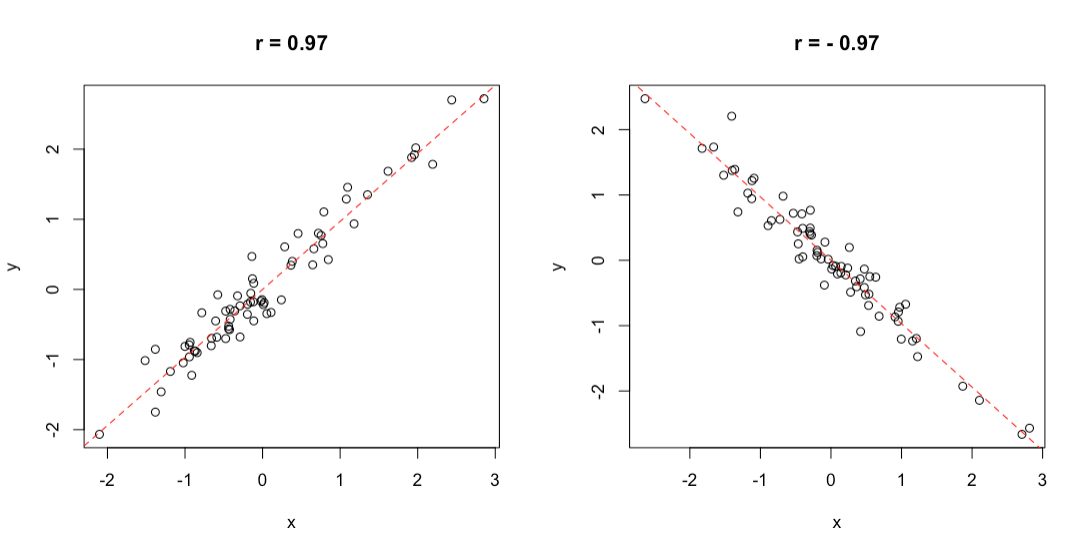
\includegraphics[width=0.75\linewidth]{_images/CorrelationExample} 

}

\caption{Example of positive (left) and negative (right) correlation}\label{fig:figName311}
\end{figure}

For example, if we have measured the oil content in sunflower seeds by using two different methods, we may be interested in describing the correlation between the results of the two methods. The observed data are shown in the box below.

\begin{Shaded}
\begin{Highlighting}[]
\NormalTok{A }\OtherTok{\textless{}{-}} \FunctionTok{c}\NormalTok{(}\DecValTok{45}\NormalTok{, }\DecValTok{47}\NormalTok{, }\DecValTok{49}\NormalTok{, }\DecValTok{51}\NormalTok{, }\DecValTok{44}\NormalTok{, }\DecValTok{37}\NormalTok{, }\DecValTok{48}\NormalTok{, }\DecValTok{42}\NormalTok{, }\DecValTok{53}\NormalTok{)}
\NormalTok{B }\OtherTok{\textless{}{-}} \FunctionTok{c}\NormalTok{(}\DecValTok{44}\NormalTok{, }\DecValTok{44}\NormalTok{, }\DecValTok{49}\NormalTok{, }\DecValTok{53}\NormalTok{, }\DecValTok{48}\NormalTok{, }\DecValTok{34}\NormalTok{, }\DecValTok{47}\NormalTok{, }\DecValTok{39}\NormalTok{, }\DecValTok{51}\NormalTok{)}
\end{Highlighting}
\end{Shaded}

In order to calculate the correlation coefficient, we need to organise our calculations as follows:

\begin{enumerate}
\def\labelenumi{\arabic{enumi}.}
\tightlist
\item
  calculate the residuals for A (\(z_A\))
\item
  calculate the residuals for B (\(z_B\))
\item
  calculate the deviances and codeviance
\end{enumerate}

First of all, we calculate the two means, that are, respectively, 46.22 and 45.44. Secondly, we can calculate the residuals for both variables, as shown in Table 3.1. From the residuals, we can calculate the deviances and the codeviance, by using the equation above.

\begin{table}

\caption{\label{tab:unnamed-chunk-3}Example of the hand calculations that are used to calculate the correlation coefficient}
\centering
\begin{tabular}[t]{rrrrrrr}
\toprule
A & B & \$z\_A\$ & \$z\_B\$ & \$z\_A\textasciicircum{}2\$ & \$z\_B\textasciicircum{}2\$ & \$z\_A \textbackslash{}times z\_B\$\\
\midrule
45 & 44 & -1.222 & -1.444 & 1.494 & 2.086 & 1.765\\
47 & 44 & 0.778 & -1.444 & 0.605 & 2.086 & -1.123\\
49 & 49 & 2.778 & 3.556 & 7.716 & 12.642 & 9.877\\
51 & 53 & 4.778 & 7.556 & 22.827 & 57.086 & 36.099\\
44 & 48 & -2.222 & 2.556 & 4.938 & 6.531 & -5.679\\
\addlinespace
37 & 34 & -9.222 & -11.444 & 85.049 & 130.975 & 105.543\\
48 & 47 & 1.778 & 1.556 & 3.160 & 2.420 & 2.765\\
42 & 39 & -4.222 & -6.444 & 17.827 & 41.531 & 27.210\\
53 & 51 & 6.778 & 5.556 & 45.938 & 30.864 & 37.654\\
\bottomrule
\end{tabular}
\end{table}

The deviances for \(A\) and \(B\) are, respectively, 189.55 and 286.22, while the codeviance is 214.11. Accordingly, the correlation coefficient is:

\[r = \frac{214.11}{\sqrt{189.55 \times 286.22}} = 0.919\]

It is close to 1, so we conclude that there was quite a good agreement between the two methods.

\hypertarget{nominal-data}{%
\section{Nominal data}\label{nominal-data}}

\hypertarget{distributions-of-frequencies}{%
\subsection{Distributions of frequencies}\label{distributions-of-frequencies}}

With nominal data, we can only assign the individuals to one of a number of categories. In the end, the only description we can give of such a dataset is based on the counts (\textbf{absolute frequencies}) of individuals in each category, producing the so called \textbf{distribution of frequencies}.

As an example of nominal data we can take the `mtcars' dataset, that was extracted from the 1974 Motor Trend US magazine and comprises 32 old automobiles. The dataset is available in R and we show part of it in table 3.2.

\begin{table}

\caption{\label{tab:unnamed-chunk-4}Dataset 'mtcars' in R, representing the characteristics of 32 old automobiles; 'cs' is the type of engine and 'gear' is the number of forward gears. More detail is given in the text.}
\centering
\begin{tabular}[t]{lrr}
\toprule
  & vs & gear\\
\midrule
Mazda RX4 & 0 & 4\\
Mazda RX4 Wag & 0 & 4\\
Datsun 710 & 1 & 4\\
Hornet 4 Drive & 1 & 3\\
Hornet Sportabout & 0 & 3\\
\addlinespace
Valiant & 1 & 3\\
Duster 360 & 0 & 3\\
Merc 240D & 1 & 4\\
Merc 230 & 1 & 4\\
Merc 280 & 1 & 4\\
\addlinespace
Merc 280C & 1 & 4\\
Merc 450SE & 0 & 3\\
Merc 450SL & 0 & 3\\
Merc 450SLC & 0 & 3\\
Cadillac Fleetwood & 0 & 3\\
\addlinespace
Lincoln Continental & 0 & 3\\
Chrysler Imperial & 0 & 3\\
Fiat 128 & 1 & 4\\
Honda Civic & 1 & 4\\
Toyota Corolla & 1 & 4\\
\addlinespace
Toyota Corona & 1 & 3\\
Dodge Challenger & 0 & 3\\
AMC Javelin & 0 & 3\\
Camaro Z28 & 0 & 3\\
Pontiac Firebird & 0 & 3\\
\addlinespace
Fiat X1-9 & 1 & 4\\
Porsche 914-2 & 0 & 5\\
Lotus Europa & 1 & 5\\
Ford Pantera L & 0 & 5\\
Ferrari Dino & 0 & 5\\
\addlinespace
Maserati Bora & 0 & 5\\
Volvo 142E & 1 & 4\\
\bottomrule
\end{tabular}
\end{table}

The variable `vs' in `mtcars' takes the values 0 for V-shaped engine and 1 for straight engine. Obviously, the two values 0 and 1 are just used to name the two categories and the resulting variable is purely nominal. The absolute frequencies of cars in the two categories are, respectively 18 and 14 and they are easily obtained by a counting process.

We can also calculate the relative frequencies, dividing the absolute frequencies by the total number of observations. These frequencies are, respectively, 0.5625 and 0.4375.

If we consider a variable where the classes can be logically ordered, we can also calculate the \textbf{cumulative frequencies}, by summing up the frequency for one class with the frequencies for all previous classes. As an example we take the `gear' variable in the `mtcars' dataset, showing the number of forward gears for each car. We can easily see that 15 cars have 3 gears and 27 cars have 4 gears or less.

In some circumstances, it may be convenient to `bin' a continuous variable into a set of intervals. For example, if we have recorded the ages of a big group of people, we can divide the scale into intervals of five years (e.g., from 10 to 15, from 15 to 20 and so on) and, eventually, assign each individual to the appropriate age class. Such a technique is called \textbf{binning} or \textbf{bucketing} and we will see an example later on in this chapter.

\hypertarget{descriptive-stats-for-distributions-of-frequencies}{%
\subsection{Descriptive stats for distributions of frequencies}\label{descriptive-stats-for-distributions-of-frequencies}}

For categorical data, we can retrieve the \textbf{mode}, which is the class with the highest frequency. For ordinal data, wherever distances between classes are meaningful, and for discrete data, we can also calculate the median and other percentiles, as well as the mean and other statistics of spread (e.g., variance, standard deviation). The mean is calculated as:

\[ \mu = \frac{\sum\limits_{i = 1}^n f_i x_i}{\sum\limits_{i = 1}^n f_i}\]

where \(x_i\) is the value for the i-th class, and \(f_i\) is the frequency for the same class. Likewise, the deviance, is calculated as:

\[ SS = \sum\limits_{i = 1}^n f_i (x_i - \mu)^2 \]

For example, considerin the `gear' variable in Table 3.2, the average number of forward gears is:

\[\frac{ 15 \times 3 + 12 \times 4 + 5 \times 5}{15 + 12 + 5} = 3.6875\]

while the deviance is:

\[SS = 15 \times (3 - 3.6875)^2 + 12 \times (4 - 3.6875)^2 + 5 \times (5 - 3.l875)^2 = 16.875\]

With interval data (binned data), descriptive statistics should be calculated by using the raw data, if they are available. If they are not, we can use the frequency distribution obtained from binning, by assigning to each individual the central value of the interval class to which it belongs. As an example, we can consider the distribution of frequencies in Table 3.3, relating to the time (in minutes) taken to complete a statistic assignment for a group of students in biotechnology. We can see that the mean is equal to:

\[ \frac{7.5 \times 1 + 12.5 \times 4 + 17.5 \times 3 + 22.5 \times 2}{10} = 15.5\]

\begin{table}

\caption{\label{tab:unnamed-chunk-5}Distribution of frequency for the time (in minutes) taken to complete a statistic assignment for a group of students in biotechnology}
\centering
\begin{tabular}[t]{ccc}
\toprule
Time interval & Central value & Count\\
\midrule
5 - 10 & 7.5 & 1\\
10 - 15 & 12.5 & 4\\
15 - 20 & 17.5 & 3\\
20 - 25 & 22.5 & 2\\
\bottomrule
\end{tabular}
\end{table}

The calculation of the deviance is left as an exercise.

\hypertarget{contingency-tables}{%
\subsection{Contingency tables}\label{contingency-tables}}

When we have more than one cataegorical variable, we can summarise the distribution of frequency by using two-way tables, usually known as \textbf{contingency tables} or crosstabs. For example, we can consider the `HairEyeColor' dataset, in the `datasets' package, which is part of the base R installation. It shows the contingency tables of hair and eye color in 592 statistics students, depending on sex; both characters are expressed in four classes, i.e.~black, brown, red and blond hair and brown, blue, hazel and green eyes. Considering females, the contingency table is reported in Table 3.4 and it is augmented with row and column sums (see later).

\begin{table}

\caption{\label{tab:unnamed-chunk-6}Distribution of hair and eye color for 313 female statistics students, augmented with row and column sums. Dataset taken from R package 'datasets'}
\centering
\begin{tabular}[t]{lccccc}
\toprule
  & Brown eye & Blue eye & Hazel eye & Green eye & ROW SUMS\\
\midrule
Black hair & 36 & 9 & 5 & 2 & 52\\
Brown hair & 66 & 34 & 29 & 14 & 143\\
Red hair & 16 & 7 & 7 & 7 & 37\\
Blond hair & 4 & 64 & 5 & 8 & 81\\
COLUMN SUMS & 122 & 114 & 46 & 31 & 313\\
\bottomrule
\end{tabular}
\end{table}

\hypertarget{independence}{%
\subsection{Independence}\label{independence}}

With a contingency table, we may be interested in assessing whether the two variables show some sort of dependency relationship. In the previous example, is there any relationship between the color of the eyes and the color of the hair? If not, we say that the two variables are independent. Independency is assessed by using the \(\chi^2\) statistic.

As the first step, we need to calculate the \emph{marginal frequencies}, i.e.~the sums of frequencies by row and by column (please note that the entries of a contingency table are called \emph{joint frequencies}). These sums are reported in Table 3.4.

Let's consider black hair: in total there are 52 women with black air, that is \(52/313 \times 100 = 16.6\)\% of the total. If the two characters were independent, the above proportion should not change, depending on the color of eyes. For example, we have 122 women with brown eyes and 16.6\% of those should be black haired, which makes up an expected value of 20.26837 black haired and brown eyed women (much lower than the observed 36). Another example: the expected value of blue eyed and black haired women is \(114 \times 0.166 = 18.9\) (much higher than the observed). A third example may be useful: in total, there is \(143/313 = 45.7\)\% of brown haired women and, in case of independence, we would expect \(46 \times 0.457 = 21.02\) brown haired and hazel eyed woman. Keeping on with the calculations, we could derive a table of expected frequency, in the case of complete independence between the two characters. All the expected values in case of independency are reported in Table 3.5.

\begin{table}

\caption{\label{tab:unnamed-chunk-8}Expected values of hair and eye color for 313 female statistics students, augmented with row and column sums. Expectations assume total lack of dependency between the two variables.}
\centering
\begin{tabular}[t]{lccccc}
\toprule
  & Brown eye & Blue eye & Hazel eye & Green eye & ROW SUMS\\
\midrule
Black hair & 20.26837 & 18.93930 & 7.642173 & 5.150160 & 52\\
Brown hair & 55.73802 & 52.08307 & 21.015974 & 14.162939 & 143\\
Red hair & 14.42173 & 13.47604 & 5.437700 & 3.664537 & 37\\
Blond hair & 31.57189 & 29.50160 & 11.904153 & 8.022364 & 81\\
COLUMN SUMS & 122.00000 & 114.00000 & 46.000000 & 31.000000 & 313\\
\bottomrule
\end{tabular}
\end{table}

The observed (table 3.4) and expected (Table 3.5) values are different, which might indicate a some sort of relationship between the two variables; for example, having red hair might imply that we are more likely to have eyes of a certain color. In order to quantify the discrepancy between the two tables, we calculate the \(\chi^2\) stat, that is:

\[\chi ^2  = \sum \left[ \frac{\left( {f_o  - f_e } \right)^2 }{f_e } \right]\]

where \(f_o\) are the observed frequencies and \(f_e\) are the expected frequencies. For example, for the first value we have:

\[\chi^2_1  = \left[ \frac{\left( {36  - 20.26837 } \right)^2 }{20.26837 } \right]\]

In all, we should calculate 16 ratios and sum them to each other. The final \(\chi^2\) value should be equal to 0 in case of independence and it should increase as the relationship between the two variables increases, up to:

\[\max \chi ^2  = n \cdot \min (r - 1,\,c - 1)\]

i.e.~the product between the number of subjects (\(n\)) and the minimum value between the number of rows minus one and the number of columns minus one (in our case, it is \(313 \times 3 = 939\)).

The observed value is 106.66 and it suggests that the two variables are not independent.

\hypertarget{descriptive-stats-with-r}{%
\section{Descriptive stats with R}\label{descriptive-stats-with-r}}

Before reading this part, please make sure that you already have some basic knowledge about the R environment. Otherwise, please go and read the Appendix 1 to this book.

Relating to quantitative variables, we can use the dataset `heights.csv,' that is available in an online repository and refers to the height of 20 maize plants. In R, the mean is calculated by the function \texttt{mean()}, as shown in the box below.

\begin{Shaded}
\begin{Highlighting}[]
\NormalTok{filePath }\OtherTok{\textless{}{-}} \StringTok{"https://www.casaonofri.it/\_datasets/heights.csv"}
\NormalTok{dataset }\OtherTok{\textless{}{-}} \FunctionTok{read.csv}\NormalTok{(filePath, }\AttributeTok{header =}\NormalTok{ T)}
\FunctionTok{mean}\NormalTok{(dataset}\SpecialCharTok{$}\NormalTok{height)}
\DocumentationTok{\#\# [1] 164}
\end{Highlighting}
\end{Shaded}

The median is obtained by using the function \texttt{median()}:

\begin{Shaded}
\begin{Highlighting}[]
\FunctionTok{median}\NormalTok{(dataset}\SpecialCharTok{$}\NormalTok{height)}
\DocumentationTok{\#\# [1] 162.5}
\end{Highlighting}
\end{Shaded}

The other percentiles are calculated with the function \texttt{quantile()}, passing the selected probabilities as fractions in a vector:

\begin{Shaded}
\begin{Highlighting}[]
\FunctionTok{quantile}\NormalTok{(dataset}\SpecialCharTok{$}\NormalTok{height, }\AttributeTok{probs =} \FunctionTok{c}\NormalTok{(}\FloatTok{0.25}\NormalTok{, }\FloatTok{0.75}\NormalTok{))}
\DocumentationTok{\#\#    25\%    75\% }
\DocumentationTok{\#\# 152.75 174.25}
\end{Highlighting}
\end{Shaded}

The deviance function is not immediately available in R and we should resort to using the following expression:

\begin{Shaded}
\begin{Highlighting}[]
\FunctionTok{sum}\NormalTok{( (dataset}\SpecialCharTok{$}\NormalTok{height }\SpecialCharTok{{-}} \FunctionTok{mean}\NormalTok{(dataset}\SpecialCharTok{$}\NormalTok{height))}\SpecialCharTok{\^{}}\DecValTok{2}\NormalTok{ )}
\DocumentationTok{\#\# [1] 4050}
\end{Highlighting}
\end{Shaded}

The other variability stats are straightforward to obtain, as well as the correlation coefficient:

\begin{Shaded}
\begin{Highlighting}[]
\CommentTok{\# Variance and standard deviation}
\FunctionTok{var}\NormalTok{(dataset}\SpecialCharTok{$}\NormalTok{height)}
\DocumentationTok{\#\# [1] 213.1579}
\FunctionTok{sd}\NormalTok{(dataset}\SpecialCharTok{$}\NormalTok{height)}
\DocumentationTok{\#\# [1] 14.59993}
\CommentTok{\# Coefficient of variability}
\FunctionTok{sd}\NormalTok{(dataset}\SpecialCharTok{$}\NormalTok{height)}\SpecialCharTok{/}\FunctionTok{mean}\NormalTok{(dataset}\SpecialCharTok{$}\NormalTok{height) }\SpecialCharTok{*} \DecValTok{100}
\DocumentationTok{\#\# [1] 8.902395}
\CommentTok{\# Correlation}
\FunctionTok{cor}\NormalTok{(A, B)}
\DocumentationTok{\#\# [1] 0.9192196}
\end{Highlighting}
\end{Shaded}

We have just listed some of the main stats that can be used to describe the properties of a quaantitative variable. In our research work we usually deal with several groups of observations, each one including the different replicates of one of a series of experimental treatments. Therefore, we need to be able to obtain the descriptive stats for all groups at the same time. The very basic method to do this, is by using the function \texttt{tapply()}, which takes three arguments, i.e.~the vector of observations, the vector of groups and the function to be calculated by groups. The vector of groups is the typical accessory variable, which labels the observations according to the group they belong to.

\begin{Shaded}
\begin{Highlighting}[]
\FunctionTok{options}\NormalTok{(}\AttributeTok{width =} \DecValTok{60}\NormalTok{)}
\NormalTok{dataset}\SpecialCharTok{$}\NormalTok{var}
\DocumentationTok{\#\#  [1] "N" "S" "V" "V" "C" "N" "C" "C" "V" "N" "N" "N" "S" "C"}
\DocumentationTok{\#\# [15] "N" "C" "V" "S" "C" "C"}
\NormalTok{mu.height }\OtherTok{\textless{}{-}} \FunctionTok{tapply}\NormalTok{(dataset}\SpecialCharTok{$}\NormalTok{height, dataset}\SpecialCharTok{$}\NormalTok{var, }\AttributeTok{FUN =}\NormalTok{ mean)}
\NormalTok{mu.height}
\DocumentationTok{\#\#      C      N      S      V }
\DocumentationTok{\#\# 165.00 164.00 160.00 165.25}
\end{Highlighting}
\end{Shaded}

Obviously, the argument \texttt{FUN} can be used to pass any other R function, such as \texttt{median} and \texttt{sd}. In particular, we can get the standard deviations by using the following code:

\begin{Shaded}
\begin{Highlighting}[]
\NormalTok{sigma.height }\OtherTok{\textless{}{-}} \FunctionTok{tapply}\NormalTok{(dataset}\SpecialCharTok{$}\NormalTok{height, dataset}\SpecialCharTok{$}\NormalTok{var, sd)}
\NormalTok{sigma.height}
\DocumentationTok{\#\#        C        N        S        V }
\DocumentationTok{\#\# 14.36431 16.19877 12.16553 19.51709}
\end{Highlighting}
\end{Shaded}

Now, we can combine the two newly created vectors into a summary dataframe. In the box below, we use the function \texttt{data.frame()} to combine the vector of group names and the two vectors of stats to create the `descStat' dataframe, which is handy to create a table or a graph, as we will see later.

\begin{Shaded}
\begin{Highlighting}[]
\NormalTok{descStat }\OtherTok{\textless{}{-}} \FunctionTok{data.frame}\NormalTok{(}\AttributeTok{group =} \FunctionTok{names}\NormalTok{(mu.height),}
                       \AttributeTok{mu =}\NormalTok{ mu.height, }
                       \AttributeTok{sigma =}\NormalTok{ sigma.height)}
\NormalTok{descStat}
\DocumentationTok{\#\#   group     mu    sigma}
\DocumentationTok{\#\# C     C 165.00 14.36431}
\DocumentationTok{\#\# N     N 164.00 16.19877}
\DocumentationTok{\#\# S     S 160.00 12.16553}
\DocumentationTok{\#\# V     V 165.25 19.51709}
\end{Highlighting}
\end{Shaded}

With nominal data, the absolute frequencies of individuals in the different classes can be retrieved by using the \texttt{table()} function, as we show below for the `vs' variable in the `mtcars' dataset.

\begin{Shaded}
\begin{Highlighting}[]
\FunctionTok{data}\NormalTok{(mtcars)}
\FunctionTok{table}\NormalTok{(mtcars}\SpecialCharTok{$}\NormalTok{vs)}
\DocumentationTok{\#\# }
\DocumentationTok{\#\#  0  1 }
\DocumentationTok{\#\# 18 14}
\end{Highlighting}
\end{Shaded}

We can also calculate the relative frequencies, dividing by the total number of observations.

\begin{Shaded}
\begin{Highlighting}[]
\FunctionTok{table}\NormalTok{(mtcars}\SpecialCharTok{$}\NormalTok{vs)}\SpecialCharTok{/}\FunctionTok{length}\NormalTok{(mtcars}\SpecialCharTok{$}\NormalTok{vs)}
\DocumentationTok{\#\# }
\DocumentationTok{\#\#      0      1 }
\DocumentationTok{\#\# 0.5625 0.4375}
\end{Highlighting}
\end{Shaded}

Cumulative frequencies can be calculated by the \texttt{cumsum()} function, as shown below for the `gear' variable in the `mtcars' dataset.

\begin{Shaded}
\begin{Highlighting}[]
\FunctionTok{cumsum}\NormalTok{(}\FunctionTok{table}\NormalTok{(mtcars}\SpecialCharTok{$}\NormalTok{gear))}
\DocumentationTok{\#\#  3  4  5 }
\DocumentationTok{\#\# 15 27 32}
\end{Highlighting}
\end{Shaded}

Ragarding to binning, we can consider the `co2' dataset, that is included in the base R installation. It contains 468 values of CO\_2\_ atmospheric concentrations, expressed in parts per million, as observed at monthly intervals in the US. With such a big dataset, the mean and standard deviation are not sufficient to get a good feel for the data and it would be important to have an idea of the shape of the dataset. Therefore we can split the continuous scale into a series of intervals, from 310 ppm to 370 ppm, with breaks every 10 ppm and count the observations in each interval. In the box below, the function \texttt{cut()} assigns each value to the corresponding interval (please note the `breaks' argument, which sets the margins of each interval. Intervals are, by default, left open and right-closed), while the function \texttt{table()} calculates the frequencies.

\begin{Shaded}
\begin{Highlighting}[]
\FunctionTok{data}\NormalTok{(co2)}
\NormalTok{co2 }\OtherTok{\textless{}{-}} \FunctionTok{as.vector}\NormalTok{(co2)}
\FunctionTok{mean}\NormalTok{(co2)}
\DocumentationTok{\#\# [1] 337.0535}
\FunctionTok{min}\NormalTok{(co2)}
\DocumentationTok{\#\# [1] 313.18}
\FunctionTok{max}\NormalTok{(co2)}
\DocumentationTok{\#\# [1] 366.84}
\CommentTok{\# discretization}
\NormalTok{classes }\OtherTok{\textless{}{-}} \FunctionTok{cut}\NormalTok{(co2, }\AttributeTok{breaks =} \FunctionTok{c}\NormalTok{(}\DecValTok{310}\NormalTok{,}\DecValTok{320}\NormalTok{,}\DecValTok{330}\NormalTok{,}\DecValTok{340}\NormalTok{,}\DecValTok{350}\NormalTok{,}\DecValTok{360}\NormalTok{,}\DecValTok{370}\NormalTok{))}
\NormalTok{freq }\OtherTok{\textless{}{-}} \FunctionTok{table}\NormalTok{(classes)}
\NormalTok{freq}
\DocumentationTok{\#\# classes}
\DocumentationTok{\#\# (310,320] (320,330] (330,340] (340,350] (350,360] (360,370] }
\DocumentationTok{\#\#        70       117        86        76        86        33}
\end{Highlighting}
\end{Shaded}

The \texttt{table()} function is also used to create contingency tables, with two (or more) classification factors. The resulting table represent a peculiar class, which is different from other tabular classes, such as arrays and dataframes. This class has methods on its own, as we will see below. In the case of the `HairEyeColor' dataset, this is already defined as a contingency table of class `table.'

\begin{Shaded}
\begin{Highlighting}[]
\FunctionTok{data}\NormalTok{(HairEyeColor)}
\NormalTok{tab }\OtherTok{\textless{}{-}}\NormalTok{ HairEyeColor[,,}\DecValTok{2}\NormalTok{]}
\FunctionTok{class}\NormalTok{(tab)}
\DocumentationTok{\#\# [1] "table"}
\NormalTok{tab}
\DocumentationTok{\#\#        Eye}
\DocumentationTok{\#\# Hair    Brown Blue Hazel Green}
\DocumentationTok{\#\#   Black    36    9     5     2}
\DocumentationTok{\#\#   Brown    66   34    29    14}
\DocumentationTok{\#\#   Red      16    7     7     7}
\DocumentationTok{\#\#   Blond     4   64     5     8}
\end{Highlighting}
\end{Shaded}

With such a class, we can calculate the \(\chi^2\) value by using the \texttt{summary()} method, as shown in the box below.

\begin{Shaded}
\begin{Highlighting}[]
\FunctionTok{summary}\NormalTok{( tab )}
\DocumentationTok{\#\# Number of cases in table: 313 }
\DocumentationTok{\#\# Number of factors: 2 }
\DocumentationTok{\#\# Test for independence of all factors:}
\DocumentationTok{\#\#  Chisq = 106.66, df = 9, p{-}value = 7.014e{-}19}
\DocumentationTok{\#\#  Chi{-}squared approximation may be incorrect}
\end{Highlighting}
\end{Shaded}

The above function returns several results, which we will examine in further detail in a following chapter.

\hypertarget{graphical-representations}{%
\section{Graphical representations}\label{graphical-representations}}

Apart from tables, also graphs can be used to visualise our descriptive stats. Several types of graphs are possible, and we would like to mention a few possibilities.

A barplot is very useful to visualise the properties of groups, e.g.~their means or absolute frequencies. For example, if we consider the `descStat' dataframe we have created above at 3.1.3, we could draw a barplot, where the height of bars indicate the mean for each group and we could augment such a barplot by adding error bars to represent the standard deviations (\(\mu \pm \sigma\)).

In the box below, we use the function \texttt{barplot}, which needs two arguments and an optional third one: the first one is the height of bars, the second one is the name of groups, the third one specifies the limits for the y-axis. We see that the function is used to return the object `coord,' a vector including the abscissas for the central point of each bar. We can use this vector inside the function \texttt{arrows()} to superimpose the error bars (Figure \ref{fig:figName242}); the first four arguments of the \texttt{arrows()} function are, respectively, the coordinates of points from which (abscissa and ordinate) and to which (abscissa and ordinate) to draw the error bars, while the other arguments permit to fine tune the type of arrow.

\begin{Shaded}
\begin{Highlighting}[]
\NormalTok{coord }\OtherTok{\textless{}{-}} \FunctionTok{barplot}\NormalTok{(descStat}\SpecialCharTok{$}\NormalTok{mu, }\AttributeTok{names.arg =}\NormalTok{ descStat}\SpecialCharTok{$}\NormalTok{group, }
                 \AttributeTok{ylim =} \FunctionTok{c}\NormalTok{(}\DecValTok{0}\NormalTok{, }\DecValTok{200}\NormalTok{), }\AttributeTok{ylab =} \StringTok{"Height (cm)"}\NormalTok{)}
\FunctionTok{arrows}\NormalTok{(coord, descStat}\SpecialCharTok{$}\NormalTok{mu }\SpecialCharTok{{-}}\NormalTok{ descStat}\SpecialCharTok{$}\NormalTok{sigma, }
\NormalTok{       coord, descStat}\SpecialCharTok{$}\NormalTok{mu }\SpecialCharTok{+}\NormalTok{ descStat}\SpecialCharTok{$}\NormalTok{sigma, }
       \AttributeTok{length =} \FloatTok{0.05}\NormalTok{, }\AttributeTok{angle =} \DecValTok{90}\NormalTok{, }\AttributeTok{code =} \DecValTok{3}\NormalTok{)}
\end{Highlighting}
\end{Shaded}

\begin{figure}

{\centering 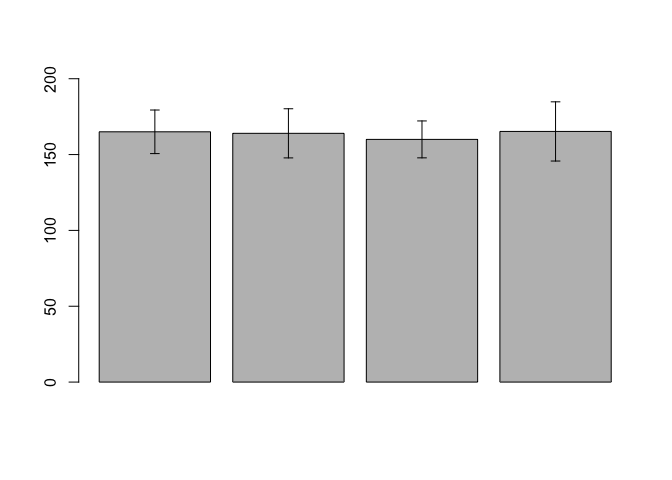
\includegraphics[width=0.9\linewidth]{_main_files/figure-latex/figName242-1} 

}

\caption{Example of a simple barplot in R}\label{fig:figName242}
\end{figure}

The graph is rather basic, but, with little exercise, we can improve it very much.

When the number of replicates is high (e.g., \textgreater{} 15), we can jointly use the 25\textsuperscript{th}, 50\textsuperscript{th} (median) and 75\textsuperscript{th} percentiles to draw the so-called \emph{boxplot} (Box-Whisker plot; Figure \ref{fig:figName241}). I will describe it by using an example: let's assume we have made an experiment with three treatments (A, B and C) and 20 replicates. We can use the code below to draw a boxplot.

\begin{Shaded}
\begin{Highlighting}[]
\FunctionTok{rm}\NormalTok{(}\AttributeTok{list =} \FunctionTok{ls}\NormalTok{())}
\NormalTok{A }\OtherTok{\textless{}{-}} \FunctionTok{c}\NormalTok{(}\DecValTok{2}\NormalTok{, }\DecValTok{31}\NormalTok{, }\DecValTok{12}\NormalTok{, }\DecValTok{12}\NormalTok{, }\DecValTok{17}\NormalTok{, }\DecValTok{13}\NormalTok{, }\DecValTok{0}\NormalTok{, }\DecValTok{5}\NormalTok{, }\DecValTok{13}\NormalTok{, }\DecValTok{10}\NormalTok{,}
       \DecValTok{14}\NormalTok{, }\DecValTok{11}\NormalTok{, }\DecValTok{6}\NormalTok{, }\DecValTok{18}\NormalTok{, }\DecValTok{6}\NormalTok{, }\DecValTok{17}\NormalTok{,  }\DecValTok{6}\NormalTok{, }\DecValTok{5}\NormalTok{, }\DecValTok{4}\NormalTok{, }\DecValTok{5}\NormalTok{)}
\NormalTok{B }\OtherTok{\textless{}{-}} \FunctionTok{c}\NormalTok{(}\DecValTok{8}\NormalTok{, }\DecValTok{8}\NormalTok{, }\DecValTok{5}\NormalTok{, }\DecValTok{3}\NormalTok{, }\DecValTok{6}\NormalTok{, }\DecValTok{18}\NormalTok{, }\DecValTok{13}\NormalTok{, }\DecValTok{20}\NormalTok{, }\DecValTok{19}\NormalTok{, }\DecValTok{3}\NormalTok{,}
       \DecValTok{11}\NormalTok{, }\DecValTok{7}\NormalTok{, }\DecValTok{8}\NormalTok{, }\DecValTok{12}\NormalTok{, }\DecValTok{6}\NormalTok{, }\DecValTok{17}\NormalTok{, }\DecValTok{6}\NormalTok{, }\DecValTok{7}\NormalTok{,  }\DecValTok{22}\NormalTok{, }\DecValTok{18}\NormalTok{)}
\NormalTok{C }\OtherTok{\textless{}{-}} \FunctionTok{c}\NormalTok{(}\DecValTok{12}\NormalTok{, }\DecValTok{12}\NormalTok{, }\DecValTok{9}\NormalTok{, }\DecValTok{7}\NormalTok{, }\DecValTok{10}\NormalTok{, }\DecValTok{22}\NormalTok{, }\DecValTok{17}\NormalTok{, }\DecValTok{24}\NormalTok{, }\DecValTok{23}\NormalTok{, }\DecValTok{7}\NormalTok{,}
       \DecValTok{15}\NormalTok{, }\DecValTok{11}\NormalTok{, }\DecValTok{12}\NormalTok{, }\DecValTok{16}\NormalTok{, }\DecValTok{10}\NormalTok{, }\DecValTok{21}\NormalTok{, }\DecValTok{10}\NormalTok{, }\DecValTok{11}\NormalTok{, }\DecValTok{26}\NormalTok{, }\DecValTok{22}\NormalTok{)}
\NormalTok{series }\OtherTok{\textless{}{-}} \FunctionTok{rep}\NormalTok{(}\FunctionTok{c}\NormalTok{(}\StringTok{"A"}\NormalTok{, }\StringTok{"B"}\NormalTok{, }\StringTok{"C"}\NormalTok{), }\AttributeTok{each =} \DecValTok{20}\NormalTok{)}
\NormalTok{values }\OtherTok{\textless{}{-}} \FunctionTok{c}\NormalTok{(A, B, C)}
\FunctionTok{boxplot}\NormalTok{(values }\SpecialCharTok{\textasciitilde{}}\NormalTok{ series)}
\end{Highlighting}
\end{Shaded}

\begin{figure}

{\centering 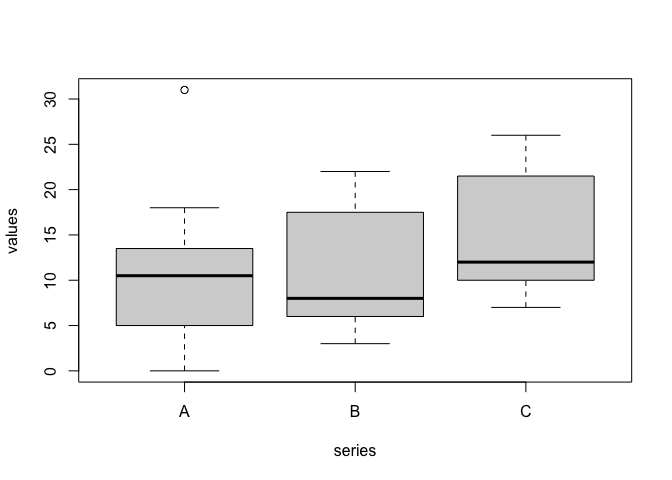
\includegraphics[width=0.9\linewidth]{_main_files/figure-latex/figName241-1} 

}

\caption{A boxplot in R}\label{fig:figName241}
\end{figure}

In this boxplot, each group is represented by a box, where the uppermost side is the 75\textsuperscript{th} percentile, the lowermost side is the 25\textsuperscript{th} percentile, while a line is drawn to indicate the median (50\textsuperscript{th} percentile). Two vertical arrows (whiskers) start from the 25\^{}th and 75\^{}th percentile and reach the maximum and minimum values for each group. In the case of treatment A, the maximum value is 31, which is 20.5 units above the median. As this difference is higher than 1.5 times the difference from the median and the 75\textsuperscript{th} percentile, this value is excluded, it is regarded as an outlier and it is represented by an empty circle.

For the case when we have a pair of quantitative variables, we can draw a \textbf{scatterplot}, by using the two variables as the co-ordinates. The simplest R plotting function is \texttt{plot()} and an example of its usage is given in Figure \ref{fig:figName244}), with reference to the correlation data at 3.1.5.

\begin{Shaded}
\begin{Highlighting}[]
\FunctionTok{plot}\NormalTok{(A }\SpecialCharTok{\textasciitilde{}}\NormalTok{ B, }\AttributeTok{xlab =} \StringTok{"b"}\NormalTok{, }\AttributeTok{ylab =} \StringTok{"a"}\NormalTok{,}
     \AttributeTok{pch =} \DecValTok{21}\NormalTok{, }\AttributeTok{col =} \StringTok{"blue"}\NormalTok{, }\AttributeTok{cex =} \DecValTok{2}\NormalTok{, }\AttributeTok{bg =} \StringTok{"blue"}\NormalTok{)}
\end{Highlighting}
\end{Shaded}

\begin{figure}

{\centering 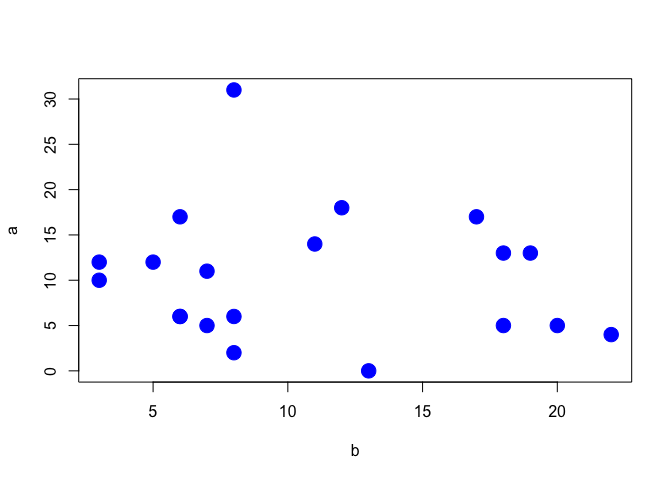
\includegraphics[width=0.9\linewidth]{_main_files/figure-latex/figName244-1} 

}

\caption{Scatterplot showing the correlation between two variables}\label{fig:figName244}
\end{figure}

A distribution of frequency can also be represented by using a \textbf{pie chart}, as shown in Figure \ref{fig:figName243}), for the `gear' variable in the `mtcars' dataset.

\begin{Shaded}
\begin{Highlighting}[]
\FunctionTok{pie}\NormalTok{(}\FunctionTok{table}\NormalTok{(mtcars}\SpecialCharTok{$}\NormalTok{gear))}
\end{Highlighting}
\end{Shaded}

\begin{figure}

{\centering 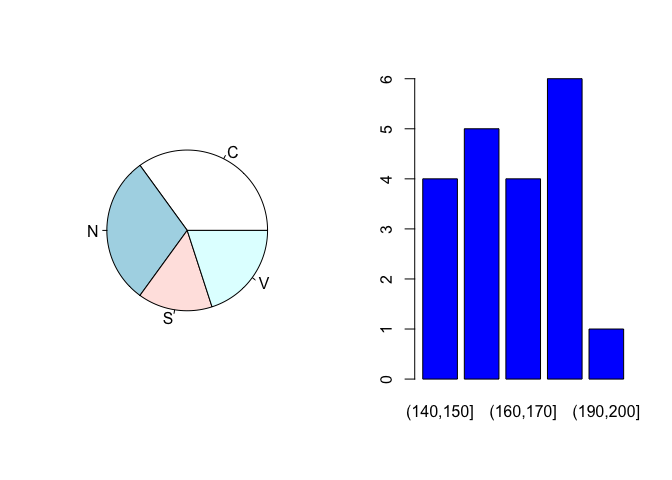
\includegraphics[width=0.65\linewidth]{_main_files/figure-latex/figName243-1} 

}

\caption{Representation of a distribution of frequencies by using a pie chart}\label{fig:figName243}
\end{figure}

\begin{center}\rule{0.5\linewidth}{0.5pt}\end{center}

\hypertarget{further-reading}{%
\section{Further reading}\label{further-reading}}

\begin{enumerate}
\def\labelenumi{\arabic{enumi}.}
\tightlist
\item
  Holcomb Z.C. (2017). Fundamentals of descriptive statistics. Routledge (Taylor and Francis Group), USA
\end{enumerate}

\hypertarget{modeling-the-experimental-data}{%
\chapter{Modeling the experimental data}\label{modeling-the-experimental-data}}

In the previous chapter we have seen that we can use simple stats to describe, summarise and present our experimental data, which is usually the very first step of data analyses. However, we are more ambitious: we want to model our experimental data. Perhaps this term sounds unfamiliar to some of you and, therefore, we should better start by defining the terms `model' and `modeling.'

A mathematical model is the description of a system using the mathematical language and the process of developing a model is named mathematical modeling. In practice, we want to write an equation where our experimental observations are obtained as the result of a set of predictors and operators.

Writing mathematical models for natural processes has been one of the greatest scientific challenges, since the 19th century and it may be appropriately introduced by using a very famous quote from Pierre-Simon Laplace (1749-1827): ``\emph{We ought to regard the present state of the universe as the effect of its antecedent state and as the cause of the state that is to follow. An intelligence knowing all the forces acting in nature at a given instant, as well as the momentary positions of all things in the universe, would be able to comprehend in one single formula the motions of the largest bodies as well as the lightest atoms in the world, provided that its intellect were sufficiently powerful to subject all data to analysis; to it nothing would be uncertain, the future as well as the past would be present to its eyes. The perfection that the human mind has been able to give to astronomy affords but a feeble outline of such an intelligence.}''

Working in biology and agriculture, we need to recognise that we are very far away from Laplace's ambition; indeed, the systems which we work with are very complex and they are under the influence of a high number of external forces in strong interaction with one another. The truth is that we know too little to be able to predict the future state of the agricultural systems; think about the yield of a certain wheat genotype: in spite of our research effort, we are not yet able to forecast future yield levels, because, e.g., we are not yet able to forecast the weather for future seasons.

In this book, we will not try to write models to predict future outcomes for very complex systems; we will only write simple models to describe the responses obtained from controlled experiments, where the number of external forces has been reduced to a minimum level. You might say that modeling the past is rather a humble aim, but we argue that this is challenging enough\ldots{}

One first problem we have to solve is that our experimental observations are always affected by:

\begin{enumerate}
\def\labelenumi{\arabic{enumi}.}
\tightlist
\item
  deterministic effects, working under a cause-effect relationship;
\item
  stochastic effects, of purely random nature, which induce more or less visible differences among the replicates of the same measurement.
\end{enumerate}

Clearly, every good descriptive model should contain two components, one for each of the above mentioned groups of effects. Models containing a random component are usually named `statistical models,' as opposed to `mathematical models,' which tend to disregard the stochastic effects.

\hypertarget{deterministic-models}{%
\section{Deterministic models}\label{deterministic-models}}

Based on the Galileian scientific approach, our hypothesis is that all biological phoenomena are based on an underlying mechanism, which we describe by using a deterministic (cause-effect) model, where:

\[ Y_E = f(X, \theta) \]

In words, the expected outcome \(Y_E\) is obtained as a result of the \emph{stimulus} \(X\), according to the function \(f\), based on a number of parameters \(\theta\); this simple cause-effect model, with loose language, can be called a dose-response model.

Let's look at model components in more detail. In a previous chapter we have seen that the expected response \(Y_E\) can take several forms, i.e.~it can be either a quantity, or a count, or a ratio or a quality. The expected response can be represented by one single variable (univariate response) or by several variables (multivariate response) and, in this book, we will only consider the simplest situation (univariate response).

The experimental stimulus (\(X\)) is represented by one or more quantitative/categorical variables, usually called predictors, while the response function \(f\) is a linear/non-linear equation, that is usually selected according to the biological mechanism of the process under investigation. Very often, equations are selected in a purely empirical fashion: we look at the data and select a suitable curve shape.

Every equation is based on a number of parameters, which are generally indicated by using Greek or Latin letters. In this book we will use \(\theta\) to refer to the whole set of parameters in a deterministic model.

Let's see a few examples of deterministic models. The simplest model is the so-called \emph{model of the mean}, that is expressed as:

\[ Y = \mu \]

According to this simple model, the observations should be equal to some pre-determined value (\(\mu\)); \(f\) is the identity function with only one parameter (\(\theta = \mu\)) and no predictors. In this case, we do not need predictors, as the experiment is not comparative, but, simply, mensurative. For a comparative experiment, where we have two or more stimula, the previous model can be expanded as follows:

\vspace{12pt}

\[
Y = \left\{ {\begin{array}{ll}
\mu_A \quad \textrm{if} \,\, X = A \\
\mu_B \quad \textrm{if} \,\, X = B
\end{array}} \right.
\]

This is a simple example of the so-called \emph{ANOVA models}, where the response depends on the stimulus and subjects treated with A return a response equal to \(\mu_A\), while subjects treated with B return a response equal to \(\mu_B\). The response is quantitative, but the predictor represents the experimental treatments and it is described by using a categorical variable, with two levels. We can make it more general by writing:

\[Y = \mu_j\]

where \(j\) represents the experimental treatment.

Another important example is the \emph{simple linear regression model}, where the relationship between the predictor and the response is described by using a `straight line':

\[ Y = \beta_0 + \beta_1 \times X \]

In this case, both \(Y\) and \(X\) are quantitative variables and we have two parameters, i.e.~\(\theta = [\beta_0, \beta_1]\).

We can also describe curvilinear relationships by using other models, such as a second order polynomial (three parameters):

\[ Y = \beta_0 + \beta_1 \, X + \beta_2 \, X^2\]

or the exponential function (two parameters, \(e\) is the Nepero operator):

\[ Y = \beta_0 \, e^{\beta_1 X} \]

We will see some more examples of curvilinear functions near to the end of this book.

Whatever it is, the function \(f\) needs to be fully specified, i.e.~we need to give a value to all unknown parameters. Consider the following situation: we have a well that is polluted by herbicide residues to a concentration of 120 mg/L. If we analyse a water sample from that well, we should expect that the concentration is \(Y_E = 120\) (model of the mean). Likewise, if we have two genotypes (A and B), their yield in a certain pedo-climatic condition could be described by an ANOVA model, where we specify that, e.g.,

\[
Y = \left\{ {\begin{array}{ll}
27 \quad \textrm{if} \,\, X = A \\
32 \quad \textrm{if} \,\, X = B
\end{array}} \right.
\]

As a third example of a fully specified model, we could assume that the yield response of wheat in some specific environmental conditions is related to N fertilisation, by way of a linear function \(Y = \beta_0 + \beta_1 \times X\), where \(\beta_0 = 20\) e \(\beta_1 = 0.3\) (i.e.~\(\theta = [20, 0.3]\)). In this case, the model is \(Y = 20 + 0.3 \times X\) and we can use it to predict the yield response to, e.g., 0, 30, 60, 90, 120 and 150 kg N ha\textsuperscript{-1}, as shown below:

\begin{Shaded}
\begin{Highlighting}[]
\NormalTok{X }\OtherTok{\textless{}{-}} \FunctionTok{c}\NormalTok{(}\DecValTok{0}\NormalTok{, }\DecValTok{30}\NormalTok{, }\DecValTok{60}\NormalTok{, }\DecValTok{90}\NormalTok{, }\DecValTok{120}\NormalTok{, }\DecValTok{150}\NormalTok{)}
\NormalTok{Ye }\OtherTok{\textless{}{-}} \DecValTok{20} \SpecialCharTok{+} \FloatTok{0.3} \SpecialCharTok{*}\NormalTok{ X}
\NormalTok{Ye}
\DocumentationTok{\#\# [1] 20 29 38 47 56 65}
\end{Highlighting}
\end{Shaded}

You may argue that this latter example is not realistic, as the relationship between N fertilisation and yield can never be linear, but, presumably, asymptotic. You are right, but that does not matter at this moment; our point is that \textbf{we can postulate the existence of an underlying, unknown mechanism that produces our experimental outcomes, by following a fully specified deterministic cause-effect model}.

\hypertarget{stochastic-models}{%
\section{Stochastic models}\label{stochastic-models}}

In practice, reality is more complex than our expectations and, due to experimental errors, we do never observe the expected outcome. Therefore, modelling the observations requires that we introduce the effect of unknown entities. It would seem a nonsense\ldots{} how can we predict the effects of something we do not even know?

Let's go back to the example of the polluted well, where we would expect that the concentration is \(Y_E = 120\) mg/L. It is very easy to imagine that the above mechanism is overly simplistic, due to the fact that our chemical instrument is not free from measurement errors. Indeed, if we measure the concentration of several water samples from the same well, we will not always obtain exactly 120 mg/L, but we will obtain a set of values more or less different from each other. We could model this by writing that the observed values \(Y_O \neq Y_E\) is:

\[Y_O = 120 + \varepsilon\]

where \(\varepsilon\) is an individual random component that brings our measure away from the expected value. Do we have any hints on how to determine \(\varepsilon\)? If we had enough knowledge to understand the exact cause for the effect \(\varepsilon\) we could incorporate it into the deterministic model. As we do not have enough knowledge at the moment, we need to find another way to model this stochastic component.

Indeed, although we cannot precisely determine \(\varepsilon\) for each single water sample, we can make some reasonable assumptions. If the expected value is 120 mg/L (this is indeed the underlying mechanism we postulate), we should expect that it is likely to find a cooncentration of 119 or 121 mg/L (\(\varepsilon = \pm 1\)), less likely to find a concentration of 100 or 140 mg/L (\(\varepsilon = \pm 20\)), very unlikely to find a concentration of 80 or 160 mg/L (\(\varepsilon = \pm 40\)). Consequently, it should be possible to assign a value of probability to each possible \(\varepsilon\) value (and thus to each possible \(Y_O\) value), by using some sort of probability function.

\hypertarget{probability-functions}{%
\subsection{Probability functions}\label{probability-functions}}

How do we assign the probability to a stochastic experimental outcome? This is rather easy when the outcome \(Y_O\) is categorical and can only take one of a finite list of possible values \(y\). For example, let's consider an experiment where we sample a wheat plant from a population and count the number of lateral tillers, so that \(Y_O\) can only take an integer value from, e.g., 0 to 3. The probability of finding a plant with, e.g., one lateral tiller (\(Y_O\) = 1) is equal to the number of subjects with one lateral tiller divided by the total number of subjects within the population (frequentist definition of probability). If the population consists of 20 plants and, among those, 4 plants have no lateral tillers, 6 plants have one tiller, 8 plants have 2 tillers and 2 plants have three tillers, the probabilities for all the possible outcomes are:

\[P(Y_O = y) = \left\{ \begin{array}{l}
 4/20 = 0.2 \,\,\,\,\,\,\textrm{if}\,\,\,\,\,\, y = 0 \\ 
 6/20 = 0.3 \,\,\,\,\,\,\textrm{if}\,\,\,\,\,\, y = 1 \\ 
 8/20 = 0.4\,\,\,\,\,\, \textrm{if}\,\,\,\,\,\, y = 2 \\ 
 2/20 = 0.1 \,\,\,\,\,\,\textrm{if}\,\,\,\,\,\, y = 3 \\ 
 \end{array} \right.\]

In the above equation, P is a \textbf{Probability Mass Function} (PMF) or, more simply a \textbf{Probability Function} and it takes the form of a distribution of relative frequencies. It does not help us to predict the outcome of our sampling experiment, but it gives us an idea of what it is more likely to happen.

What are the main characteristics of a probability function? Two rules are fundamental:

\begin{enumerate}
\def\labelenumi{\arabic{enumi}.}
\tightlist
\item
  \(P(Y_O = y)\) must always be positive, for every possible \(y\) value;
\item
  the probabilities for all possible events \(y\) must sum up to one, i.e.~\(\sum{P \left(Y_O = y \right)} = 1\)
\end{enumerate}

With ordinal classes (as in our example), we can also define the \textbf{Cumulative Distribution Function} (CDFs), as the sum of the probabilities of one event with all the `previous' ones, i.e.:

\[P(Y_O \le y) = \sum_{y_k \le y}{P(Y_O = y_k)}\]

For our wheat tillers example, we have:

\[P(Y_O \le y) = \left\{ \begin{array}{l}
 0.2\,\,\,\,\,\,\textrm{if}\,\,\,\,\,\, y \leq 0 \\ 
 0.5\,\,\,\,\,\,\textrm{if}\,\,\,\,\,\, y \leq 1 \\ 
 0.9\,\,\,\,\,\,\textrm{if}\,\,\,\,\,\, y \leq 2 \\ 
 1.0\,\,\,\,\,\,\textrm{if}\,\,\,\,\,\, y \leq 3 \\ 
 \end{array} \right.\]

For these PDFs, using the information given in Chapter 3, we can calculate descriptive statistics, such as the mean (expected value) and the variance:

\[\mu  = \sum{\left[ y_k \cdot P(Y_O = y_k ) \right]}\]

\[\sigma ^2  = \sum{ \left[ {\left( {y_k  - \mu } \right)^2 \cdot P(Y_O = y_k)} \right]}\]

In our example, it is:

\begin{Shaded}
\begin{Highlighting}[]
\NormalTok{mu }\OtherTok{\textless{}{-}} \DecValTok{0} \SpecialCharTok{*} \FloatTok{0.2} \SpecialCharTok{+} \DecValTok{1} \SpecialCharTok{*} \FloatTok{0.3} \SpecialCharTok{+} \DecValTok{2} \SpecialCharTok{*} \FloatTok{0.4} \SpecialCharTok{+} \DecValTok{3} \SpecialCharTok{*} \FloatTok{0.1}
\NormalTok{mu}
\DocumentationTok{\#\# [1] 1.4}
\end{Highlighting}
\end{Shaded}

and:

\begin{Shaded}
\begin{Highlighting}[]
\NormalTok{sigma2 }\OtherTok{\textless{}{-}}\NormalTok{ (}\DecValTok{0} \SpecialCharTok{{-}}\NormalTok{ mu)}\SpecialCharTok{\^{}}\DecValTok{2} \SpecialCharTok{*} \FloatTok{0.2} \SpecialCharTok{+}\NormalTok{ (}\DecValTok{1} \SpecialCharTok{{-}}\NormalTok{ mu)}\SpecialCharTok{\^{}}\DecValTok{2} \SpecialCharTok{*} \FloatTok{0.3} \SpecialCharTok{+}\NormalTok{ (}\DecValTok{2} \SpecialCharTok{{-}}\NormalTok{ mu)}\SpecialCharTok{\^{}}\DecValTok{2} \SpecialCharTok{*} 
  \FloatTok{0.3} \SpecialCharTok{+}\NormalTok{ (}\DecValTok{3} \SpecialCharTok{{-}}\NormalTok{ mu)}\SpecialCharTok{\^{}}\DecValTok{2} \SpecialCharTok{*} \FloatTok{0.2}
\NormalTok{sigma2  }
\DocumentationTok{\#\# [1] 1.06}
\end{Highlighting}
\end{Shaded}

On average, our plants have 1.4 lateral tillers, with a variance of 1.06.

\hypertarget{density-functions}{%
\subsection{Density functions}\label{density-functions}}

For quantitative variables, the outcome may take any value within a certain interval. Is it sensible to ask what probability we have to measure a concentration value that is exactly, e.g., 120 mg/L (not 120.0000001 or 119.99999 mg/L)? We do understand that such a probability is infinitesimal. In general, we cannot calculate the probability of a `point-event' for continuous variables.

We can think of dividing the concentration scale into a finite number of intervals, e.g.~\textless{} 100 mg/L, from 100 to 110 mg/L, from 110 to 120 mg/L and so on (binning; we spoke about this in Chapter 3), so that all individuals in the population can be assigned to one and only one interval. It is intuitively clear that we can always calculate the probability of one interval as the ratio between the number of individuals in that interval and the total number of individuals in the population. However, a new problem arises when we try to define a probability function: how should we select the width of intervals?

A possible solution is that we calculate the so-called \textbf{probability density}, i.e.~the ratio of the probability mass in one interval to the interval width. For example, if we have a probability mass of 0.3 in the interval between 110 to 130 \(mg/L\), the probability density is:

\[D([110, 130]) = \frac{P([110,130])}{20} = \frac{0.3}{20}\]

Why do we talk about `density?' Because this is, indeed, a probability mass per unit interval (do you remember? the usual density is a mass per unit volume).

Now we can wonder: what happens with the density, when the interval becomes smaller and smaller? This is shown in Figure \ref{fig:figName50b}; we can see that when the interval width tends to 0, the density tends to assume a finite value, according to the red function in Figure \ref{fig:figName50b} (bottom right).

\begin{figure}

{\centering 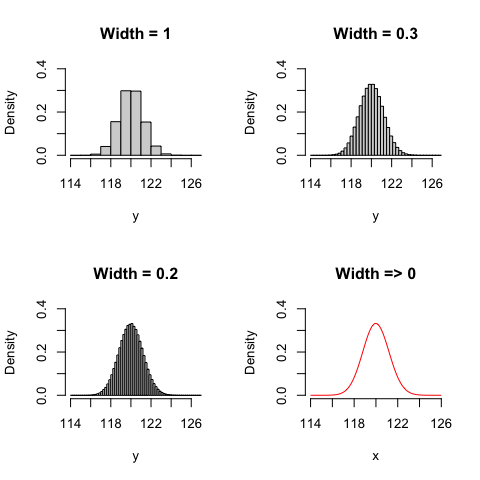
\includegraphics{_main_files/figure-latex/figName50b-1} 

}

\caption{Probability density function, depending on the width of the interval}\label{fig:figName50b}
\end{figure}

In the end, dealing with a continuous variable, we cannot calculate the probability of a `point-event,' but we can calculate its density. Therefore, instead of defining a probability function, we can define a \textbf{Probability Density Function} (PDF), depicting the density of all possible events.

The most common PDF is the Gaussian PDF, that is also known as the \textbf{normal curve}; it is represented in the bottom right panel of Figure \ref{fig:figName50b} and it is introduced in the following section.

\hypertarget{the-gaussian-pdf-and-cdf}{%
\subsection{The Gaussian PDF and CDF}\label{the-gaussian-pdf-and-cdf}}

The Gaussian PDF is defined as:

\[\phi(y) = \frac{1}{{\sigma \sqrt {2\pi } }}\exp \left[{\frac{\left( {y - \mu } \right)^2 }{2\sigma ^2 }} \right]\]

where \(\phi(y)\) is the probability density that the observed outcome assume the value \(y\), while \(\mu\) and \(\sigma\) are the parameters. The gassian PDF is continuous and it is defined from \(-\infty\) to \(\infty\).

The density in itself is not very much useful for our task; how can we use the density to calculate the probability for an outcome \(Y_O\) that is comprised between any two values \(y_1\) and \(y_2\)?. Let's recall that the density is the probability mass per unit interval width; therefore, if we multiply the density by the interval width, we get the probability for that interval. We can imagine that the area under the gaussian curve in Figure \ref{fig:figName50b} (bottom right) is composed by a dense comb of tiny rectangles with very small widths; the area of each rectangle is obtained as the product of a density (height) by the interval width and, therefore, it represents a probability. Consequently, if we take any two values \(y_1\) and \(y_2\), the probability of the corresponding interval can be obtained as the sum of the areas of all the tiny rectangles between \(y_1\) and \(y_2\). In other words, the probability of an interval can be obtained as the Area Under the Curve (AUC). You may recall from high school that the AUC is, indeed, the integral of the gaussian curve from \(y_1\) and \(y_2\):

\[P(y_1 \le Y_O < y_2) = \int\limits_{ y_1 }^{y_2} {\phi(y)} dy\]

Analogously, we can obtain the corresponding CDF, by:

\[P(Y_O \le y) = \int\limits_{ -\infty }^{y} {f(y)} dy\]

You may have noted that this is totally the same as the PDF for a discrete variable, although the summation has become an integral.

If the PDF is the defined as the function \(\phi(y)\), the mean and variance for \(\phi\) can also be calculated as shown above for the probability functions, by replacing summations with integrals:

\[\begin{array}{l}
\mu  = \int\limits_{ - \infty }^{ + \infty } {y f(y)} dy \\ 
\sigma ^2  = \int\limits_{ - \infty }^{ + \infty } {\left( {y - \mu } \right)^2 f(y)} dy
\end{array}\]

I will not go into much mathematical detail, but it is useful to note that, with a Gaussian CDF:

\begin{enumerate}
\def\labelenumi{\arabic{enumi}.}
\tightlist
\item
  the curve shape depends only on the values of \(\mu\) and \(\sigma\) (Figure \ref{fig:figName51} ). It means that if we start from the premise that a population of measures is Gaussian distributed (normally distributed), knowing the mean and the standard deviation is enough to characterise the whole population. Such a premise is usually called \textbf{parametric assumption}.
\item
  The curve has two asymptotes and the limits when \(y\) goes to \(\pm \infty\) are 0. It is implied that every \(y\) values is a possible outcome for our experiment, although the probabilities of very small and very high values are negligible.
\item
  The integral of the Gauss curve from \(- \infty\) to \(+ \infty\) is 1, as this is the sum of the probability densities for all possible outcomes.
\item
  The area under the Gaussian curve between two points (integral) represents the probability of obtaining values within the corresponding interval. For example, Figure \ref{fig:figName52} shows that 80\% of the individuals lie within the interval from \(-\infty\) to, roughly, 1;
\item
  The curve is symmetrical around the mode, that is equal to the median and the mean. That is, the probability density of values above the mean and below the mean is equal.
\item
  We can calculate that, for given \(\mu\) and \(\sigma\), the probability density of individuals within the interval from \(\mu\) to \(\mu + \sigma\) is 15.87\% and it is equal to the probability density of the individuals within the interval from \(\mu - \sigma\) to \(\mu\).
\end{enumerate}

\begin{figure}

{\centering 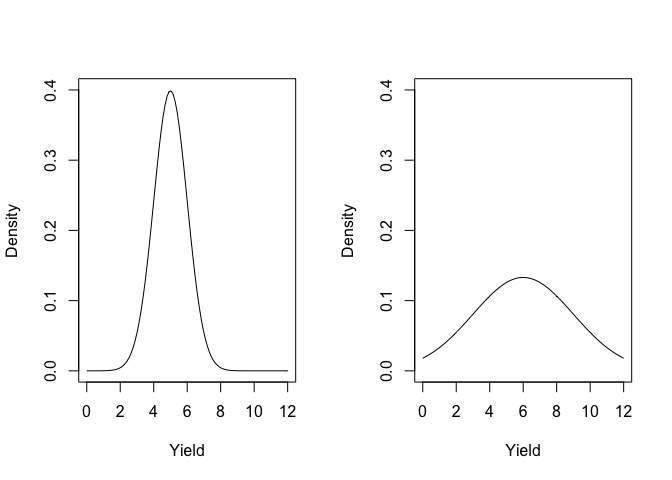
\includegraphics[width=0.9\linewidth]{_main_files/figure-latex/figName51-1} 

}

\caption{The shape of the gaussian function, depending on the mean and standard deviation (left: mean = 5 and SD = 1; right: mean = 6 and SD = 3)}\label{fig:figName51}
\end{figure}

\begin{figure}

{\centering 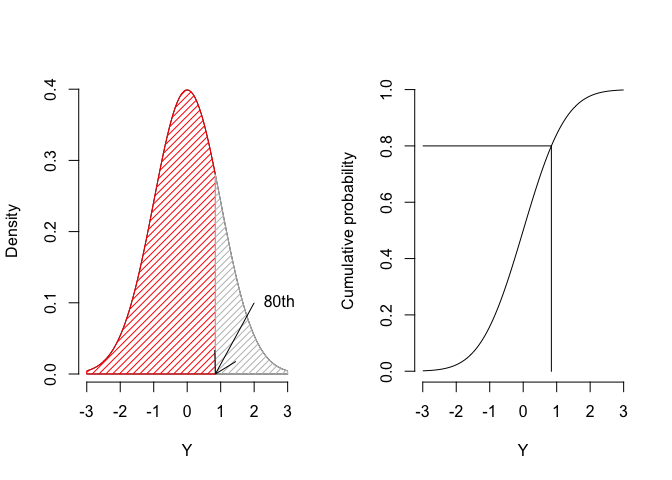
\includegraphics[width=0.9\linewidth]{_main_files/figure-latex/figName52-1} 

}

\caption{Getting the 80th percentile as the area under the PDF curve (left) and from the CDF (right)}\label{fig:figName52}
\end{figure}

\hypertarget{a-model-with-two-components}{%
\section{A model with two components}\label{a-model-with-two-components}}

Let's go back to our example with the polluted well. We said that, on average, the measure should be 120 mg/L, but we also said that each individual measure has its own random component \(\epsilon\), so that \(Y_O = 120 + \varepsilon\). The stochastic element cannot be predicted, but we can use the Gaussian to calculate the probability of any outcome \(Y_O\).

Now we are ready to write a two-components model for our herbicide concentrations, in relation to each possible water sample \(i\):

\[y_i = \mu + \varepsilon_i\]

where the stochastic element \(\varepsilon\) is:

\[ \varepsilon \sim \textrm{Norm}(0, \sigma) \]

The above equation means that the stochastic element is gaussian distributed with mean equal to 0 and standard deviation equal to \(\sigma\). Another equivalent form is:

\[Y_i \sim \textrm{Norm}(\mu, \sigma)\]

which says that the concentration is gaussian distributed with mean \(\mu = 120\) (the deterministic part) and standard deviation equal to \(\sigma\).

In our example, if we assume that \(\sigma = 12\) (the stochastic part), we can give the best possible description of all concentration values for all possible water samples from our polluted well. For example, we can answer the following questions:

\begin{enumerate}
\def\labelenumi{\arabic{enumi}.}
\tightlist
\item
  What is the most likely concentration value?
\item
  What is the probability density of finding a water sample with a concentration of 100 mg/L?
\item
  What is the probability of finding a water sample with a concentration lower than 100 mg/L?
\item
  What is the probability of finding a water sample with a concentration higher than 140 mg/L?
\item
  What is the probability of finding a water sample with a concentration within the interval from 100 to 140 mg/L?
\item
  What is the 80th percentile, i.e.~the concentration which is higher than 80\% of all possible water samples?
\item
  What are the two values, symmetrical around the mean, which contain the concentrations of 95\% of all possible water samples?
\end{enumerate}

Question 1 is obvious. In order to answer all the above questions from 2 on, we need to use the available R function for gaussian distribution. For every distribution, we have a PDF (the prefix is always `d'), a CDF (the prefix is `p') and a quantile function (the prefix is `q'), that is the inverse CDF, giving the value corresponding to a given percentile. For the Gaussian function, the name is `norm,' so that we have the R functions \texttt{dnorm()}, \texttt{pnorm()} and \texttt{qnorm()}. The use of these functions is straightforward:

\begin{Shaded}
\begin{Highlighting}[]
\CommentTok{\# Question 2}
\FunctionTok{dnorm}\NormalTok{(}\DecValTok{100}\NormalTok{, }\AttributeTok{mean =} \DecValTok{120}\NormalTok{, }\AttributeTok{sd =} \DecValTok{12}\NormalTok{)}
\DocumentationTok{\#\# [1] 0.008289762}
\end{Highlighting}
\end{Shaded}

\begin{Shaded}
\begin{Highlighting}[]
\CommentTok{\# Question 3}
\FunctionTok{pnorm}\NormalTok{(}\DecValTok{100}\NormalTok{, }\AttributeTok{mean =} \DecValTok{120}\NormalTok{, }\AttributeTok{sd =} \DecValTok{12}\NormalTok{)}
\DocumentationTok{\#\# [1] 0.04779035}
\end{Highlighting}
\end{Shaded}

For the 4th question we should consider that cumulative probabilities are given for the lower curve tail, while we were asked to determine the higher tail. Therefore, we have two possible solutions, as shown below:

\begin{Shaded}
\begin{Highlighting}[]
\CommentTok{\# Question 4}
\DecValTok{1} \SpecialCharTok{{-}} \FunctionTok{pnorm}\NormalTok{(}\DecValTok{140}\NormalTok{, }\AttributeTok{mean =} \DecValTok{120}\NormalTok{, }\AttributeTok{sd =} \DecValTok{12}\NormalTok{)}
\DocumentationTok{\#\# [1] 0.04779035}
\FunctionTok{pnorm}\NormalTok{(}\DecValTok{140}\NormalTok{, }\AttributeTok{mean =} \DecValTok{120}\NormalTok{, }\AttributeTok{sd =} \DecValTok{12}\NormalTok{, }\AttributeTok{lower.tail =}\NormalTok{ F)}
\DocumentationTok{\#\# [1] 0.04779035}
\end{Highlighting}
\end{Shaded}

\begin{Shaded}
\begin{Highlighting}[]
\CommentTok{\# Question 5}
\FunctionTok{pnorm}\NormalTok{(}\DecValTok{140}\NormalTok{, }\AttributeTok{mean =} \DecValTok{120}\NormalTok{, }\AttributeTok{sd =} \DecValTok{12}\NormalTok{) }\SpecialCharTok{{-}} \FunctionTok{pnorm}\NormalTok{(}\DecValTok{100}\NormalTok{, }\AttributeTok{mean =} \DecValTok{120}\NormalTok{, }\AttributeTok{sd =} \DecValTok{12}\NormalTok{)}
\DocumentationTok{\#\# [1] 0.9044193}
\end{Highlighting}
\end{Shaded}

In order to calculate the percentiles we use the \texttt{qnorm()} function:

\begin{Shaded}
\begin{Highlighting}[]
\CommentTok{\# Question 6}
\FunctionTok{qnorm}\NormalTok{(}\FloatTok{0.8}\NormalTok{, }\AttributeTok{mean =} \DecValTok{120}\NormalTok{, }\AttributeTok{sd =} \DecValTok{12}\NormalTok{)}
\DocumentationTok{\#\# [1] 130.0995}
\end{Highlighting}
\end{Shaded}

\begin{Shaded}
\begin{Highlighting}[]
\CommentTok{\# Question 7}
\FunctionTok{qnorm}\NormalTok{(}\FloatTok{0.025}\NormalTok{, }\AttributeTok{mean =} \DecValTok{120}\NormalTok{, }\AttributeTok{sd =} \DecValTok{12}\NormalTok{)}
\DocumentationTok{\#\# [1] 96.48043}
\FunctionTok{qnorm}\NormalTok{(}\FloatTok{0.975}\NormalTok{, }\AttributeTok{mean =} \DecValTok{120}\NormalTok{, }\AttributeTok{sd =} \DecValTok{12}\NormalTok{)}
\DocumentationTok{\#\# [1] 143.5196}
\end{Highlighting}
\end{Shaded}

\hypertarget{and-so-what}{%
\section{And so what?}\label{and-so-what}}

Let's summarise:

\begin{enumerate}
\def\labelenumi{\arabic{enumi}.}
\tightlist
\item
  we use deterministic cause-effect models to predict the average behavior in a population
\item
  we cannot predict the exact outcome of each single experiment, but we can calculate the probability of obtaining one of several possible outcomes by using stochastic models, in the form of PDFs
\end{enumerate}

In order to do so, we need to be able to assume what the form is for the PDF within the population (\textbf{parametric assumption}). Indeed, such a form can only be assumed, unless we know the whole population, which is impossible as long as we are making an experiment to know the population itself.

\hypertarget{monte-carlo-methods-to-simulate-an-experiment}{%
\section{Monte Carlo methods to simulate an experiment}\label{monte-carlo-methods-to-simulate-an-experiment}}

Considering the above process, the results of every experiment can be simulated by using the so-called Monte Carlo methods, which can reproduce the mechanisms of natural phenomena. These methods are based on random number generators; for example, in R, it is possible to produce random numbers from a given PDF, by using several functions prefixed by `r.' For example, the gaussian random number generator is \texttt{rnorm()}.

Let's go back to our polluted well. If we know that the concentration is exactly 120 mg/L, we can reproduce the results of an experiment where we analyse three replicated water samples, by using an instrument with 10\% coefficient of variability (that is \(\sigma = 12\)).

With R, the process is as follows:

\begin{Shaded}
\begin{Highlighting}[]
\FunctionTok{set.seed}\NormalTok{(}\DecValTok{1234}\NormalTok{)}
\NormalTok{Y\_E }\OtherTok{\textless{}{-}} \DecValTok{120}
\NormalTok{epsilon }\OtherTok{\textless{}{-}} \FunctionTok{rnorm}\NormalTok{(}\DecValTok{3}\NormalTok{, }\DecValTok{0}\NormalTok{, }\DecValTok{12}\NormalTok{)}
\NormalTok{Y\_O }\OtherTok{\textless{}{-}}\NormalTok{ Y\_E }\SpecialCharTok{+}\NormalTok{ epsilon}
\NormalTok{Y\_O}
\DocumentationTok{\#\# [1] 105.5152 123.3292 133.0133}
\end{Highlighting}
\end{Shaded}

We need to note that, at the very beginning, we set the seed to the value of `1234.' Indeed, random numbers are, by definition, random and, therefore, we should all obtain different values at each run. However, random number generators are based on an initial `seed' and, if you and I set the same seed, we can obtain the same random values, which is handy, for the sake of reproducibility. Please, also note that the first argument to the \texttt{rnorm()} function is the required number of random values.

The very same approach can be used with more complex experiments:

\begin{enumerate}
\def\labelenumi{\arabic{enumi}.}
\tightlist
\item
  simulate the expected results by using the selected deterministic model,
\item
  attached random variability to the expected outcome, by sampling from the appropriate probability density function, usually by a gaussian.
\end{enumerate}

In the box below we show how to simulate the results of an experiment where we compare the yield of wheat treated with four different nitrogen rates (0, 60, 120 e 180 kg/ha), on an experiment with four replicates (sixteen data in all).

\begin{Shaded}
\begin{Highlighting}[]
\FunctionTok{set.seed}\NormalTok{(}\DecValTok{1234}\NormalTok{)}
\NormalTok{Dose }\OtherTok{\textless{}{-}} \FunctionTok{rep}\NormalTok{(}\FunctionTok{c}\NormalTok{(}\DecValTok{0}\NormalTok{, }\DecValTok{60}\NormalTok{, }\DecValTok{120}\NormalTok{, }\DecValTok{180}\NormalTok{), }\AttributeTok{each=}\DecValTok{4}\NormalTok{) }
\NormalTok{Yield\_E }\OtherTok{\textless{}{-}} \DecValTok{25} \SpecialCharTok{+} \FloatTok{0.15} \SpecialCharTok{*}\NormalTok{ Dose}
\NormalTok{epsilon }\OtherTok{\textless{}{-}} \FunctionTok{rnorm}\NormalTok{(}\DecValTok{16}\NormalTok{, }\DecValTok{0}\NormalTok{, }\FloatTok{2.5}\NormalTok{)}
\NormalTok{Yield }\OtherTok{\textless{}{-}}\NormalTok{ Yield\_E }\SpecialCharTok{+}\NormalTok{ epsilon}
\NormalTok{dataset }\OtherTok{\textless{}{-}} \FunctionTok{data.frame}\NormalTok{(Dose, Yield)}
\NormalTok{dataset}
\DocumentationTok{\#\#    Dose    Yield}
\DocumentationTok{\#\# 1     0 21.98234}
\DocumentationTok{\#\# 2     0 25.69357}
\DocumentationTok{\#\# 3     0 27.71110}
\DocumentationTok{\#\# 4     0 19.13576}
\DocumentationTok{\#\# 5    60 35.07281}
\DocumentationTok{\#\# 6    60 35.26514}
\DocumentationTok{\#\# 7    60 32.56315}
\DocumentationTok{\#\# 8    60 32.63342}
\DocumentationTok{\#\# 9   120 41.58887}
\DocumentationTok{\#\# 10  120 40.77491}
\DocumentationTok{\#\# 11  120 41.80702}
\DocumentationTok{\#\# 12  120 40.50403}
\DocumentationTok{\#\# 13  180 50.05937}
\DocumentationTok{\#\# 14  180 52.16115}
\DocumentationTok{\#\# 15  180 54.39874}
\DocumentationTok{\#\# 16  180 51.72429}
\end{Highlighting}
\end{Shaded}

\hypertarget{data-analysis-and-model-fitting}{%
\section{Data analysis and model fitting}\label{data-analysis-and-model-fitting}}

So far, we have shown how we can model the outcome of scientific experiments. In practise, we have assumed that we knew the function \(f\), the parameters \(\theta\), the predictors \(X\) the PDF type and \(\sigma\). With such knowledge, we have produced the response \(y_i\). In an experimental setting the situation is the reverse: we know the predictors \(X\), the measured response \(y_i\) and we can assume a certain form for \(f\) and for the PDF, but we do not know \(\theta\) and \(\sigma\).

Therefore, we use the observed data to estimate \(\theta\) and \(\sigma\). We see that we are totally following the Galileian process, by posing our initial hypothesis in the form of a mathematical model. This process is named \textbf{model fitting} and we will see that, most of the times, analyzing the data can be considered as a process of model fitting. We will also see that once the unknown parameters have been retrieved from the data, we will have to assess whether the fitted model represents an accurate description of our data (\textbf{model evaluation}). Likewise, comparing different hypothesis about the data can be seen as a process of \textbf{model comparison}. Those are the tasks that will keep us busy in the following chapters.

\hypertarget{some-words-of-warning}{%
\section{Some words of warning}\label{some-words-of-warning}}

In this chapter we have only considered one stochastic model, that is the Gaussian PDF. Of course, this is not the only possibility and there are several other probability density functions which can be used to achieve the same aim, i.e.~describing random variability. For example, in Chapter 5 we will see the Student's t distribution and, in Chapter 7, we will see the Fisher-Snedecor distribution. For those who are interested further information about non-gaussian PDFs can easily be found in the existing literature (see the great Bolker's book, that is cited below).

\begin{center}\rule{0.5\linewidth}{0.5pt}\end{center}

\hypertarget{further-readings-2}{%
\section{Further readings}\label{further-readings-2}}

\begin{enumerate}
\def\labelenumi{\arabic{enumi}.}
\tightlist
\item
  Bolker, B.M., 2008. Ecological models and data in R. Princeton University Press, Books.
\item
  Schabenberger, O., Pierce, F.J., 2002. Contemporary statistical models for the plant and soil sciences. Taylor \& Francis, CRC Press, Books.
\end{enumerate}

\hypertarget{estimation-of-model-parameters}{%
\chapter{Estimation of model parameters}\label{estimation-of-model-parameters}}

In chapter 4 we have shown that the experimental data can be regarded as the outcome of a deterministic cause-effect process, where a given stimulus is expected to produce a well defined response. Unfortunately, the stochastic effects of experimental errors (random noise) `distort' the response, so that the observed result does not fully reflect the expected outcome of the cause-effect relationship. We have also shown (Chapter 1) that a main part of such noise relates to the fact that the experimental units are sampled from a wider population and the characteristics of such sample do not necessarily match the characteristics of the whole population. Consequently, all samples are different from one another and we always obtain different results, even if we repeat the same experiment in the same conditions.

How should we cope with such a variability? We should always bear in mind that, usually, although we look at a sample, our primary interest is to retrieve information about the whole population, by using a process named \textbf{statistical inference}, as summarised in Figure \ref{fig:figName61}. This process is based on the theories by Karl Pearson (1857-1936), his son Egon Pearson (1895-1980) and Jarzy Neyman (1894-1981), as well as Ronald Fisher, about whom we spoke at the beginning of this book.

\begin{figure}

{\centering 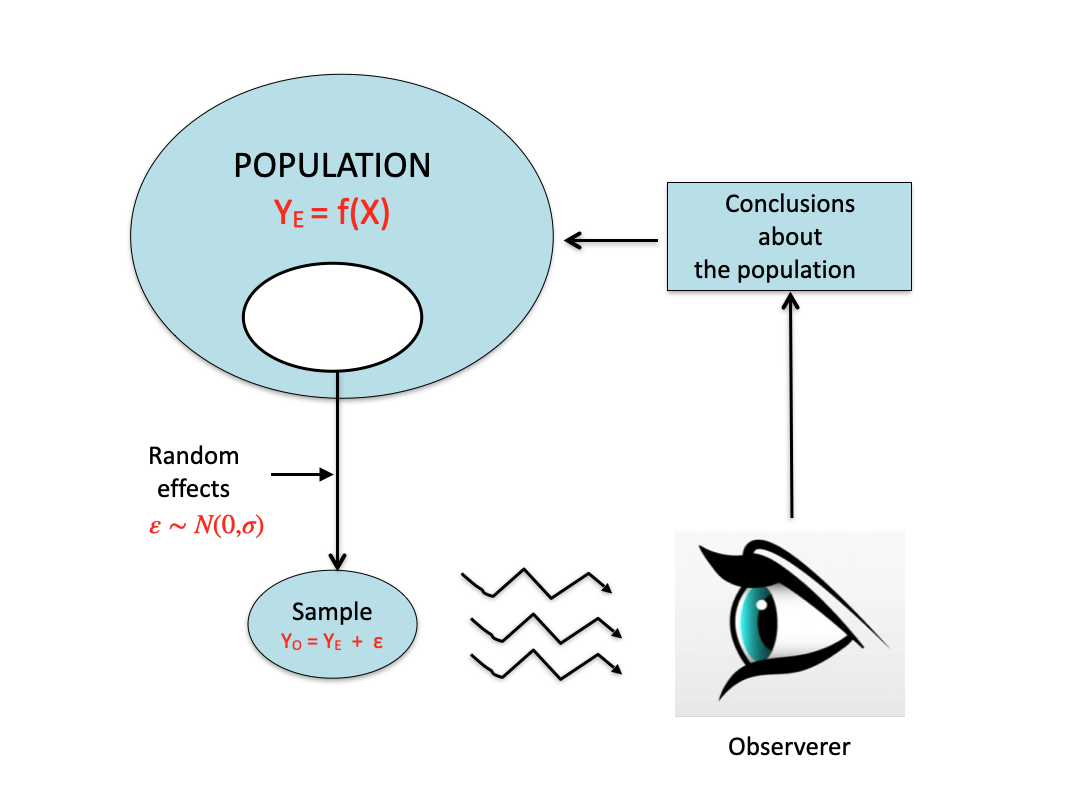
\includegraphics[width=0.75\linewidth]{_images/ExperimentalError} 

}

\caption{The process of experimental research: inferring the characteristics of a population by looking at a sample}\label{fig:figName61}
\end{figure}

In this chapter we will offer an overview about statistical inference, by using two real-life examples; the first one deals with a quantitative variable, while the second one deals with a proportion.

\hypertarget{example-1-a-concentration-value}{%
\section{Example 1: a concentration value}\label{example-1-a-concentration-value}}

Let's consider again the situation we have examined in Chapter 4: a well is polluted by herbicide residues and we want to know the concentration of those residues. We plan a Monte Carlo experiment where we collect three water samples and make chromatographic analyses.

As this is a Monte Carlo experiment, we can imagine that we know the real truth: the unknown concentration is 120 mg/L and the analytic instrument is characterised by a coefficient of variability of 10\%, corresponding to a standard deviation of 12 mg/L. Consequently, our observations (\(Y_i\), with \(i\) going from 1 to 3 replicates) will not match the real unknown concentration value, but they will be a random realisation, from the following Gaussian distribution (see Chapter 4):

\[Y_i \sim \textrm{Norm}(120, 12)\],

Accordingly, we can simulate the results of our experiment:

\begin{Shaded}
\begin{Highlighting}[]
\FunctionTok{set.seed}\NormalTok{(}\DecValTok{1234}\NormalTok{)}
\NormalTok{Ye }\OtherTok{\textless{}{-}} \DecValTok{120}
\NormalTok{Y }\OtherTok{\textless{}{-}} \FunctionTok{rnorm}\NormalTok{(}\DecValTok{3}\NormalTok{, Ye, }\DecValTok{12}\NormalTok{)}
\NormalTok{Y}
\DocumentationTok{\#\# [1] 105.5152 123.3292 133.0133}
\end{Highlighting}
\end{Shaded}

Now, let's put ourselves in the usual conditions: we have seen the results and we know nothing about the real truth. What can we learn from the data, about the concentration in the whole well?

First of all, we postulate a possible model, such as the usual model of the mean:

\[Y_i \sim \textrm{Norm}(\mu, \sigma)\]

This is the same model we used to simulate the experiment, but, in the real world, we do not know the values of \(\mu\) and \(\sigma\) and we need to estimate them from the observed data. We know that \(\mu\) and \(\sigma\) are, respectively, the mean and the standard deviation of the whole population and, therefore, we calculate these two descriptive stats for our sample and name them, respectively, \(m\) and \(s\).

\begin{Shaded}
\begin{Highlighting}[]
\NormalTok{m }\OtherTok{\textless{}{-}} \FunctionTok{mean}\NormalTok{(Y)}
\NormalTok{s }\OtherTok{\textless{}{-}} \FunctionTok{sd}\NormalTok{(Y)}
\NormalTok{m; s}
\DocumentationTok{\#\# [1] 120.6192}
\DocumentationTok{\#\# [1] 13.9479}
\end{Highlighting}
\end{Shaded}

Now the question is: having seen \(m\) and \(s\), can we infere the values of \(\mu\) and \(\sigma\)? Assuming that the sample is representative (we should not question this, as long as the experiment is valid), our best guess is that \(\mu = m\) and \(\sigma = s\). This process by which we assign the observed sample values to the population values is known as \textbf{point estimation}.

Although point estimation is totally legitimate, we clearly see that it leads to wrong conclusions: due to sampling errors, \(m\) is not exactly equal to \(\mu\) and \(s\) is not exactly equal to \(\sigma\)! Therefore, a more prudential attitude is recommended: instead of expressing our best guess as a single value, we would be much better off if we could use some sort of uncertainty interval. We need a heuristic to build such an interval.

\hypertarget{the-empirical-sampling-distribution}{%
\subsection{The empirical sampling distribution}\label{the-empirical-sampling-distribution}}

In this book we will use the popular heuristic proposed by Jarzy Neyman, although we need to clearly state that this is not the only one and it is not free from some conceptual inconsistencies (See Morey et al., 2016). Such a heuristic is based on trying to guess what should happen if we repeat the experiment for a very high number of times. Shall we obtain similar results or different? Instead of guessing, we exploit Monte Carlo simulation to make true repeats. Therefore:

\begin{enumerate}
\def\labelenumi{\arabic{enumi}.}
\tightlist
\item
  we repeat the sampling process 100,000 times (i.e., we collect three water samples for 100,000 times and analyse their concentrations)
\item
  we get 100,000 average concentration values
\item
  we describe this population of means.
\end{enumerate}

In R, we can use the code below. Please, note the iterative procedure, based on the \texttt{for()} statement, by which all instructions between curly brackets are repeated, while the counter \(i\) is updated at each cycle, from 1 to 100,000.

\begin{Shaded}
\begin{Highlighting}[]
\CommentTok{\# Monte Carlo simulation}
\FunctionTok{set.seed}\NormalTok{(}\DecValTok{1234}\NormalTok{)}
\NormalTok{result }\OtherTok{\textless{}{-}} \FunctionTok{rep}\NormalTok{(}\DecValTok{0}\NormalTok{, }\DecValTok{100000}\NormalTok{)}
\ControlFlowTok{for}\NormalTok{ (i }\ControlFlowTok{in} \DecValTok{1}\SpecialCharTok{:}\DecValTok{100000}\NormalTok{)\{}
\NormalTok{  sample }\OtherTok{\textless{}{-}} \FunctionTok{rnorm}\NormalTok{(}\DecValTok{3}\NormalTok{, }\DecValTok{120}\NormalTok{, }\DecValTok{12}\NormalTok{)}
\NormalTok{  result[i] }\OtherTok{\textless{}{-}} \FunctionTok{mean}\NormalTok{(sample)}
\NormalTok{\}}
\FunctionTok{mean}\NormalTok{(result)}
\DocumentationTok{\#\# [1] 120.0341}
\FunctionTok{sd}\NormalTok{(result)}
\DocumentationTok{\#\# [1] 6.939063}
\end{Highlighting}
\end{Shaded}

Now, we have a population of sample means and we see that:

\begin{enumerate}
\def\labelenumi{\arabic{enumi}.}
\tightlist
\item
  the mean of this population is equal to the mean of the original population. It is, therefore, confirmed that the only way to obtain a perfect estimate of the population mean \(\mu\) is to repeat the experiment an infinite number of times;
\item
  the standard deviation of the population of means is equal to 6.94 and it is called \textbf{standard error} (SE); this value is smaller than \(\sigma\).
\end{enumerate}

In order to more thouroughly describe the variability of sample means, we can bin the concentration values into a series of intervals (from 80 to 160 mg/L with a 2.5 step) and calculate the proportion of means in each interval. In this way, we build an empirical distribution of probabilities for the sample means (Figure \ref{fig:figName62}), which is called \textbf{sampling distribution}. Indeed, this term has a more general importance and it is used to name the distribution of probabilities for every possible sample statistics.

\begin{figure}

{\centering 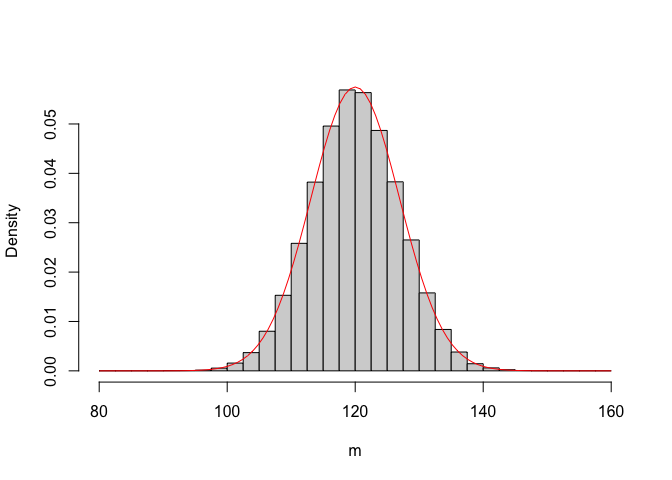
\includegraphics[width=0.9\linewidth]{_main_files/figure-latex/figName62-1} 

}

\caption{Empirical distribution of 100,000 sample means (n = 3) from a Gaussian population with mean = 120 and SD = 12. The solid line shows a Gaussian PDF, with mean = 120 and SD = 6.94}\label{fig:figName62}
\end{figure}

The sampling distribution and its standard error are two very important objects in research, as they are used to describe the precision of estimates: \textbf{when the standard error is big, the sampling distribution is flat and our estimates are tend to be rather uncertain and highly variable across repeated experiments. Otherwise, when the standard error is small, our estimates are very reliable and precise.}

\hypertarget{a-theoretical-sampling-distribution}{%
\subsection{A theoretical sampling distribution}\label{a-theoretical-sampling-distribution}}

Building an empirical sampling distribution by Monte Carlo simulation is always possible, but it may often be impractical. Looking at Figure \ref{fig:figName62}, we see that our sampling distribution looks very much like a Gaussian PDF with mean equal to 120 and standard deviation close to 6.94.

Indeed, such an empirical observation has a theoretical support: the \textbf{central limit theorem} states that the sampling distribution of whatever statistic obtained from random and independent samples is approximately gaussian, whatever it is the PDF of the original population where we sampled from.\footnote{The central limit theorem holds for very large samples. With small samples, the approximation is good only with more than 15-20 units} The same theorem proves that, if the population mean is \(\mu\), the mean of the sampling distribution is \(\mu\).

The standard deviation of the sampling distribution, in this case, can be derived by the law of propagation of errors, based on three main rules:

\begin{enumerate}
\def\labelenumi{\arabic{enumi}.}
\tightlist
\item
  the sum of gaussian variables is also gaussian. Besides, the product of a gaussian variable for a constant value is also gaussian.
\item
  For independent gaussian variables, the mean of the sum is equal to the sum of the means and the variance of the sum is equal to the sum of the variances.
\item
  If we take a gaussian variable with mean equal to \(\mu\) and variance equal to \(\sigma^2\) and multiply all individuals by a constant value \(k\), the mean of the product is equal to \(k \times \mu\), while the variance is \(k^2 \times \sigma^2\).
\end{enumerate}

In our experiment, we have three individuals coming from a gaussian distribution and each individual inherits the variance of the population from which it was sampled, which is \(\sigma^2 = 12^2 = 144\). When we calculate the mean, we sum the three values as the first step and the variance of the sum is \(144 + 144 + 144 = 3 \times 144 = 432\). As the second step, we divide by three and the variance of this ratio (see \#3 above) is 432 divided by \(3^2\), i.e.~\(432/9 = 48\). The standard error is, therefore, \(\sqrt{48} = 6.928\); it is not exactly equal to the empirical value of 9.94, but this is only due to the fact that we did not make an infinite number of repeated sampling.

In general, the standard error of a mean (SEM) is:

\[\sigma_m  = \frac{\sigma}{\sqrt n}\]

Now, we can make our first conclusion: \textbf{if we repeat an experiment a very high number of times, the variability of results across replicates can be described by a sampling distribution, that is (approximately) gaussian, with mean equal to the true result of our experiment and standard deviation equal to the standard error.}

\hypertarget{the-frequentist-confidence-interval}{%
\subsection{The frequentist confidence interval}\label{the-frequentist-confidence-interval}}

If the sampling distribution is gaussian, we could take a value \(k\), so that the following expression holds:

\[P \left[ \mu - k \times \frac{\sigma}{\sqrt{n} } \leq m \leq \mu + k \times \frac{\sigma}{\sqrt{n} } \right] = 0.95\]

It means that we can build an interval around \(\mu\) that contains 95\% of the sample means (\(m\)) from repeated experiments (Figure \ref{fig:figName62b}).

\begin{figure}

{\centering 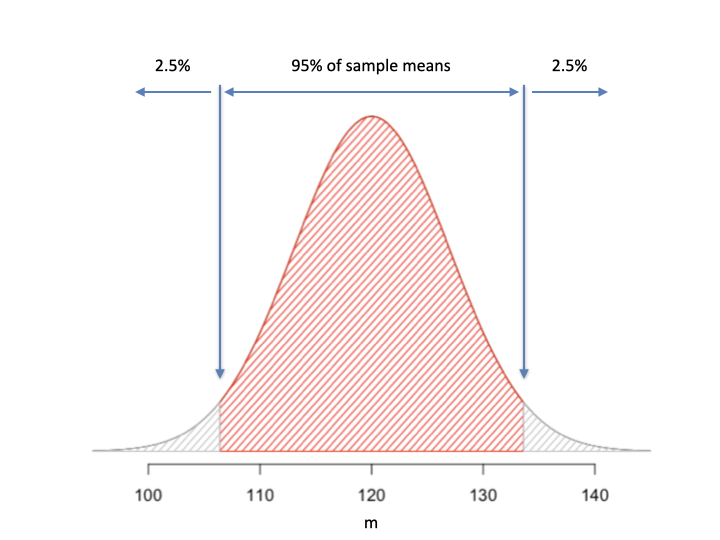
\includegraphics[width=0.9\linewidth]{_images/ConfidenceInterval} 

}

\caption{Building a confidence interval (P = 0.95): if we sample from a population with a mean of 120, 95 of our sample means out of 100 will be in the above interval}\label{fig:figName62b}
\end{figure}

With simple math, we get to the following expression, that is of extreme importance:

\[P \left[ m - k \times \frac{\sigma}{\sqrt{n} } \leq \mu \leq m + k \times \frac{\sigma}{\sqrt{n} } \right] = 0.95\]

It says that, \textbf{when we make an experiment and get an estimate \(m\), by an appropriate selection of \(k\), we can build an interval around \(m\) that is equal to \(k\) times the standard error, and contains the population value \(\mu\) with 95\% probability}. Here is the heuristic we were looking for!

For our example:

\begin{enumerate}
\def\labelenumi{\arabic{enumi}.}
\tightlist
\item
  we calculate the sample mean. We conclude that \(\mu = m = 120.6192\) mg/L and this is our point estimate;
\item
  we calculate the standard error as \(\sigma/\sqrt{n}\). As we do not know \(\sigma\), we plug-in our best guess, that is \(s = 13.95\), so that \(SE = 13.95 / \sqrt{3} = 8.053\);
\item
  we express our uncertainty about the population mean by replacing the point estimate with an interval, given by \(\mu = 120.6192 \pm k \times 8.053\). This process is known as \textbf{interval estimation}.
\end{enumerate}

The interval \(\mu = 120.6192 \pm k \times 8.053\) is called \textbf{confidence interval} and it is supposed to give us a better confidence that we are not reporting a wrong mean for the population (be careful to this: we are in doubt about the population, not about the sample!).

But, how do we select a value for the multiplier \(k\)? Let's go by trial and error. We set \(k = 1\) and repeat our Monte Carlo simulations, as we did before. At this time, we calculate 100,000 confidence intervals and count the number of cases where we hit the population mean. The code is shown below and it is very similar to the code we previously used to build our sampling distribution.

\begin{Shaded}
\begin{Highlighting}[]
\CommentTok{\# Monte Carlo simulation {-} 2}
\FunctionTok{set.seed}\NormalTok{(}\DecValTok{1234}\NormalTok{)}
\NormalTok{result }\OtherTok{\textless{}{-}} \FunctionTok{rep}\NormalTok{(}\DecValTok{0}\NormalTok{, }\DecValTok{100000}\NormalTok{)}
\ControlFlowTok{for}\NormalTok{ (i }\ControlFlowTok{in} \DecValTok{1}\SpecialCharTok{:}\DecValTok{100000}\NormalTok{)\{}
\NormalTok{  sample }\OtherTok{\textless{}{-}} \FunctionTok{rnorm}\NormalTok{(}\DecValTok{3}\NormalTok{, }\DecValTok{120}\NormalTok{, }\DecValTok{12}\NormalTok{)}
\NormalTok{  m }\OtherTok{\textless{}{-}} \FunctionTok{mean}\NormalTok{(sample)}
\NormalTok{  se }\OtherTok{\textless{}{-}} \FunctionTok{sd}\NormalTok{(sample)}\SpecialCharTok{/}\FunctionTok{sqrt}\NormalTok{(}\DecValTok{3}\NormalTok{)}
\NormalTok{  limInf }\OtherTok{\textless{}{-}}\NormalTok{ m }\SpecialCharTok{{-}}\NormalTok{ se}
\NormalTok{  limSup }\OtherTok{\textless{}{-}}\NormalTok{ m }\SpecialCharTok{+}\NormalTok{ se}
  \ControlFlowTok{if}\NormalTok{(limInf }\SpecialCharTok{\textless{}} \DecValTok{120} \SpecialCharTok{\&}\NormalTok{ limSup }\SpecialCharTok{\textgreater{}} \DecValTok{120}\NormalTok{) result[i] }\OtherTok{\textless{}{-}} \DecValTok{1}
\NormalTok{\}}
\FunctionTok{sum}\NormalTok{(result)}\SpecialCharTok{/}\DecValTok{100000}
\DocumentationTok{\#\# [1] 0.57749}
\end{Highlighting}
\end{Shaded}

Indeed, we hit the real population mean only in less than 60 cases out of 100, which is very far away from 95\%; we'd better widen our interval. If we use twice the standard error (\(k = 2\)), the probability becomes slightly higher than 81\% (try to run the code below).

\begin{Shaded}
\begin{Highlighting}[]
\CommentTok{\# Monte Carlo simulation {-} 3}
\FunctionTok{set.seed}\NormalTok{(}\DecValTok{1234}\NormalTok{)}
\NormalTok{result }\OtherTok{\textless{}{-}} \FunctionTok{rep}\NormalTok{(}\DecValTok{0}\NormalTok{, }\DecValTok{100000}\NormalTok{)}
\ControlFlowTok{for}\NormalTok{ (i }\ControlFlowTok{in} \DecValTok{1}\SpecialCharTok{:}\DecValTok{100000}\NormalTok{)\{}
\NormalTok{  sample }\OtherTok{\textless{}{-}} \FunctionTok{rnorm}\NormalTok{(}\DecValTok{3}\NormalTok{, }\DecValTok{120}\NormalTok{, }\DecValTok{12}\NormalTok{)}
\NormalTok{  m }\OtherTok{\textless{}{-}} \FunctionTok{mean}\NormalTok{(sample)}
\NormalTok{  se }\OtherTok{\textless{}{-}} \FunctionTok{sd}\NormalTok{(sample)}\SpecialCharTok{/}\FunctionTok{sqrt}\NormalTok{(}\DecValTok{3}\NormalTok{)}
\NormalTok{  limInf }\OtherTok{\textless{}{-}}\NormalTok{ m }\SpecialCharTok{{-}} \DecValTok{2} \SpecialCharTok{*}\NormalTok{ se}
\NormalTok{  limSup }\OtherTok{\textless{}{-}}\NormalTok{ m }\SpecialCharTok{+} \DecValTok{2} \SpecialCharTok{*}\NormalTok{ se}
  \ControlFlowTok{if}\NormalTok{(limInf }\SpecialCharTok{\textless{}} \DecValTok{120} \SpecialCharTok{\&}\NormalTok{ limSup }\SpecialCharTok{\textgreater{}} \DecValTok{120}\NormalTok{) result[i] }\OtherTok{\textless{}{-}} \DecValTok{1}
\NormalTok{\}}
\FunctionTok{sum}\NormalTok{(result)}\SpecialCharTok{/}\DecValTok{100000}
\DocumentationTok{\#\# [1] 0.81708}
\end{Highlighting}
\end{Shaded}

Using twice the standard error could be a good approximation when we have a high number of degrees of freedom. For example, running the code below shows that, with 20 replicates, a confidence interval obtained as \(m \pm 2 \times s/\sqrt{3}\) hits the population mean in more than 94\% of the cases. Therefore, such a confidence interval (`naive' confidence interval) is simple and it is a good approximation to the 95\% confidence interval when the number of observations is sufficiently high.

\begin{Shaded}
\begin{Highlighting}[]
\CommentTok{\# Monte Carlo simulation {-} 4}
\FunctionTok{set.seed}\NormalTok{(}\DecValTok{1234}\NormalTok{)}
\NormalTok{result }\OtherTok{\textless{}{-}} \FunctionTok{rep}\NormalTok{(}\DecValTok{0}\NormalTok{, }\DecValTok{100000}\NormalTok{)}
\ControlFlowTok{for}\NormalTok{ (i }\ControlFlowTok{in} \DecValTok{1}\SpecialCharTok{:}\DecValTok{100000}\NormalTok{)\{}
\NormalTok{  n }\OtherTok{\textless{}{-}} \DecValTok{20}
\NormalTok{  sample }\OtherTok{\textless{}{-}} \FunctionTok{rnorm}\NormalTok{(n, }\DecValTok{120}\NormalTok{, }\DecValTok{12}\NormalTok{)}
\NormalTok{  m }\OtherTok{\textless{}{-}} \FunctionTok{mean}\NormalTok{(sample)}
\NormalTok{  se }\OtherTok{\textless{}{-}} \FunctionTok{sd}\NormalTok{(sample)}\SpecialCharTok{/}\FunctionTok{sqrt}\NormalTok{(n)}
\NormalTok{  limInf }\OtherTok{\textless{}{-}}\NormalTok{ m }\SpecialCharTok{{-}} \DecValTok{2} \SpecialCharTok{*}\NormalTok{ se}
\NormalTok{  limSup }\OtherTok{\textless{}{-}}\NormalTok{ m }\SpecialCharTok{+} \DecValTok{2} \SpecialCharTok{*}\NormalTok{ se}
  \ControlFlowTok{if}\NormalTok{(limInf }\SpecialCharTok{\textless{}} \DecValTok{120} \SpecialCharTok{\&}\NormalTok{ limSup }\SpecialCharTok{\textgreater{}} \DecValTok{120}\NormalTok{) result[i] }\OtherTok{\textless{}{-}} \DecValTok{1}
\NormalTok{\}}
\FunctionTok{sum}\NormalTok{(result)}\SpecialCharTok{/}\DecValTok{100000}
\DocumentationTok{\#\# [1] 0.94099}
\end{Highlighting}
\end{Shaded}

For our small sample case, we can get an exact 95\% coverage by using the 97.5-th percentile of a Student's t distribution, that is calculated by using the \texttt{qt()} function in R:

\begin{Shaded}
\begin{Highlighting}[]
\FunctionTok{qt}\NormalTok{(}\FloatTok{0.975}\NormalTok{, }\DecValTok{2}\NormalTok{)}
\DocumentationTok{\#\# [1] 4.302653}
\end{Highlighting}
\end{Shaded}

The first argument is the desired percentile, while the second argument represents the number of degrees of freedom for the standard deviation of the sample, that is \(n - 1\). The value of 4.303 can be used as the multiplier for the standard error, leading to the following confidence limits:

\begin{Shaded}
\begin{Highlighting}[]
\NormalTok{m }\SpecialCharTok{+} \FunctionTok{qt}\NormalTok{(}\FloatTok{0.025}\NormalTok{, }\DecValTok{2}\NormalTok{) }\SpecialCharTok{*}\NormalTok{ s}\SpecialCharTok{/}\FunctionTok{sqrt}\NormalTok{(}\DecValTok{3}\NormalTok{)}
\DocumentationTok{\#\# [1] 85.33977}
\NormalTok{m }\SpecialCharTok{+} \FunctionTok{qt}\NormalTok{(}\FloatTok{0.975}\NormalTok{, }\DecValTok{2}\NormalTok{) }\SpecialCharTok{*}\NormalTok{ s}\SpecialCharTok{/}\FunctionTok{sqrt}\NormalTok{(}\DecValTok{3}\NormalTok{)}
\DocumentationTok{\#\# [1] 154.6368}
\end{Highlighting}
\end{Shaded}

A further Monte Carlo simulation (see below) shows that this is a good heuristic, as it gives us a confidence interval with a real 95\% coverage.

\begin{Shaded}
\begin{Highlighting}[]
\CommentTok{\# Monte Carlo simulation {-} 4}
\FunctionTok{set.seed}\NormalTok{(}\DecValTok{1234}\NormalTok{)}
\NormalTok{result }\OtherTok{\textless{}{-}} \FunctionTok{rep}\NormalTok{(}\DecValTok{0}\NormalTok{, }\DecValTok{100000}\NormalTok{)}
\ControlFlowTok{for}\NormalTok{ (i }\ControlFlowTok{in} \DecValTok{1}\SpecialCharTok{:}\DecValTok{100000}\NormalTok{)\{}
\NormalTok{  sample }\OtherTok{\textless{}{-}} \FunctionTok{rnorm}\NormalTok{(}\DecValTok{3}\NormalTok{, }\DecValTok{120}\NormalTok{, }\DecValTok{12}\NormalTok{)}
\NormalTok{  m }\OtherTok{\textless{}{-}} \FunctionTok{mean}\NormalTok{(sample)}
\NormalTok{  se }\OtherTok{\textless{}{-}} \FunctionTok{sd}\NormalTok{(sample)}\SpecialCharTok{/}\FunctionTok{sqrt}\NormalTok{(}\DecValTok{3}\NormalTok{)}
\NormalTok{  limInf }\OtherTok{\textless{}{-}}\NormalTok{ m }\SpecialCharTok{{-}} \FunctionTok{qt}\NormalTok{(}\FloatTok{0.975}\NormalTok{, }\DecValTok{2}\NormalTok{) }\SpecialCharTok{*}\NormalTok{ se}
\NormalTok{  limSup }\OtherTok{\textless{}{-}}\NormalTok{ m }\SpecialCharTok{+} \FunctionTok{qt}\NormalTok{(}\FloatTok{0.975}\NormalTok{, }\DecValTok{2}\NormalTok{) }\SpecialCharTok{*}\NormalTok{ se}
  \ControlFlowTok{if}\NormalTok{(limInf }\SpecialCharTok{\textless{}} \DecValTok{120} \SpecialCharTok{\&}\NormalTok{ limSup }\SpecialCharTok{\textgreater{}} \DecValTok{120}\NormalTok{) result[i] }\OtherTok{\textless{}{-}} \DecValTok{1}
\NormalTok{\}}
\FunctionTok{sum}\NormalTok{(result)}\SpecialCharTok{/}\DecValTok{100000}
\DocumentationTok{\#\# [1] 0.94936}
\end{Highlighting}
\end{Shaded}

Obviously, we can also build a 99\% or whatever else confidence interval, we only have to select the right percentile from a Student's t distribution. In general, if \(\alpha\) is the confidence level (e.g.~0.95 or 0.99), the percentile is \(1 - (1 - \alpha)/2\) (e.g., \(1 - (1 - 0.95)/2 = 0.975\) or \(1 - (1 - 0.99)/2 = 0.995\)).

\hypertarget{example-2-a-proportion}{%
\section{Example 2: a proportion}\label{example-2-a-proportion}}

For the previous example, we have sampled from a gaussian population, but this is not always true. Let's imagine we have a population of seeds, which are 77.5\% germinable and 22.5\% dormant. If we take a sample of 40 seeds and measure their germinability, we should not necessarily obtain 31 (40 \(\times\) 0.775) germinated seeds, due to random sample-to-sample fluctuations.

Analogously to the previous example, we could think that the number of germinated seeds might show random variability, according to a gaussian PDF with \(\mu\) = 31 and a certain standard deviation \(\sigma\). However, such an assumption is not reasonable: the count of germinated seeds is a discrete variable going from 0 to 40, while the gaussian PDF is continuous from \(-\infty\) to \(\infty\). A survey of literature shows that the random variability in the number of germinated seeds can be described by using a binomial PDF (Snedecor and Cochran, 1989); accordingly, we can simulate our germination experiment by using a binomial random number generator, that is the \texttt{rbinom(s,\ n,\ p)} function. The first argument represents the number of experiments we intend to request, the second represents the number of seeds under investigation in each experiment, while the third one represents the proportion of successes in the population (we can take the germination as a success). Let's simulate the results of an experiment:

\begin{Shaded}
\begin{Highlighting}[]
\FunctionTok{set.seed}\NormalTok{(}\DecValTok{1234}\NormalTok{)}
\NormalTok{nGerm }\OtherTok{\textless{}{-}} \FunctionTok{rbinom}\NormalTok{(}\DecValTok{1}\NormalTok{, }\DecValTok{40}\NormalTok{, }\FloatTok{0.775}\NormalTok{)}
\NormalTok{nGerm}
\DocumentationTok{\#\# [1] 34}
\NormalTok{nGerm}\SpecialCharTok{/}\DecValTok{40}
\DocumentationTok{\#\# [1] 0.85}
\end{Highlighting}
\end{Shaded}

We see that we get 34 germinated seeds, corresponding to a proportion \(p = 34/40 = 0.85\). Looking at the observed data, what can we conclude about the proportion of germinable seeds for the whole population? Our point estimate, as usual, is \(\pi = p = 0.85\), but we see that this is expectedly wrong; how could we calculate a confidence interval around this point estimate? Can we use the same heuristic as we did before for concentration data?

Let's use Monte Carlo simulation to explore the empirical sampling distribution. We repeat the experiment 100,000 times and we obtain 100,000 proportions with which we build an empirical sampling distribution (see the code below, showing the sampled proportions for the first six experiment). How does the sampling distribution look like?

\begin{Shaded}
\begin{Highlighting}[]
\NormalTok{res }\OtherTok{\textless{}{-}} \FunctionTok{rbinom}\NormalTok{(}\DecValTok{100000}\NormalTok{, }\DecValTok{40}\NormalTok{, }\FloatTok{0.775}\NormalTok{)}\SpecialCharTok{/}\DecValTok{40}
\FunctionTok{head}\NormalTok{(res)}
\DocumentationTok{\#\# [1] 0.750 0.750 0.750 0.700 0.750 0.925}
\FunctionTok{mean}\NormalTok{(res)}
\DocumentationTok{\#\# [1] 0.7749263}
\FunctionTok{sd}\NormalTok{(res)}
\DocumentationTok{\#\# [1] 0.06611151}
\end{Highlighting}
\end{Shaded}

Unsurprisingly, Monte Carlo simulation leads us to an approximately normal sampling distribution for \(p\), as implied by the central limit theorem (Figure \ref{fig:figName62c}). Furthermore, the mean of the sampling distribution is 0.775 and the standard deviation is 0.066.

\begin{figure}

{\centering 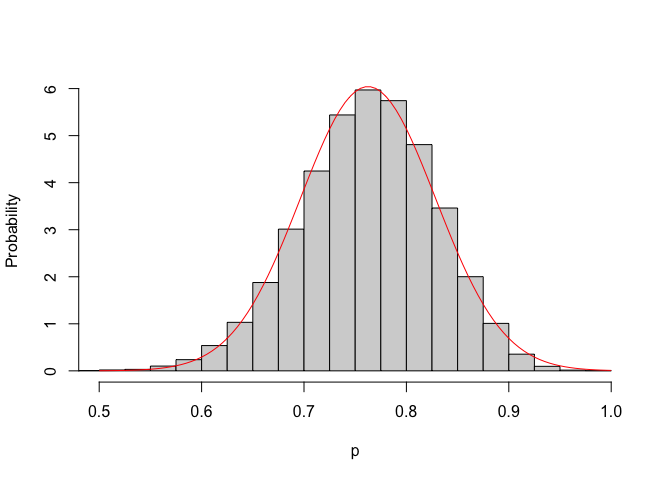
\includegraphics[width=0.9\linewidth]{_main_files/figure-latex/figName62c-1} 

}

\caption{Monte Carlo sampling distribution for the proportion of germinable seeds, when the population proportion is 0.775}\label{fig:figName62c}
\end{figure}

We can conclude that the confidence interval for an estimated proportion can be calculated in the very same way as for the mean, with the only difference that the standard error is obtained as \(\sigma_p = \sqrt{p \times (1 - p)}/\sqrt(n)\) (Snedecor and Cochran, 1989). Consequently, using the observed data, \(p = 0.85\) and \(s = \sqrt{0.85 \times 0.15} = 0.357\); our confidence interval is \(0.85 \pm 2 \times 0.357/sqrt(40)\) and we can see that, by reporting such an interval, we have correctly hit our population proportion. In this case the size of our sample was big enough (40) to use \(k = 2\) as the multiplier.

\hypertarget{conclusions-2}{%
\section{Conclusions}\label{conclusions-2}}

The examples we used are rather simple, but they should help to understand the process:

\begin{enumerate}
\def\labelenumi{\arabic{enumi}.}
\tightlist
\item
  we have a population, from which we sampled the observed data;
\item
  we used the observed data to calculate a statistic (mean or proportion);
\item
  we inferred that the population statistic was equal to the sample statistic (e.g., \(\mu = m\) or \(\pi = p\));
\item
  we estimated a standard error for our sample statistic, by using either Monte Carlo simulation, or by using some simple function, depending on the selected statistic (e.g.~\(\sigma/\sqrt{n}\) for the mean and \(\sqrt{p \times (1 - p)}/\sqrt(n)\) for the proportion);
\item
  we used a multiple of the standard error to build a confidence interval around our point estimate.
\end{enumerate}

We will use the same process throughout this book, although the sample statistics and related standard errors will become slightly more complex, as we progress towards the end. \textbf{Please, do not forget that the standard error and confidence interval are fundamental components of science and should always be reported along with every point estimate}.

Last, but not least, it is important to put our attention on the meaning of the so-called `frequentist' confidence interval:

\begin{enumerate}
\def\labelenumi{\arabic{enumi}.}
\tightlist
\item
  it is a measure of precision
\item
  it relates to the sampling distribution; i.e.~we say that, if we repeat the experiment a high number of times and, at any times, we calculate the confidence interval as shown above, we `capture' the real unknown parameter value in 95\% of the cases
\item
  it does not refer to a single sampling effort
\end{enumerate}

Points 2 and 3 above imply that confidence intervals protect ourselves from the risk of reaching wrong conclusions only in the long run. In other words, the idea is that, if we use such a heuristic, we will not make too many mistakes in our research life, but that does not imply that we are 95\% correct in each experimental effort. Indeed, a single confidence interval may contain or not the true population mean, but we have no hint to understand whether we hit it or not. Therefore, please, remember that such expressions as: ``there is 95\% probability that the true population parameter is within the confidence interval'' are just abused and they should never find their way in any scientific manuscripts or reports.

\begin{center}\rule{0.5\linewidth}{0.5pt}\end{center}

\hypertarget{further-readings-3}{%
\section{Further readings}\label{further-readings-3}}

\begin{enumerate}
\def\labelenumi{\arabic{enumi}.}
\tightlist
\item
  Hastie, T., Tibshirani, R., Friedman, J., 2009. The elements of statistical learning, Springer Series in Statistics. Springer Science + Business Media, California, USA.
\item
  Morey, RD, R Hoekstra, JN Rouder, MD Lee, E-J Wagenmakers, 2016. The fallacy of placing confidence in confidence intervals. Psychonomic Bulletin \& Review 23, 103--123
\item
  Snedecor G.W. and Cochran W.G., 1989. Statistical Methods. Ames: Iowa State University Press (1989).
\end{enumerate}

\hypertarget{making-decisions-under-uncertainty}{%
\chapter{Making Decisions under uncertainty}\label{making-decisions-under-uncertainty}}

In Chapter 5 we have seen that experimental errors and, above all, sampling errors, produce uncertainty in the estimation process, which we have to account for by determining and displaying standard errors and confidence intervals. In the very same fashion, we need to be able to make decisions in presence of uncertainty; is the effect of a treatment statistically significant? Is the effect of a treatment higher/lower than the effect of another treatment?

Making such decisions is called \textbf{Formal Hypothesis Testing} (FHT) and we will see that this is mainly based on the so-called \textbf{P-value}. As usual, I will introduce the problem by using an example.

\hypertarget{comparing-sample-means-the-students-t-test}{%
\section{Comparing sample means: the Student's t-test}\label{comparing-sample-means-the-students-t-test}}

\hypertarget{the-dataset}{%
\subsection{The dataset}\label{the-dataset}}

We have planned an experiment where we have compared the yield of genotype A with the yield of the genotype P and the experiment is laid down according to a completely randomised design with five replicates. This is a small-plot experiment with 10 plots, which need to be regarded as sampled from a wider population of plots; as we mentioned in the previous chapter, our interest is not in the sample, but it is in the population of plots, which means that we are looking for conclusions of general validity.

The results (in quintals per hectare) are the following:

\begin{Shaded}
\begin{Highlighting}[]
\NormalTok{A }\OtherTok{\textless{}{-}} \FunctionTok{c}\NormalTok{(}\DecValTok{65}\NormalTok{, }\DecValTok{68}\NormalTok{, }\DecValTok{69}\NormalTok{, }\DecValTok{71}\NormalTok{, }\DecValTok{78}\NormalTok{)}
\NormalTok{P }\OtherTok{\textless{}{-}} \FunctionTok{c}\NormalTok{(}\DecValTok{80}\NormalTok{, }\DecValTok{81}\NormalTok{, }\DecValTok{84}\NormalTok{, }\DecValTok{88}\NormalTok{, }\DecValTok{94}\NormalTok{)}
\end{Highlighting}
\end{Shaded}

As usual we calculate the descriptive statistics (mean and standard deviation) for each sample:

\begin{Shaded}
\begin{Highlighting}[]
\NormalTok{mA }\OtherTok{\textless{}{-}} \FunctionTok{mean}\NormalTok{(A)}
\NormalTok{mP }\OtherTok{\textless{}{-}} \FunctionTok{mean}\NormalTok{(P)}
\NormalTok{sA }\OtherTok{\textless{}{-}} \FunctionTok{sd}\NormalTok{(A)}
\NormalTok{sP }\OtherTok{\textless{}{-}} \FunctionTok{sd}\NormalTok{(P)}
\NormalTok{mA; sA}
\DocumentationTok{\#\# [1] 70.2}
\DocumentationTok{\#\# [1] 4.868265}
\NormalTok{mP; sP}
\DocumentationTok{\#\# [1] 85.4}
\DocumentationTok{\#\# [1] 5.727128}
\end{Highlighting}
\end{Shaded}

We see that the mean for the genotype P is higher than the mean for the genotype A, but such descriptive statistics are not sufficient to our aims. Therefore, we calculate standard errors, to express our uncertainty about the population means, as we have shown in the previous chapter.

\begin{Shaded}
\begin{Highlighting}[]
\NormalTok{seA }\OtherTok{\textless{}{-}}\NormalTok{ sA}\SpecialCharTok{/}\FunctionTok{sqrt}\NormalTok{(}\DecValTok{5}\NormalTok{); seA}
\DocumentationTok{\#\# [1] 2.177154}
\NormalTok{seP }\OtherTok{\textless{}{-}}\NormalTok{ sP}\SpecialCharTok{/}\FunctionTok{sqrt}\NormalTok{(}\DecValTok{5}\NormalTok{); seP}
\DocumentationTok{\#\# [1] 2.56125}
\end{Highlighting}
\end{Shaded}

Consequently, we can produce interval estimates for the population means, i.e., 85.4 \(\pm\) 5.12 and 70.2 \(\pm\) 4.35. We note that the confidence intervals do not overlap, which supports the idea that P is better than A, but we would like to reach a more formal decision.

First of all, we can see that the observed difference between \(m_A\) and \(m_P\) is equal to:

\begin{Shaded}
\begin{Highlighting}[]
\NormalTok{mA }\SpecialCharTok{{-}}\NormalTok{ mP}
\DocumentationTok{\#\# [1] {-}15.2}
\end{Highlighting}
\end{Shaded}

However, we are not interested in the above difference, but we are interested in the population difference, i.e.~\(\mu_A - \mu_P\). We know that both the means have a certain degree of uncertainty, which propagates to the difference. In the previous chapter, we have seen that the variance of the sum/difference of independent samples is equal to the sum of variances; therefore, the standard error of the difference (SED) is equal to:

\[SED = \sqrt{ SEM_1^2 + SEM_2^2 }\]

In our example, the SED is:

\begin{Shaded}
\begin{Highlighting}[]
\NormalTok{SED }\OtherTok{\textless{}{-}} \FunctionTok{sqrt}\NormalTok{(seA}\SpecialCharTok{\^{}}\DecValTok{2} \SpecialCharTok{+}\NormalTok{ seP}\SpecialCharTok{\^{}}\DecValTok{2}\NormalTok{)}
\NormalTok{SED}
\DocumentationTok{\#\# [1] 3.361547}
\end{Highlighting}
\end{Shaded}

It is intuitively clear that the difference (in quintals per hectare) should be regarded as significant when it is much higher than its standard error; indeed, this would mean that the difference is stronger than the uncertainty with which we have estimated it. We can formalise such an intuition by defining the \(T\) statistic for the sample difference:

\[T = \frac{m_A - m_P}{SED}\]

which is equal to:

\begin{Shaded}
\begin{Highlighting}[]
\NormalTok{Ti }\OtherTok{\textless{}{-}}\NormalTok{ (mA }\SpecialCharTok{{-}}\NormalTok{ mP)}\SpecialCharTok{/}\NormalTok{SED}
\NormalTok{Ti}
\DocumentationTok{\#\# [1] {-}4.521727}
\end{Highlighting}
\end{Shaded}

If T is big, the difference is likely to be significant (not due to random effects); however, \(T\) is a sample statistic and it is expected to change whenever we repeat the experiment. How is the sampling distribution for \(T\)? To answer this question, we should distinguish two possible hypotheses about the data:

\begin{itemize}
\tightlist
\item
  Hypothesis 1. There is no difference between the two genotypes (\textbf{null hypothesis}: \(H_0\)) and, consequently, we have only one population and the two samples A and P are extracted from this population.
\item
  Hypothesis 2. The two genotypes are different (\textbf{alternative hypothesis}: \(H_1\)) and, consequently, the two samples are extracted from two different populations, one for the A genotype and the other one for the P genotype.
\end{itemize}

In mathematical terms, the null hypothesis is:

\[H_0: \mu_1 = \mu_2 = \mu\]

The alternative hypothesis is:

\[H_1 :\mu_1  \neq \mu_2\]

More complex alternative hypotheses are also possible, such as \(H_1 :\mu _1 > \mu _2\), or \(H_1 :\mu _1 < \mu _2\). However, hypotheses should be set before looking at the data (according to the Galilean principle) and, in this case, we have no prior knowledge to justify the selection of one of such complex hypotheses. Therefore, we select the simple alternative hypothesis.

Which of the two hypotheses is more reasonable, by considering the observed data? We have seen that, \textbf{according to the Popperian falsification principle, experiments should be planned to falsify hypotheses. Therefore, we take the null hypothesis and see whether we can falsify it.}

This is one hint: if the null hypothesis were true, we should observe \(T = 0\), while we have observed \(T = -4.521727\). Is this enough to reject the null? Not at all, obviously. Indeed, the sample means can change from one experiment to the other and it is possible to obtain \(T \neq 0\) also when the experimental treatments are, indeed, the same treatment. Therefore, we need to ask ourselves: \textbf{what is the sampling distribution for \(T\) under the null hypothesis?}

\hypertarget{monte-carlo-simulation}{%
\subsection{Monte Carlo simulation}\label{monte-carlo-simulation}}

We can easily build an empirical sampling distribution for \(T\) by using Monte Carlo simulation. Look at the code in the box below: we use the \texttt{for()} statement to repeat the experiment 100,000 times. Each experiment consists of getting two samples of five individuals from the same population, with mean and standard deviation equal to the overall mean/standard deviation of the two original samples A and P. For each of the 100,000 couples of samples, we calculate T and store the result in the `result' vector, which, in the end, represents the sampling distribution we were looking for.

\begin{Shaded}
\begin{Highlighting}[]
\CommentTok{\# We assume a single population}
\NormalTok{mAP }\OtherTok{\textless{}{-}} \FunctionTok{mean}\NormalTok{(}\FunctionTok{c}\NormalTok{(A, P))}
\NormalTok{devStAP }\OtherTok{\textless{}{-}} \FunctionTok{sd}\NormalTok{(}\FunctionTok{c}\NormalTok{(A, P))}

\CommentTok{\# we repeatedly sample from this common population}
\FunctionTok{set.seed}\NormalTok{(}\DecValTok{34}\NormalTok{)}
\NormalTok{result }\OtherTok{\textless{}{-}} \FunctionTok{rep}\NormalTok{(}\DecValTok{0}\NormalTok{, }\DecValTok{100000}\NormalTok{)}
\ControlFlowTok{for}\NormalTok{ (i }\ControlFlowTok{in} \DecValTok{1}\SpecialCharTok{:}\DecValTok{100000}\NormalTok{)\{}
\NormalTok{  sample1 }\OtherTok{\textless{}{-}} \FunctionTok{rnorm}\NormalTok{(}\DecValTok{5}\NormalTok{, mAP, devStAP)}
\NormalTok{  sample2 }\OtherTok{\textless{}{-}} \FunctionTok{rnorm}\NormalTok{(}\DecValTok{5}\NormalTok{, mAP, devStAP)}
\NormalTok{  SED }\OtherTok{\textless{}{-}} \FunctionTok{sqrt}\NormalTok{( (}\FunctionTok{sd}\NormalTok{(sample1)}\SpecialCharTok{/}\FunctionTok{sqrt}\NormalTok{(}\DecValTok{5}\NormalTok{))}\SpecialCharTok{\^{}}\DecValTok{2} \SpecialCharTok{+}
\NormalTok{                 (}\FunctionTok{sd}\NormalTok{(sample2)}\SpecialCharTok{/}\FunctionTok{sqrt}\NormalTok{(}\DecValTok{5}\NormalTok{))}\SpecialCharTok{\^{}}\DecValTok{2}\NormalTok{ )}
\NormalTok{  result[i] }\OtherTok{\textless{}{-}}\NormalTok{ (}\FunctionTok{mean}\NormalTok{(sample1) }\SpecialCharTok{{-}} \FunctionTok{mean}\NormalTok{(sample2)) }\SpecialCharTok{/}\NormalTok{ SED}
\NormalTok{\}}
\FunctionTok{mean}\NormalTok{(result) }
\DocumentationTok{\#\# [1] {-}0.001230418}
\FunctionTok{min}\NormalTok{(result)}
\DocumentationTok{\#\# [1] {-}9.993187}
\FunctionTok{max}\NormalTok{(result)}
\DocumentationTok{\#\# [1] 9.988315}
\end{Highlighting}
\end{Shaded}

What values did we obtain for \(T\)? On average, the values are close to 0, as we expected, considering that both samples were always obtained from the same population. However, we also note pretty high and low values (close to 10 and -10), which proves that random sampling fluctuations can also bring to very `odd' results. For our real experiment we obtained \(T = -4.521727\), although the negative sign is just an artifact, relating to how we sorted the two means: we could have as well obtained \(T = 4.521727\).

\textbf{Ronald Fisher proposed that we should reject the null, based on the probability of obtaining values as extreme or more extreme than those we observed, when the null is true}. Looking at the vector `result' we see that the proportion of values lower than -4.521727 and higher than 4.521727 is \(0.00095 + 0.00082 = 0.00177\). This is the so called \textbf{P-value} (see the code below).

\begin{Shaded}
\begin{Highlighting}[]
\FunctionTok{length}\NormalTok{(result[result }\SpecialCharTok{\textless{}}\NormalTok{ Ti]) }\SpecialCharTok{/} \DecValTok{100000}
\DocumentationTok{\#\# [1] 0.00095}
\FunctionTok{length}\NormalTok{(result[result }\SpecialCharTok{\textgreater{}} \SpecialCharTok{{-}}\NormalTok{ Ti]) }\SpecialCharTok{/}\DecValTok{100000}
\DocumentationTok{\#\# [1] 0.00082}
\end{Highlighting}
\end{Shaded}

Let's summarise. We have seen that, when the null is true, the sampling distribution for \(T\) contains a very low proportion of values outside the interval from -4.521727 to 4.521727. Therefore, our observation fell in a very unlikely range, corresponding to a probability of 0.00177 (P-value = 0.00177); the usual yardstick for decision is 0.05, thus we reject the null. We do so, because, if the null were true, we would have obtained a very unlikely result; in other words, our scientific evidence against the null is strong enough to reject it.

\hypertarget{a-formal-solution}{%
\subsection{A formal solution}\label{a-formal-solution}}

A new question: is there any formal PDF, which we can use in place of our empirical, Monte-Carlo based sampling distribution for T? Let's give a closer look at the `result' vector. In particular, we can bin this continuous variable and plot the empirical distribution of frequencies (see Figure \ref{fig:figName71})

\begin{Shaded}
\begin{Highlighting}[]
\CommentTok{\#Sampling distribution per T }

\NormalTok{b }\OtherTok{\textless{}{-}} \FunctionTok{seq}\NormalTok{(}\SpecialCharTok{{-}}\DecValTok{10}\NormalTok{, }\DecValTok{10}\NormalTok{, }\AttributeTok{by=}\FloatTok{0.25}\NormalTok{)}
\FunctionTok{hist}\NormalTok{(result, }\AttributeTok{breaks =}\NormalTok{ b, }\AttributeTok{freq=}\NormalTok{F, }
  \AttributeTok{xlab =} \FunctionTok{expression}\NormalTok{(}\FunctionTok{paste}\NormalTok{(m)), }\AttributeTok{ylab=}\StringTok{"Density"}\NormalTok{, }
  \AttributeTok{xlim=}\FunctionTok{c}\NormalTok{(}\SpecialCharTok{{-}}\DecValTok{10}\NormalTok{,}\DecValTok{10}\NormalTok{), }\AttributeTok{ylim=}\FunctionTok{c}\NormalTok{(}\DecValTok{0}\NormalTok{,}\FloatTok{0.45}\NormalTok{), }\AttributeTok{main=}\StringTok{""}\NormalTok{)}
\FunctionTok{curve}\NormalTok{(}\FunctionTok{dnorm}\NormalTok{(x), }\AttributeTok{add=}\ConstantTok{TRUE}\NormalTok{, }\AttributeTok{col=}\StringTok{"blue"}\NormalTok{, }\AttributeTok{n =} \DecValTok{10001}\NormalTok{)}
\FunctionTok{curve}\NormalTok{(}\FunctionTok{dt}\NormalTok{(x, }\DecValTok{8}\NormalTok{), }\AttributeTok{add=}\ConstantTok{TRUE}\NormalTok{, }\AttributeTok{col=}\StringTok{"red"}\NormalTok{, }\AttributeTok{n =} \DecValTok{10001}\NormalTok{)}
\end{Highlighting}
\end{Shaded}

\begin{figure}

{\centering 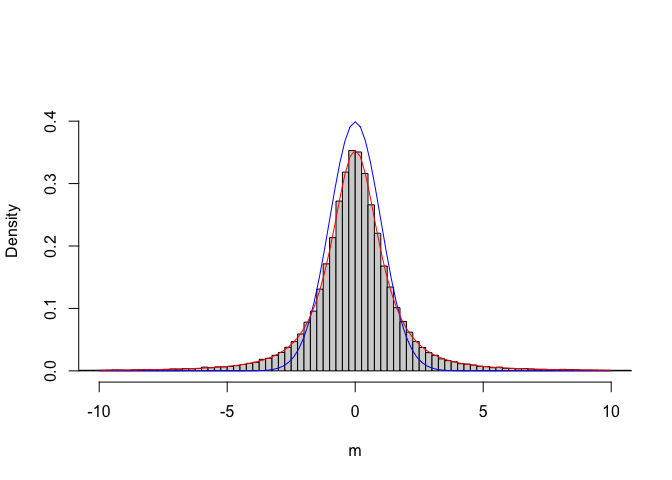
\includegraphics[width=0.85\linewidth]{_main_files/figure-latex/figName71-1} 

}

\caption{Empirical sampling distribution for the T statistic, compared to a standardised gaussian (blue line) and a Student's t distribution with 8 degree of freedom (red line)}\label{fig:figName71}
\end{figure}

We see that the empirical distribution is not exactly standardised gaussian, but it can be described by using another type of distribution, that is the Student's t distribution, with eight degrees of freedom (i.e.~the sum of the degrees of freedom for the two samples). Now that we know this, instead of making a time consuming Monte Carlo simulation, we can use the Student's t CDF to calculate the P-value, as shown in the box below.

\begin{Shaded}
\begin{Highlighting}[]
\FunctionTok{pt}\NormalTok{(Ti, }\AttributeTok{df=}\DecValTok{8}\NormalTok{) }\CommentTok{\# probability that T \textgreater{} 4.5217}
\DocumentationTok{\#\# [1] 0.0009727349}
\FunctionTok{pt}\NormalTok{(}\SpecialCharTok{{-}}\NormalTok{Ti, }\AttributeTok{df=}\DecValTok{8}\NormalTok{, }\AttributeTok{lower.tail =}\NormalTok{ F) }\CommentTok{\# probability that T \textless{} {-}4.5217}
\DocumentationTok{\#\# [1] 0.0009727349}
\DecValTok{2} \SpecialCharTok{*} \FunctionTok{pt}\NormalTok{(Ti, }\AttributeTok{df=}\DecValTok{8}\NormalTok{) }\CommentTok{\#P{-}value}
\DocumentationTok{\#\# [1] 0.00194547}
\end{Highlighting}
\end{Shaded}

We see that the P-value is very close to that obtained by using simulation.

\hypertarget{the-t-test-with-r}{%
\subsection{The t test with R}\label{the-t-test-with-r}}

What we have just described is known as the Student's t-test and it is often used to compare the means of two samples. The null hypothesis is that the two samples are drawn from the same populations and, therefore, their means are not significantly different. In practice, what we do is:

\begin{enumerate}
\def\labelenumi{\arabic{enumi}.}
\tightlist
\item
  Calculate the means and standard errors for the two samples
\item
  Calculate the difference between the means
\item
  Calculate the SED
\item
  Calculate the observed \(T\) value
\item
  Use the Student's t CDF to retrieve the probabilities \(P(t < -T)\) and \(P(t > T)\)
\item
  Reject the null hypothesis if the sum of the above probabilities is lower than 0.05.
\end{enumerate}

More simply, we can reach the same solution by using the \texttt{t.test()} function in R, as shown in the box below.

\begin{Shaded}
\begin{Highlighting}[]
\FunctionTok{t.test}\NormalTok{(A, P, }\AttributeTok{paired =}\NormalTok{ F, }\AttributeTok{var.equal =}\NormalTok{ T)}
\DocumentationTok{\#\# }
\DocumentationTok{\#\#  Two Sample t{-}test}
\DocumentationTok{\#\# }
\DocumentationTok{\#\# data:  A and P}
\DocumentationTok{\#\# t = {-}4.5217, df = 8, p{-}value = 0.001945}
\DocumentationTok{\#\# alternative hypothesis: true difference in means is not equal to 0}
\DocumentationTok{\#\# 95 percent confidence interval:}
\DocumentationTok{\#\#  {-}22.951742  {-}7.448258}
\DocumentationTok{\#\# sample estimates:}
\DocumentationTok{\#\# mean of x mean of y }
\DocumentationTok{\#\#      70.2      85.4}
\end{Highlighting}
\end{Shaded}

Perhaps, it is worth to discuss the meaning of the two arguments `paired' and `var.equal,' which were set, respectively, to FALSE and TRUE. In some cases two measures are taken on the same subject and we are interested in knowing whether there is a significant difference between the first and the second measure. For example, let's imagine that we have given a group of five cows a certain drug and we have measured some blood parameter before and after the treatment. We would have a dataset composed by ten values, but we would only have five subjects, which would make a big difference with respect to our previous example.

In such a condition we talk about a paired t-test, which is performed by setting the argument `paired' to TRUE, as shown in the box below.

\begin{Shaded}
\begin{Highlighting}[]
\FunctionTok{t.test}\NormalTok{(A, P, }\AttributeTok{paired =}\NormalTok{ T, }\AttributeTok{var.equal =}\NormalTok{ T)}
\DocumentationTok{\#\# }
\DocumentationTok{\#\#  Paired t{-}test}
\DocumentationTok{\#\# }
\DocumentationTok{\#\# data:  A and P}
\DocumentationTok{\#\# t = {-}22.915, df = 4, p{-}value = 2.149e{-}05}
\DocumentationTok{\#\# alternative hypothesis: true difference in means is not equal to 0}
\DocumentationTok{\#\# 95 percent confidence interval:}
\DocumentationTok{\#\#  {-}17.04169 {-}13.35831}
\DocumentationTok{\#\# sample estimates:}
\DocumentationTok{\#\# mean of the differences }
\DocumentationTok{\#\#                   {-}15.2}
\end{Highlighting}
\end{Shaded}

The calculations are totally different and, therefore, the significance is, as well, different. In particular, we consider the five pairwise differences, their mean and their standard error, as shown below:

\begin{Shaded}
\begin{Highlighting}[]
\NormalTok{diff }\OtherTok{\textless{}{-}} \FunctionTok{mean}\NormalTok{(A }\SpecialCharTok{{-}}\NormalTok{ P)}
\NormalTok{SED }\OtherTok{\textless{}{-}} \FunctionTok{sd}\NormalTok{(A }\SpecialCharTok{{-}}\NormalTok{ P)}\SpecialCharTok{/}\FunctionTok{sqrt}\NormalTok{(}\DecValTok{5}\NormalTok{) }
\NormalTok{diff}\SpecialCharTok{/}\NormalTok{SED}
\DocumentationTok{\#\# [1] {-}22.91486}
\end{Highlighting}
\end{Shaded}

One further difference is that, as we have five subjects instead of ten, we only have four degrees of freedom.

In relation to the argument `var.equal,' you have perhaps noted that we made our Monte Carlo simulation by drawing samples from one gaussian distribution. However, the two samples might come from two gaussian distributions with the same mean and different standard deviations, which would modify our sampling distribution for \(T\), so that our P-level would become invalid. We talk about \textbf{heteroscedasticity} when the populations, and therefore the two samples, have different standard deviations. Otherwise we talk about \textbf{homoscedasticity}.

If we have reasons to suppose that the two samples come from populations with different standard deviations, we should use a heteroscedastic t-test (better known as Welch test). We can set the `var.equal' argument to FALSE, as shown in the box below.

\begin{Shaded}
\begin{Highlighting}[]
\FunctionTok{t.test}\NormalTok{(A, P, }\AttributeTok{paired =}\NormalTok{ F, }\AttributeTok{var.equal =}\NormalTok{ F)}
\DocumentationTok{\#\# }
\DocumentationTok{\#\#  Welch Two Sample t{-}test}
\DocumentationTok{\#\# }
\DocumentationTok{\#\# data:  A and P}
\DocumentationTok{\#\# t = {-}4.5217, df = 7.7977, p{-}value = 0.002076}
\DocumentationTok{\#\# alternative hypothesis: true difference in means is not equal to 0}
\DocumentationTok{\#\# 95 percent confidence interval:}
\DocumentationTok{\#\#  {-}22.986884  {-}7.413116}
\DocumentationTok{\#\# sample estimates:}
\DocumentationTok{\#\# mean of x mean of y }
\DocumentationTok{\#\#      70.2      85.4}
\end{Highlighting}
\end{Shaded}

We see that the test is slightly less powerful (lower P-value), due to a reduced number of degrees of freedom, that is approximated by using the Satterthwaite formula:

\[DF_s \simeq \frac{ \left( s^2_1 + s^2_2 \right)^2 }{ \frac{(s^2_1)^2}{DF_1} + \frac{(s^2_2)^2}{DF_2} }\]

which reduces to:

\[DF_s = 2 \times DF\]

when the two samples are homoscedastic (\(s_1 = s_2\)).

in our example:

\begin{Shaded}
\begin{Highlighting}[]
\NormalTok{dfS }\OtherTok{\textless{}{-}}\NormalTok{ (}\FunctionTok{var}\NormalTok{(A) }\SpecialCharTok{+} \FunctionTok{var}\NormalTok{(P))}\SpecialCharTok{\^{}}\DecValTok{2} \SpecialCharTok{/} 
\NormalTok{  ((}\FunctionTok{var}\NormalTok{(A)}\SpecialCharTok{\^{}}\DecValTok{2}\NormalTok{)}\SpecialCharTok{/}\DecValTok{4} \SpecialCharTok{+}\NormalTok{ (}\FunctionTok{var}\NormalTok{(P)}\SpecialCharTok{\^{}}\DecValTok{2}\NormalTok{)}\SpecialCharTok{/}\DecValTok{4}\NormalTok{)}
\NormalTok{dfS}
\DocumentationTok{\#\# [1] 7.79772}
\end{Highlighting}
\end{Shaded}

How do we decide whether the two samples have the same standard deviation and thus we can use a homoscedastic t-test? In general, we use a heteroscedastic t-test whenever the standard deviation for one sample is twice or three times as much with respect to the other, although some statisticians suggest that we should better use a heteroscedastic t-test in all cases, in order to increase our protection level against wrong rejections.

\hypertarget{comparing-proportions-the-chi2-test}{%
\section{\texorpdfstring{Comparing proportions: the \(\chi^2\) test}{Comparing proportions: the \textbackslash chi\^{}2 test}}\label{comparing-proportions-the-chi2-test}}

The t-test is very useful, but we can only use it with quantitative variables. What if we have a nominal response, e.g.~death/alive, germinated/ungerminated? Let's imagine an experiment where we have sprayed two populations of insects with an insecticide, respectively with or without an adjuvant. From one population (with adjuvant), we get a random sample of 75 insects and record 56 deaths, while from the other population (without adjuvant) we get a random sample of 50 insects and record 48 deaths.

In this case the sample efficacies are \(p_1 = 56/75 = 0.747\) and \(p_2 = 0.96\), but we are not interested in the samples, but in the whole populations, from where we sampled our insects.

If we remember Chapter 3, we may recall that the results of such an experiment reduce to a contingency table, as shown in the box below:

\begin{Shaded}
\begin{Highlighting}[]
\NormalTok{counts }\OtherTok{\textless{}{-}} \FunctionTok{c}\NormalTok{(}\DecValTok{56}\NormalTok{, }\DecValTok{19}\NormalTok{, }\DecValTok{48}\NormalTok{, }\DecValTok{2}\NormalTok{)}
\NormalTok{tab }\OtherTok{\textless{}{-}} \FunctionTok{matrix}\NormalTok{(counts, }\DecValTok{2}\NormalTok{, }\DecValTok{2}\NormalTok{, }\AttributeTok{byrow =}\NormalTok{ T)}
\FunctionTok{row.names}\NormalTok{(tab) }\OtherTok{\textless{}{-}} \FunctionTok{c}\NormalTok{(}\StringTok{"I"}\NormalTok{, }\StringTok{"IA"}\NormalTok{)}
\FunctionTok{colnames}\NormalTok{(tab) }\OtherTok{\textless{}{-}} \FunctionTok{c}\NormalTok{(}\StringTok{"D"}\NormalTok{, }\StringTok{"A"}\NormalTok{)}
\NormalTok{tab }\OtherTok{\textless{}{-}} \FunctionTok{as.table}\NormalTok{(tab)}
\NormalTok{tab}
\DocumentationTok{\#\#     D  A}
\DocumentationTok{\#\# I  56 19}
\DocumentationTok{\#\# IA 48  2}
\end{Highlighting}
\end{Shaded}

For such a table, we already know how to calculate a \(\chi^2\), which measures the dependency among the two traits (insecticide treatment and deaths); the observed value, for our sample, is 9.768 (see below).

\begin{Shaded}
\begin{Highlighting}[]
\FunctionTok{summary}\NormalTok{(tab)}
\DocumentationTok{\#\# Number of cases in table: 125 }
\DocumentationTok{\#\# Number of factors: 2 }
\DocumentationTok{\#\# Test for independence of all factors:}
\DocumentationTok{\#\#  Chisq = 9.768, df = 1, p{-}value = 0.001776}
\end{Highlighting}
\end{Shaded}

Clearly, like any other sample based statistic, the value of \(\chi^2\) changes any time we repeat the sampling effort. Therefore, the null hypothesis is:

\[H_o :\pi_1  = \pi_2  = \pi\]

Please, note that we make a reference to the populations, not to the samples. If this is true, what is the sampling distribution for \(\chi^2\)? And, what is the probability of obtaining a value of 9.768, or higher?

Although it is possible to set up a Monte Carlo simulation to derive an empirical distribution, we will not do so, for the sake of brevity. We anticipate that the sampling distribution for \(\chi^2\) can be described by using the \(\chi^2\) density function, with the appropriate number of degrees of freedom (the minimum between the number of columns and the number of rows, minus 1). In our case, we have only one degree of freedom and we can use the cumulative \(\chi^2\) distribution function to derive the probability of obtaining a value of 9.768, or higher:

\begin{Shaded}
\begin{Highlighting}[]
\FunctionTok{pchisq}\NormalTok{(}\FloatTok{9.76801}\NormalTok{, }\DecValTok{1}\NormalTok{, }\AttributeTok{lower.tail=}\NormalTok{F)}
\DocumentationTok{\#\# [1] 0.001775746}
\end{Highlighting}
\end{Shaded}

The P-value is much lower than 0.05 and thus we can reject the null. We can get to the same result by using the \texttt{chisq.test()} function:

\begin{Shaded}
\begin{Highlighting}[]
\FunctionTok{chisq.test}\NormalTok{(tab, }\AttributeTok{correct =}\NormalTok{ F)}
\DocumentationTok{\#\# }
\DocumentationTok{\#\#  Pearson\textquotesingle{}s Chi{-}squared test}
\DocumentationTok{\#\# }
\DocumentationTok{\#\# data:  tab}
\DocumentationTok{\#\# X{-}squared = 9.768, df = 1, p{-}value = 0.001776}
\end{Highlighting}
\end{Shaded}

Please, note the argument `correct = F.' A chi-square test is appropriate only when the number of subjects is high enough, e.g.~higher than 30 subjects, or so. If not, we should improve our result by applying the so-called continuity correction, by using the argument `correct = T,' that is the default option in R.

\hypertarget{correct-interpretation-of-the-p-value}{%
\section{Correct interpretation of the P-value}\label{correct-interpretation-of-the-p-value}}

We use the P-value as the tool to decide whether we should accept or reject the null, i.e.~we use it as an heuristic tool, which was exactly Ronald Fisher's original intention. Later work by Jarzy Neyman and Egon Pearson, around 1930, gave the P-value a slightly different meaning, i.e.~the probability of wrongly rejecting the null (so-called type I error rate: false positive). However, we should interpret such a probability with reference to the sampling distribution, not with reference to a single experiment. It means that we can say that: \emph{if the null is true and we repeat the experiment an infinite number of times, we have less than 5\% probability of obtaining such a high T or \(\chi^2\) value}. On the other hand, we cannot legitimately conclude our experiment by saying that: \emph{there is less then 5\% probability that we have reached wrong conclusions}. Indeed, we do not (and will never) know whether we have reached correct conclusions in our specific experiment, while our `false-positive' probability is only valid on the long run.

\hypertarget{conclusions-3}{%
\section{Conclusions}\label{conclusions-3}}

The intrinsic uncertainty in all experimental data does not allow us to reach conclusions and make decisions with no risk of error. As our aim is to reject hypotheses, we protect ourself as much as possible against the possibility of wrong rejection. To this aim, we use the P-value for the null hypothesis: if this is lower than the predefined yardstick level (usually \(\alpha = 0.05\)) we reject the null and we can be confident that such an heuristic, in the long run, will result in less than 5\% of wrong rejections.

Before concluding, we should point out that we do not only run the risk of committing a false-positive error (type I error), we also run the risk of committing a false negative error (type II error), whenever we fail to reject a false null hypothesis. These two type of errors are nicely put in Figure \ref{fig:figName72}, that is commonly available in the web.

\begin{figure}

{\centering 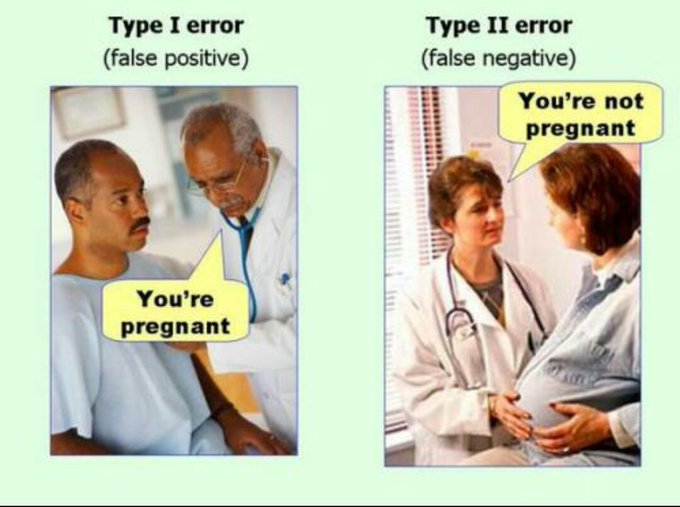
\includegraphics[width=0.85\linewidth]{_images/statisticalErrors} 

}

\caption{The two types of statistical errors}\label{fig:figName72}
\end{figure}

Please, also note that the two error types are interrelated and the highest the protection against the false-positive error, the highest the risk of committing a false negative error. In general, we should be always careful to decide which of the two errors might be more dangerous for our specific aim.

\begin{center}\rule{0.5\linewidth}{0.5pt}\end{center}

\hypertarget{further-readings-4}{%
\section{Further readings}\label{further-readings-4}}

\begin{enumerate}
\def\labelenumi{\arabic{enumi}.}
\tightlist
\item
  Hastie, T., Tibshirani, R., Friedman, J., 2009. The elements of statistical learning, Springer Series in Statistics. Springer Science + Business Media, California, USA.
\end{enumerate}

\hypertarget{one-way-anova-models}{%
\chapter{One-way ANOVA models}\label{one-way-anova-models}}

In Chapter 4 we have seen that the experimental observations can be described by way of models with both a deterministic and a stochastic component. With specific reference to the former component, we have already introduced an example of an ANOVA model, belonging to a very important class of linear models, where the response variable is quantitative, while the predictors are represented by one or several nominal explanatory factors. It is necessary to state that, strictly speaking, the term `ANOVA model' is slightly imprecise; indeed, ANOVA stands for ANalysis Of VAriance and it is a method for decomposing the variance of a group of observations, which was invented by Ronald Fisher, almost one century ago. However, the models we are discussing here are strongly connected to the Fisherian ANOVA, which motivates their name.

In this Chapter we will use a simple (but realistic) example to introduce the ANOVA models with only one predictor (one-way ANOVA models).

\hypertarget{comparing-herbicides-in-a-pot-experiment}{%
\section{Comparing herbicides in a pot-experiment}\label{comparing-herbicides-in-a-pot-experiment}}

We have designed a pot-experiment to compare weed control efficacy of two herbicides used alone and in mixture. A control was also added as a reference and, thus, the four treatments were:

\begin{enumerate}
\def\labelenumi{\arabic{enumi}.}
\tightlist
\item
  Metribuzin
\item
  Rimsulfuron
\item
  Metribuzin + rimsulfuron
\item
  Untreated control
\end{enumerate}

Sixteen uniform pots were prepared and sown with \emph{Solanum nigrum}; when the plants were at the stage of 4-true-leaves, the pots were randomly sprayed with the above herbicide solution, according to a completely randomised design with four replicates. Three weeks after the treatment, the plants in each pot were harvested and weighted: the lower the weight the higher the efficacy of herbicides.

The results of this experiment are reported in a `csv' file, that is available in a web repository. First of all, let's load the data into R.

\vspace{12pt}

\begin{Shaded}
\begin{Highlighting}[]
\NormalTok{repo }\OtherTok{\textless{}{-}} \StringTok{"https://www.casaonofri.it/\_datasets/"}
\NormalTok{file }\OtherTok{\textless{}{-}} \StringTok{"mixture.csv"}
\NormalTok{pathData }\OtherTok{\textless{}{-}} \FunctionTok{paste}\NormalTok{(repo, file, }\AttributeTok{sep =} \StringTok{""}\NormalTok{)}

\NormalTok{dataset }\OtherTok{\textless{}{-}} \FunctionTok{read.csv}\NormalTok{(pathData, }\AttributeTok{header =}\NormalTok{ T)}
\FunctionTok{head}\NormalTok{(dataset)}
\DocumentationTok{\#\#             Treat Weight}
\DocumentationTok{\#\# 1 Metribuzin\_\_348  15.20}
\DocumentationTok{\#\# 2 Metribuzin\_\_348   4.38}
\DocumentationTok{\#\# 3 Metribuzin\_\_348  10.32}
\DocumentationTok{\#\# 4 Metribuzin\_\_348   6.80}
\DocumentationTok{\#\# 5     Mixture\_378   6.14}
\DocumentationTok{\#\# 6     Mixture\_378   1.95}
\end{Highlighting}
\end{Shaded}

Please, note that the dataset is in a `tidy' format, with one row per observation and one column per variable. The first row contains the names of variables. i.e., `Treat,' representing the factor level and `Weight,' representing the response variable. While other data formats might be more suitable for visualisation, the `tidy' format is the base of every statistical analyses with most software tools and it can be easily transformed into other formats, whenever necessary (Wichkam, 2014).

\hypertarget{data-description}{%
\section{Data description}\label{data-description}}

The first step is the description of the observed data. In particular, we calculate:

\begin{enumerate}
\def\labelenumi{\arabic{enumi}.}
\tightlist
\item
  sample means for each treatment level
\item
  sample standard deviations for each treatment level
\end{enumerate}

To do so, we use the \texttt{tapply()} function, as shown in the box below and we also use the \texttt{data.frame()} function to create a data table for visualisation purposes.

\vspace{12pt}

\begin{Shaded}
\begin{Highlighting}[]
\NormalTok{treatMeans }\OtherTok{\textless{}{-}} \FunctionTok{tapply}\NormalTok{(dataset}\SpecialCharTok{$}\NormalTok{Weight, dataset}\SpecialCharTok{$}\NormalTok{Treat, mean)}
\NormalTok{SDs }\OtherTok{\textless{}{-}} \FunctionTok{tapply}\NormalTok{(dataset}\SpecialCharTok{$}\NormalTok{Weight, dataset}\SpecialCharTok{$}\NormalTok{Treat, sd)}
\NormalTok{descrit }\OtherTok{\textless{}{-}} \FunctionTok{data.frame}\NormalTok{(treatMeans, SDs)}
\NormalTok{descrit}
\DocumentationTok{\#\#                 treatMeans      SDs}
\DocumentationTok{\#\# Metribuzin\_\_348     9.1750 4.699089}
\DocumentationTok{\#\# Mixture\_378         5.1275 2.288557}
\DocumentationTok{\#\# Rimsulfuron\_30     16.8600 4.902353}
\DocumentationTok{\#\# Unweeded           26.7725 3.168673}
\end{Highlighting}
\end{Shaded}

What do we learn, from the above table of means? We learn that:

\begin{enumerate}
\def\labelenumi{\arabic{enumi}.}
\tightlist
\item
  the mixture is slightly more effective than the herbicides used alone;
\item
  the standard deviations are rather similar, for all treatments.
\end{enumerate}

Now, we ask ourselves: is there any significant difference between the efficacy of herbicides? If we look at the data, the answer is yes; indeed, the four means are different. However, we do not want to reach conclusions about our dataset; we want to reach general conclusions. We observed the four means \(m_1\), \(m_2\), \(m_3\) and \(m_4\), but we are interested in \(\mu_1\), \(\mu_2\), \(\mu_3\) and \(\mu_4\), i.e.~the means of the populations from where our samples were drawn. What are the populations, in this case? They consist of all possible pots that we could have treated with each herbicide, in our same environmental conditions.

\hypertarget{model-definition}{%
\section{Model definition}\label{model-definition}}

In order to answer the above question, we need to define a suitable model to describe our dataset. A possible candidate model is:

\[Y_i = \mu + \alpha_j + \varepsilon_i\]

This model postulates that each observation \(Y_i\) derives from the value \(\mu\) (so called intercept and common to all observations) plus the amount \(\alpha_j\), that depends on the treatment group \(j\), plus the stochastic effect \(\varepsilon_i\), which is specific to each observation and represents the experimental error. This stochastic element is regarded as gaussian distributed, with mean equal to 0 and standard deviation equal to \(\sigma\). In mathematical terms:

\[\varepsilon_i \sim N(0, \sigma)\]

The expected value for each observation, depending on the treatment group, is

\[\bar{Y_i} = \mu + \alpha_j = \mu_j\]

and corresponds to the group mean. In order to understand the biological meaning of \(\mu\) and \(\alpha\) values we need to go a little bit more into the mathematical detail.

\hypertarget{parameterisation}{%
\subsection{Parameterisation}\label{parameterisation}}

Let's consider the first observation \(Y_1 = 15.20\); we need to estimate three values (\(\mu\), \(\alpha_1\) and \(\varepsilon_1\)) which return 15.20, by summation. Clearly, there is an infinite number of such triplets and, therefore, the estimation problem is undetermined, unless we put constraints on some model parameters. There are several ways to put such constraints, corresponding to different \textbf{model parameterisations}; in the following section, we will list two of them: the treatment constraint and the sum-to-zero constraint.

\hypertarget{treatment-constraint}{%
\subsection{Treatment constraint}\label{treatment-constraint}}

A very common constraint is \(\alpha_1 = 0\). As the consequence:

\[\left\{ {\begin{array}{l}
\mu_1 = \mu + \alpha_1 = \mu + 0\\
\mu_2 = \mu + \alpha_2 \\
\mu_3 = \mu + \alpha_3 \\
\mu_4 = \mu + \alpha_4
\end{array}} \right.\]

With such a constraint, \(\mu\) is the mean for the first treatment level (in R, it is the first in alphabetical order), while \(\alpha_2\), \(\alpha_3\) and \(\alpha_4\) are the differences between, respectively, the second, third and fourth treatment level means, with respect to the first one.

In general, with this parameterisation, model parameters are means or differences between means.

\hypertarget{sum-to-zero-constraint}{%
\subsection{Sum-to-zero constraint}\label{sum-to-zero-constraint}}

Another possible constraint is \(\sum{\alpha_j} = 0\). If we take the previous equation and sum all members we get:

\[\mu_1 + \mu_2 + \mu_3 + \mu_4 = 4 \mu + \sum{\alpha_j}\]

Imposing the sum-to-zero constraint we get to:

\[\mu_1 + \mu_2 + \mu_3 + \mu_4 = 4 \mu\]

and then to:

\[\mu = \frac{\mu_1 + \mu_2 + \mu_3 + \mu_4}{4}\]

Therefore, with this parameterisation \(\mu\) is the overall mean, while the \(\alpha_j\) values represent the differences between each treatment mean and the overall mean (\textbf{treatment effects}). A very effective herbicide will have low negative \(\alpha\) values, while a bad herbicide will have high positive \(\alpha\) values.

In general, with this parameterisation, model parameters represent the overall mean and the effects of the different treatments.

The selection of constraints is up to the user, depending on the aims of the experiment. In this book, we will use the sum-to-zero constraint for our hand-calculations, as parameter estimates are easier to obtain and have a clearer biological meaning. In R, the treatment constraint is used by default, although the sum-to-zero constraint can be easily obtained, by using the appropriate coding. Independent on model parameterisation, the expected values, the residuals and all the other statistics are totally equal.

\hypertarget{basic-assumptions}{%
\section{Basic assumptions}\label{basic-assumptions}}

The ANOVA model above makes a number of \textbf{basic assumptions}:

\begin{enumerate}
\def\labelenumi{\arabic{enumi}.}
\tightlist
\item
  the effects are purely additive;
\item
  there are no other effects apart from the treatment and random noise. In particular, there are no components of systematic error;
\item
  errors are independently sampled from a gaussian distribution;
\item
  error variances are homogeneous, independent from the experimental treatments (indeed, we only have one \(\sigma\) value, common to all treatment groups)
\end{enumerate}

\textbf{We need to always make sure that the above assumptions are tenable, otherwise our model will be invalid, as well as all inferences therein}. We will discuss this aspect in the next chapter.

\hypertarget{fitting-anova-models-by-hand}{%
\section{Fitting ANOVA models by hand}\label{fitting-anova-models-by-hand}}

Model fitting is the process by which we take the general model defined above and use the data to find the most appropriate values for the unknown parameters. In general, linear models are fitted by using the least squares approach, i.e.~we look for the parameter values that minimise the squared difference between the observed data and model predictions. Nowadays, such minimisation is always carried out by using a computer, although we think that, once in life, fitting ANOVA models by hand may be very helpful, to understand the fundamental meaning of such a brilliant technique. In order to ease the process, we will not use the least squares method, but we will use the arithmetic means and the method of moments. Please, remember that this method is only appropriate when the data are balanced, i.e.~when the number of replicates is the same for all treatment groups.

\hypertarget{parameter-estimation}{%
\subsection{Parameter estimation}\label{parameter-estimation}}

According to the sum-to-zero constraint, we calculate the overall mean (m) as:

\vspace{12pt}

\begin{Shaded}
\begin{Highlighting}[]
\NormalTok{m }\OtherTok{\textless{}{-}} \FunctionTok{mean}\NormalTok{(dataset}\SpecialCharTok{$}\NormalTok{Weight)}
\NormalTok{mu }\OtherTok{\textless{}{-}}\NormalTok{ m}
\end{Highlighting}
\end{Shaded}

and our point estimate is \(\mu = m = 14.48375\). Next, we can estimate the \(\alpha\) effects by subtracting the overall mean from the group means:

\vspace{12pt}

\begin{Shaded}
\begin{Highlighting}[]
\NormalTok{alpha }\OtherTok{\textless{}{-}}\NormalTok{ treatMeans }\SpecialCharTok{{-}}\NormalTok{ mu}
\NormalTok{alpha}
\DocumentationTok{\#\# Metribuzin\_\_348     Mixture\_378  Rimsulfuron\_30 }
\DocumentationTok{\#\#        {-}5.30875        {-}9.35625         2.37625 }
\DocumentationTok{\#\#        Unweeded }
\DocumentationTok{\#\#        12.28875}
\end{Highlighting}
\end{Shaded}

Please, note that the last parameter \(\alpha_4\) was not `freely' selected, as it was implicitly constrained to be:

\[\alpha_4 = - \left( \alpha_1 + \alpha_2 + \alpha_3 \right)\]

Now, to proceed with our hand-calculations, we need to repeat each \(\alpha\) value four times, so that each original observation is matched to the correct \(\alpha\) value, depending on the treatment group (see later).

\vspace{12pt}

\begin{Shaded}
\begin{Highlighting}[]
\NormalTok{alpha }\OtherTok{\textless{}{-}} \FunctionTok{rep}\NormalTok{(alpha, }\AttributeTok{each =} \DecValTok{4}\NormalTok{)}
\end{Highlighting}
\end{Shaded}

\hypertarget{residuals}{%
\subsection{Residuals}\label{residuals}}

After deriving \(\mu\) and \(\alpha\) values, we can calculate the expected values by using the equation above and, lately, the residuals, as:

\[ \varepsilon_i = Y_i - \left( \mu - \alpha_j \right)\]

The results are shown in the following prospect:

\vspace{12pt}

\begin{Shaded}
\begin{Highlighting}[]
\NormalTok{Expected }\OtherTok{\textless{}{-}}\NormalTok{ mu }\SpecialCharTok{+}\NormalTok{ alpha}
\NormalTok{Residuals }\OtherTok{\textless{}{-}}\NormalTok{ dataset}\SpecialCharTok{$}\NormalTok{Weight }\SpecialCharTok{{-}}\NormalTok{ Expected}
\NormalTok{tab }\OtherTok{\textless{}{-}} \FunctionTok{data.frame}\NormalTok{(dataset}\SpecialCharTok{$}\NormalTok{Treat, dataset}\SpecialCharTok{$}\NormalTok{Weight, mu,}
\NormalTok{             alpha, Expected, Residuals)}
\FunctionTok{names}\NormalTok{(tab)[}\DecValTok{1}\NormalTok{] }\OtherTok{\textless{}{-}} \StringTok{"Herbicide"}
\FunctionTok{print}\NormalTok{(tab, }\AttributeTok{digits =} \DecValTok{3}\NormalTok{)}
\DocumentationTok{\#\#          Herbicide dataset.Weight   mu alpha Expected}
\DocumentationTok{\#\# 1  Metribuzin\_\_348          15.20 14.5 {-}5.31     9.18}
\DocumentationTok{\#\# 2  Metribuzin\_\_348           4.38 14.5 {-}5.31     9.18}
\DocumentationTok{\#\# 3  Metribuzin\_\_348          10.32 14.5 {-}5.31     9.18}
\DocumentationTok{\#\# 4  Metribuzin\_\_348           6.80 14.5 {-}5.31     9.18}
\DocumentationTok{\#\# 5      Mixture\_378           6.14 14.5 {-}9.36     5.13}
\DocumentationTok{\#\# 6      Mixture\_378           1.95 14.5 {-}9.36     5.13}
\DocumentationTok{\#\# 7      Mixture\_378           7.27 14.5 {-}9.36     5.13}
\DocumentationTok{\#\# 8      Mixture\_378           5.15 14.5 {-}9.36     5.13}
\DocumentationTok{\#\# 9   Rimsulfuron\_30          10.50 14.5  2.38    16.86}
\DocumentationTok{\#\# 10  Rimsulfuron\_30          20.70 14.5  2.38    16.86}
\DocumentationTok{\#\# 11  Rimsulfuron\_30          20.74 14.5  2.38    16.86}
\DocumentationTok{\#\# 12  Rimsulfuron\_30          15.50 14.5  2.38    16.86}
\DocumentationTok{\#\# 13        Unweeded          24.62 14.5 12.29    26.77}
\DocumentationTok{\#\# 14        Unweeded          30.94 14.5 12.29    26.77}
\DocumentationTok{\#\# 15        Unweeded          24.02 14.5 12.29    26.77}
\DocumentationTok{\#\# 16        Unweeded          27.51 14.5 12.29    26.77}
\DocumentationTok{\#\#    Residuals}
\DocumentationTok{\#\# 1     6.0250}
\DocumentationTok{\#\# 2    {-}4.7950}
\DocumentationTok{\#\# 3     1.1450}
\DocumentationTok{\#\# 4    {-}2.3750}
\DocumentationTok{\#\# 5     1.0125}
\DocumentationTok{\#\# 6    {-}3.1775}
\DocumentationTok{\#\# 7     2.1425}
\DocumentationTok{\#\# 8     0.0225}
\DocumentationTok{\#\# 9    {-}6.3600}
\DocumentationTok{\#\# 10    3.8400}
\DocumentationTok{\#\# 11    3.8800}
\DocumentationTok{\#\# 12   {-}1.3600}
\DocumentationTok{\#\# 13   {-}2.1525}
\DocumentationTok{\#\# 14    4.1675}
\DocumentationTok{\#\# 15   {-}2.7525}
\DocumentationTok{\#\# 16    0.7375}
\end{Highlighting}
\end{Shaded}

\hypertarget{standard-deviation-sigma}{%
\subsection{\texorpdfstring{Standard deviation \(\sigma\)}{Standard deviation \textbackslash sigma}}\label{standard-deviation-sigma}}

In order to get an estimate for \(\sigma\), we calculate the Residual Sum of Squares (RSS):

\vspace{12pt}

\begin{Shaded}
\begin{Highlighting}[]
\NormalTok{RSS }\OtherTok{\textless{}{-}} \FunctionTok{sum}\NormalTok{(Residuals}\SpecialCharTok{\^{}}\DecValTok{2}\NormalTok{)}
\NormalTok{RSS}
\DocumentationTok{\#\# [1] 184.1774}
\end{Highlighting}
\end{Shaded}

In order to obtain the residual variance, we need to divide the RSS by the appropriate number of Degrees of Freedom (DF); the question is: what is this number? We need to consider that the residuals represent the differences between each observed value and the group mean; therefore, those residuals must sum up to zero within all treatment groups, so that we have 16 residuals, but only three per group are `freely' selected, while the fourth one must be equal to the opposite of the sum of the other three. Hence, the number of degrees of freedom is \(3 \times 4 = 12\).

In more general terms, the number of degrees of freedom for the RSS is \(p (k -1)\), where \(p\) is the number of treatments and \(k\) is the number of replicates (assuming that this number is constant across treatments). The residual variance is:

\[MS_{e}  = \frac{184.178}{12} = 15.348\]

Consequently, our best point estimate for \(\sigma\) is:

\[sigma =  \sqrt{15.348} = 3.9177\]

Now, we can use our point estimates for model parameters to calculate point estimates for the group means (e.g.: \(\mu_1 = \mu + \alpha_1\)), which, in this instance, are equal to the arithmetic means, although this is not generally true. However, we know that point estimates are not sufficient to draw general conclusions and we need to provide the appropriate confidence intervals.

\hypertarget{sem-and-sed}{%
\subsection{SEM and SED}\label{sem-and-sed}}

The standard errors for the four means are easily obtained, by the usual rule (\(k\) is the number of replicates):

\[SEM = \frac{s}{ \sqrt{k}} =  \frac{3.918}{ \sqrt{4}}\]

You may have noted that, for all experiments, there are two ways to calculate standard errors for the group means:

\begin{enumerate}
\def\labelenumi{\arabic{enumi}.}
\tightlist
\item
  by taking the standard deviations for each treatment group, as shown in Chapter 3. With \(k\) treatments, this method results in \(k\) different standard errors;
\item
  by taking the pooled standard deviation estimate \(s\). In this case, we have only one common SEM value, for all group means.
\end{enumerate}

You may wonder which method is the best. Indeed, if the basic assumption of variance homogeneity is tenable, the second method is better, as the pooled SEM is estimated with higher precision, with respect to the SEs for each group mean (12 degrees of freedom, instead of 3).

The standard error for the difference between any possible pairs of means is:

\[SED = \sqrt{ MS_{1} + MS_{2} } = \sqrt{ 2 \cdot \frac{MS_e}{n} } =  \sqrt{2}  \cdot \frac{3.9177}{\sqrt{4}} = \sqrt{2} \cdot SEM\]

\hypertarget{variance-partitioning}{%
\subsection{Variance partitioning}\label{variance-partitioning}}

Fitting the above model is prodromic to the Fisherian ANalysis Of VAriance, i.e.~the real ANOVA technique. The aim is to partition the total variability of all observations into two components: the first one is due to treatment effects and the other one is due to all other effects of random nature.

In practice, we start our hand calculations from the total sum of squares (SS), that is the squared sum of residuals for each value against the overall mean (see Chapter 3):

\[\begin{array}{c}
SS = \left(24.62 - 14.48375\right)^2 + \left(30.94 - 14.48375\right)^2 + ... \\
... + \left(15.50 - 14.48375\right)^2 = 1273.706
\end{array}\]

Total deviance relates to the all the effects, both from known and unknown sources (treatment + random effects). With R:

\vspace{12pt}

\begin{Shaded}
\begin{Highlighting}[]
\NormalTok{SS }\OtherTok{\textless{}{-}} \FunctionTok{sum}\NormalTok{( (dataset}\SpecialCharTok{$}\NormalTok{Weight }\SpecialCharTok{{-}}\NormalTok{ mu)}\SpecialCharTok{\^{}}\DecValTok{2}\NormalTok{ )}
\end{Highlighting}
\end{Shaded}

Second, we can consider that the RSS represents the amount of data variability produced by random effects. Indeed, the variability of data within each treatment group cannot be due to treatment effects.

Finally, we can consider that variability produced by treatment effects is measured by the \(\alpha\) values and, therefore, the treatment sum of squares (TSS) is given by the sum of squared \(\alpha\) values:

\vspace{12pt}

\begin{Shaded}
\begin{Highlighting}[]
\NormalTok{TSS }\OtherTok{\textless{}{-}} \FunctionTok{sum}\NormalTok{(tab}\SpecialCharTok{$}\NormalTok{alpha}\SpecialCharTok{\^{}}\DecValTok{2}\NormalTok{)}
\NormalTok{TSS}
\DocumentationTok{\#\# [1] 1089.529}
\end{Highlighting}
\end{Shaded}

Please, note that the sum of the residual sum of squares (RSS) and the treatment sum of squares (TSS) is exactly equal to the total sum of squares:

\vspace{12pt}

\begin{Shaded}
\begin{Highlighting}[]
\NormalTok{TSS }\SpecialCharTok{+}\NormalTok{ RSS}
\DocumentationTok{\#\# [1] 1273.706}
\end{Highlighting}
\end{Shaded}

The partitioning of total variance shows that random variability is much lower than treatment variability, although we know that we cannot directly compare two deviances, when they are based on a different number of DFs (see Chapter 3).

Therefore, we calculate the corresponding variances: we have seen that the RSS has 12 degrees of freedom and the related variance is \(MS_e = 15.348\). The TSS has 3 degrees of freedom, that is the number of treatment levels minus one; the related variance is:

\[MS_t = \frac{1089.529}{3} = 363.1762\]

These two variances (treatment and residual) can be directly compared. Fisher, in 1920, proposed the following F-ratio:

\[F = \frac{MS_t}{MS_e} = \frac{363.18}{15.348} = 23.663\]

It shows that the variability imposed by the experimental treatment is more than 23 times higher than the variability due to random noise, which supports the idea that the treatment effect is significant. However, we need a formal statistical test to support such a statement.

\hypertarget{hypothesis-testing}{%
\subsection{Hypothesis testing}\label{hypothesis-testing}}

Let me recall a basic concept that has already appeared before and it is going to return rather often in this book (apologies for this). We have observed a set of 16 data, coming from a pot-experiment, but these data represent only a sample of an infinite number of replicated experiments that we could perform. Therefore, the observed F value is just an instance of an infinite number of possible F values, which define a sampling distribution. How does such sampling distribution look like?

In order to determine the sampling distribution for the F-ratio, we need to make some hypotheses. The null hypothesis is that the treatments have no effects and, thus:

\[H_0: \mu_1 = \mu_2 = \mu_3 = \mu_4\]

Analogously:

\[H_0: \alpha_1 = \alpha_2 = \alpha_3 = \alpha_4 = 0\]

In other words, if \(H_0\) were true, the four samples would be drawn from the same gaussian population. What would become of the F-ratio? We could see this by using Monte Carlo simulation, but, for the sake of simplicity, let's exploit literature information: the American mathematician George Snedecor demonstrated that, when the null is true, the sample based F-ratio is distributed according to the F-distribution (Fisher-Snedecor distribution). In more detail, Snedecor defined a family of F-distributions, whose elements are selected, depending on the number of degrees of freedom at the numerator and denominator. For our example (three degrees of freedom at the numerator and 12 at the denominator), the F distribution is shown in Figure \ref{fig:figNameF}. We see that the mode is between 0 and 1, while the expected value is around 1. We also see that values above 6 are very unlikely.

\begin{figure}

{\centering 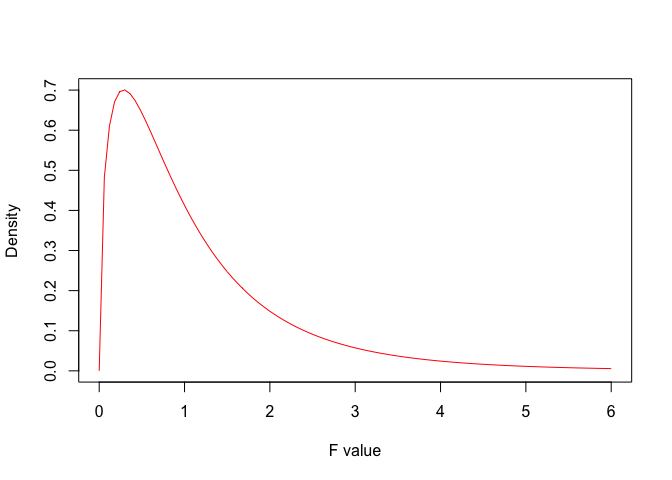
\includegraphics[width=0.9\linewidth]{_main_files/figure-latex/figNameF-1} 

}

\caption{Probabilty density function for F distribution with three and twelve degrees of freedom}\label{fig:figNameF}
\end{figure}

Now, we can use the cumulative distribution function in R to calculate the probability of obtaining values as high as 23.663 (the observed value) or higher:

\vspace{12pt}

\begin{Shaded}
\begin{Highlighting}[]
\FunctionTok{pf}\NormalTok{(}\FloatTok{23.663}\NormalTok{, }\DecValTok{3}\NormalTok{, }\DecValTok{12}\NormalTok{, }\AttributeTok{lower.tail =}\NormalTok{ F)}
\DocumentationTok{\#\# [1] 2.508789e{-}05}
\end{Highlighting}
\end{Shaded}

We can see that, if the hull is true and we repeat the experiment a very high humber of times, there is only one chance in 250,000 that we observe such a high F-value. As the consequence, we reject the null and accept the alternative, i.e.~there is at least one treatment level that produced a significant effect.

\hypertarget{fitting-anova-models-with-r}{%
\section{Fitting ANOVA models with R}\label{fitting-anova-models-with-r}}

Fitting models with R is very straightforward, by way of a very consistent platform for most types of models. For linear models, we use the \texttt{lm()} function, according to the following syntax:

\begin{verbatim}
mod <- lm(Weight ~ factor(Treat), data = dataset)
\end{verbatim}

The first argument is the equation we want to fit: on the left side, we specified the name of the response variable, the `tilde' means `is a function of and replaces the = sign and, on the right side, we specified the name of the factor variable. We did not specify the intercept and the stochastic term \(\varepsilon\), which are included by default. Please, also note that, prior to analysis, we transformed the 'Treat' variable into a factor, by using the \texttt{factor()} function. Such a transformation is not strictly necessary with character variables, but becomes fundamental with numeric variables, representing numbers and not classes.

\vspace{12pt}

\begin{Shaded}
\begin{Highlighting}[]
\NormalTok{dataset}\SpecialCharTok{$}\NormalTok{Treat }\OtherTok{\textless{}{-}} \FunctionTok{factor}\NormalTok{(dataset}\SpecialCharTok{$}\NormalTok{Treat)}
\NormalTok{mod }\OtherTok{\textless{}{-}} \FunctionTok{lm}\NormalTok{(Weight }\SpecialCharTok{\textasciitilde{}}\NormalTok{ Treat, }\AttributeTok{data =}\NormalTok{ dataset)}
\end{Highlighting}
\end{Shaded}

After fitting the model, results are written into the `mod' variable and can be read by using the appropriate extractor (\$ sign) or by using some of the available methods. For example, the \texttt{summary()} method returns parameter estimates, according to the treatment constraint, that is the default in R.

\vspace{12pt}
\scriptsize

\begin{Shaded}
\begin{Highlighting}[]
\FunctionTok{summary}\NormalTok{(mod)}
\DocumentationTok{\#\# }
\DocumentationTok{\#\# Call:}
\DocumentationTok{\#\# lm(formula = Weight \textasciitilde{} Treat, data = dataset)}
\DocumentationTok{\#\# }
\DocumentationTok{\#\# Residuals:}
\DocumentationTok{\#\#    Min     1Q Median     3Q    Max }
\DocumentationTok{\#\# {-}6.360 {-}2.469  0.380  2.567  6.025 }
\DocumentationTok{\#\# }
\DocumentationTok{\#\# Coefficients:}
\DocumentationTok{\#\#                     Estimate Std. Error t value Pr(\textgreater{}|t|)}
\DocumentationTok{\#\# (Intercept)            9.175      1.959   4.684 0.000529}
\DocumentationTok{\#\# TreatMixture\_378      {-}4.047      2.770  {-}1.461 0.169679}
\DocumentationTok{\#\# TreatRimsulfuron\_30    7.685      2.770   2.774 0.016832}
\DocumentationTok{\#\# TreatUnweeded         17.598      2.770   6.352 3.65e{-}05}
\DocumentationTok{\#\#                        }
\DocumentationTok{\#\# (Intercept)         ***}
\DocumentationTok{\#\# TreatMixture\_378       }
\DocumentationTok{\#\# TreatRimsulfuron\_30 *  }
\DocumentationTok{\#\# TreatUnweeded       ***}
\DocumentationTok{\#\# {-}{-}{-}}
\DocumentationTok{\#\# Signif. codes:  }
\DocumentationTok{\#\# 0 \textquotesingle{}***\textquotesingle{} 0.001 \textquotesingle{}**\textquotesingle{} 0.01 \textquotesingle{}*\textquotesingle{} 0.05 \textquotesingle{}.\textquotesingle{} 0.1 \textquotesingle{} \textquotesingle{} 1}
\DocumentationTok{\#\# }
\DocumentationTok{\#\# Residual standard error: 3.918 on 12 degrees of freedom}
\DocumentationTok{\#\# Multiple R{-}squared:  0.8554, Adjusted R{-}squared:  0.8193 }
\DocumentationTok{\#\# F{-}statistic: 23.66 on 3 and 12 DF,  p{-}value: 2.509e{-}05}
\end{Highlighting}
\end{Shaded}

\normalsize

For the sake of completeness, it might be useful to show that we can change the parameterisation, by setting the argument `contrasts' and passing a list of factors associated to the requested parameterisation (Treat = ``contr.sum,'' in this case). There are other methods to change the parameterisation, either globally (for the whole R session) or at the factor level; further information can be found in literature.

\vspace{12pt}

\begin{Shaded}
\begin{Highlighting}[]
\NormalTok{mod2 }\OtherTok{\textless{}{-}} \FunctionTok{lm}\NormalTok{(Weight }\SpecialCharTok{\textasciitilde{}}\NormalTok{ Treat, }\AttributeTok{data =}\NormalTok{ dataset,}
           \AttributeTok{contrasts =} \FunctionTok{list}\NormalTok{(}\AttributeTok{Treat =} \StringTok{"contr.sum"}\NormalTok{))}
\FunctionTok{summary}\NormalTok{(mod2)}\SpecialCharTok{$}\NormalTok{coef}
\DocumentationTok{\#\#             Estimate Std. Error   t value     Pr(\textgreater{}|t|)}
\DocumentationTok{\#\# (Intercept) 14.48375  0.9794169 14.788135 4.572468e{-}09}
\DocumentationTok{\#\# Treat1      {-}5.30875  1.6963999 {-}3.129421 8.701206e{-}03}
\DocumentationTok{\#\# Treat2      {-}9.35625  1.6963999 {-}5.515356 1.329420e{-}04}
\DocumentationTok{\#\# Treat3       2.37625  1.6963999  1.400761 1.866108e{-}01}
\end{Highlighting}
\end{Shaded}

Regardless of the parameterisation, fitted values and residuals can be obtained by using the \texttt{fitted()} and \texttt{residuals()} methods:

\vspace{12pt}

\begin{Shaded}
\begin{Highlighting}[]
\NormalTok{expected }\OtherTok{\textless{}{-}} \FunctionTok{fitted}\NormalTok{(mod)}
\NormalTok{epsilon }\OtherTok{\textless{}{-}} \FunctionTok{residuals}\NormalTok{(mod)}
\end{Highlighting}
\end{Shaded}

The residual deviance is:

\vspace{12pt}

\begin{Shaded}
\begin{Highlighting}[]
\FunctionTok{deviance}\NormalTok{(mod)}
\DocumentationTok{\#\# [1] 184.1774}
\end{Highlighting}
\end{Shaded}

while the residual standard deviation needs to be extracted from the slot `sigma,' from the output of the \texttt{summary()} method:

\vspace{12pt}

\begin{Shaded}
\begin{Highlighting}[]
\FunctionTok{summary}\NormalTok{(mod)}\SpecialCharTok{$}\NormalTok{sigma}
\DocumentationTok{\#\# [1] 3.917668}
\end{Highlighting}
\end{Shaded}

The ANOVA table is obtained by using the \texttt{anova()} method:

\vspace{12pt}

\begin{Shaded}
\begin{Highlighting}[]
\FunctionTok{anova}\NormalTok{(mod)}
\DocumentationTok{\#\# Analysis of Variance Table}
\DocumentationTok{\#\# }
\DocumentationTok{\#\# Response: Weight}
\DocumentationTok{\#\#           Df  Sum Sq Mean Sq F value    Pr(\textgreater{}F)    }
\DocumentationTok{\#\# Treat      3 1089.53  363.18  23.663 2.509e{-}05 ***}
\DocumentationTok{\#\# Residuals 12  184.18   15.35                      }
\DocumentationTok{\#\# {-}{-}{-}}
\DocumentationTok{\#\# Signif. codes:  }
\DocumentationTok{\#\# 0 \textquotesingle{}***\textquotesingle{} 0.001 \textquotesingle{}**\textquotesingle{} 0.01 \textquotesingle{}*\textquotesingle{} 0.05 \textquotesingle{}.\textquotesingle{} 0.1 \textquotesingle{} \textquotesingle{} 1}
\end{Highlighting}
\end{Shaded}

\hypertarget{expected-marginal-means}{%
\section{Expected marginal means}\label{expected-marginal-means}}

At the beginning of this chapter we have used the arithmetic means to describe the central tendency of each group. We have also seen that the sums \(\mu + \alpha_j\) return the group means, taking the name \textbf{Expected Marginal Means} (EMMs), which can also be used as measures of central tendency. When the experiment is balanced (same number of replicates for all groups), EMMs are equal to the arithmetic means, while, when the experiment is unbalanced, they differ and provide better estimators of population means.

In order to obtain expected marginal means with R, we need to install the add-in package `emmeans' (Lenth, 2016) and use the \texttt{emmeans()} function therein.

\vspace{12pt}

\begin{Shaded}
\begin{Highlighting}[]
\CommentTok{\# Install the package (only at the very first instance)}
\CommentTok{\# install.packages("emmeans") }
\FunctionTok{library}\NormalTok{(emmeans) }\CommentTok{\# Load the package}
\NormalTok{muj }\OtherTok{\textless{}{-}} \FunctionTok{emmeans}\NormalTok{(mod, }\SpecialCharTok{\textasciitilde{}}\NormalTok{Treat)}
\NormalTok{muj}
\DocumentationTok{\#\#  Treat           emmean   SE df lower.CL upper.CL}
\DocumentationTok{\#\#  Metribuzin\_\_348   9.18 1.96 12     4.91     13.4}
\DocumentationTok{\#\#  Mixture\_378       5.13 1.96 12     0.86      9.4}
\DocumentationTok{\#\#  Rimsulfuron\_30   16.86 1.96 12    12.59     21.1}
\DocumentationTok{\#\#  Unweeded         26.77 1.96 12    22.50     31.0}
\DocumentationTok{\#\# }
\DocumentationTok{\#\# Confidence level used: 0.95}
\end{Highlighting}
\end{Shaded}

\hypertarget{conclusions-4}{%
\section{Conclusions}\label{conclusions-4}}

Fitting ANOVA models is the subject of several chapters in this book. In practice, we are interested in assessing whether the effect of treatments produces a bigger data variability than all other unknown stochastic effects. We do so by using the F ratio that, under the null hypothesis, has a Fisher-Snedecor F distribution. If the observed F value and higher values are very unlikely to occur under the null, we reject it and conclude that the treatment effect was significant.

Finally, it is very important to point out that \textbf{all the above reasoning is only valid when the basic assumptions for linear models are met}. Therefore, it is always important to make the necessary inspections to ensure that there are no evident deviations, as we will see in the next chapter.

\begin{center}\rule{0.5\linewidth}{0.5pt}\end{center}

\hypertarget{further-readings-5}{%
\section{Further readings}\label{further-readings-5}}

\begin{enumerate}
\def\labelenumi{\arabic{enumi}.}
\tightlist
\item
  Faraway, J.J., 2002. Practical regression and Anova using R. \url{http://cran.r-project.org/doc/contrib/Faraway-PRA.pdf}.
\item
  Fisher, Ronald (1918). ``Studies in Crop Variation. I. An examination of the yield of dressed grain from Broadbalk'' (PDF). Journal of Agricultural Science. 11 (2): 107--135.
\item
  Kuehl, R. O., 2000. Design of experiments: statistical principles of research design and analysis. Duxbury Press (CHAPTER 2)
\item
  Lenth, R.V., 2016. Least-Squares Means: The R Package lsmeans. Journal of Statistical Software 69. \url{https://doi.org/10.18637/jss.v069.i01}
\item
  Wickham, H (2014) Tidy Data. J Stat Soft 59
\end{enumerate}

\hypertarget{checking-for-the-basic-assumptions}{%
\chapter{Checking for the basic assumptions}\label{checking-for-the-basic-assumptions}}

\ldots{}

\hypertarget{contrasts-and-multiple-comparison-testing}{%
\chapter{Contrasts and multiple comparison testing}\label{contrasts-and-multiple-comparison-testing}}

To be done \ldots{}

\hypertarget{multi-way-anova-models}{%
\chapter{Multi-way ANOVA models}\label{multi-way-anova-models}}

To be done \ldots{}

\hypertarget{multi-way-anova-models-with-interactions}{%
\chapter{Multi-way ANOVA models with interactions}\label{multi-way-anova-models-with-interactions}}

To be done \ldots{}

\hypertarget{plots-of-different-sizes}{%
\chapter{Plots of different sizes}\label{plots-of-different-sizes}}

To be done \ldots{}

\hypertarget{simple-linear-regression}{%
\chapter{Simple linear regression}\label{simple-linear-regression}}

To be done \ldots{}

\hypertarget{nonlinear-regression}{%
\chapter{Nonlinear regression}\label{nonlinear-regression}}

To be done \ldots{}

\hypertarget{exercises}{%
\chapter{Exercises}\label{exercises}}

\hypertarget{chapter-3}{%
\section{Chapter 3}\label{chapter-3}}

\hypertarget{exercise-1}{%
\subsection{Exercise 1}\label{exercise-1}}

A chemical analysis was performed in triplicate, with the following results: 125, 169 and 142 ng/g. Calculate mean, sum of squares, mean square, standard deviation and coefficient of variation.

\hypertarget{exercise-2}{%
\subsection{Exercise 2}\label{exercise-2}}

Download the Excel file `rimsulfuron.csv' from \url{https://www.casaonofri.it/_datasets/rimsulfuron.csv}. This is a dataset relating to a field experiment to compare 15 herbicides with 4 replicates. The response variables are maize yield and height. Describe the dataset and show the results on a barplot, including some measure of variability. Check whether yield correlates to height and comment on the results.

\hypertarget{exercise-3}{%
\subsection{Exercise 3}\label{exercise-3}}

Load the csv file `students.csv' from \url{https://www.casaonofri.it/_datasets/students.csv}. This dataset relates to a number of students, their votes in several undergraduate exams and information on high school. Determine whether (i) the average votes depend on the exam subject and (ii) the average votes depend on high school type.

\begin{center}\rule{0.5\linewidth}{0.5pt}\end{center}

\hypertarget{chapter-4}{%
\section{Chapter 4}\label{chapter-4}}

\hypertarget{exercise-1-1}{%
\subsection{Exercise 1}\label{exercise-1-1}}

A xenobiotic substance degrades in soil following a first-order kinetic, which is described by the following equation:

\[Y = 100 \, e^{-0.07 \, t}\]

where Y is the concentration at time \(t\). After spraying this substance in soil, what is the probability that 50 days later we observe a concentration below the toxicity threshold for mammalians (2 ng/g)? Please, consider that all the unknown sources of experimental error can be regarded as gaussian, with a coefficient of variability equal to 20\%.

\hypertarget{exercise-2-1}{%
\subsection{Exercise 2}\label{exercise-2-1}}

Crop yield is a function of its density, according to the following function:

\[ Y = 8 + 8 \, X - 0.07 \, X^2\]

Draw the graph and find the required density to obtain the highest yield (use a simple graphical method). What is the probability of obtaining a yield level between 2.5 and 3 t/ha, by using the optimal density? Consider that random variability is 12\%.

\hypertarget{exercise-3-1}{%
\subsection{Exercise 3}\label{exercise-3-1}}

The toxicity of a compound changes with the dose, according to the following expression:

\[ Y = \frac{1}{1 + exp\left\{ -2 \, \left[log(X) - log(15)\right] \right\}}\]

where \(Y\) is the proportion of dead animals and \(X\) is the dose. If we treat 150 animals with a dose of 35 g, what is the probability of finding more than 120 dead animals? The individual variability can be approximated by using a gaussian distribution, with a standard error equal to 10.

\hypertarget{exercise-4}{%
\subsection{Exercise 4}\label{exercise-4}}

Consider the sample C = {[}140 - 170 - 155{]}, which was drawn by a gaussian distribution. Calculate the probability of drawing an individual value from the same pupulation in the following intervals:

\begin{enumerate}
\def\labelenumi{\arabic{enumi}.}
\tightlist
\item
  higher than 170
\item
  lower than 140
\item
  within the range from 170 and 140
\end{enumerate}

\hypertarget{exercise-5}{%
\subsection{Exercise 5}\label{exercise-5}}

Consider a gaussian population with \(\mu\) = 23 and \(\sigma\) = 1. Calculate the probability of drawing three individuals with a mean

\begin{enumerate}
\def\labelenumi{\arabic{enumi}.}
\tightlist
\item
  higher than 25
\item
  lower than 21
\item
  between 21 and 25
\end{enumerate}

\begin{center}\rule{0.5\linewidth}{0.5pt}\end{center}

\hypertarget{chapter-5}{%
\section{Chapter 5}\label{chapter-5}}

\hypertarget{exercise-1-2}{%
\subsection{Exercise 1}\label{exercise-1-2}}

A chemical analysis was repeated three times, with the following results: 125, 169 and 142 ng/g. Calculate mean, deviance, variance, standard deviation, standard error and confidence intervals (P = 0.95 and P = 0.99).

\hypertarget{exercise-2-2}{%
\subsection{Exercise 2}\label{exercise-2-2}}

An experiment was carried out, comparing the yield of four wheat genotypes (in tons per hectar). The results are as follows:

\begin{tabular}{l|r|r|r|r}
\hline
Genotype & A & B & C & D\\
\hline
A & 5.22 & 6.02 & 5.08 & 6.67\\
\hline
B & 6.08 & 6.86 & 7.07 & 6.57\\
\hline
C & 4.42 & 5.63 & 4.49 & 4.89\\
\hline
D & 6.14 & 6.50 & 5.27 & 6.02\\
\hline
\end{tabular}

For each genotype, calculate the mean, deviance, variance, standard deviation, standard error and confidence interval (P = 0.95).

\hypertarget{exercise-3-2}{%
\subsection{Exercise 3}\label{exercise-3-2}}

We have measured the length of 30 maize seedlings, treated with selenium in water solution. The observed lengths are:

\begin{verbatim}
length <- c(2.07, 2.23, 2.04, 2.16, 2.12, 2.33, 2.21, 2.22, 2.29, 2.28, 
2.44, 2.04, 2.02, 1.49, 2.12, 2.38, 2.51, 2.27, 2.55, 2.44, 2.28, 
2.2, 2.03, 2.35, 2.34, 2.34, 1.99, 2.44, 2.44, 1.91)
\end{verbatim}

For the above sample, calculate the mean, deviance, variance, standard deviation, standard error and confidence interval (P = 0.95).

\hypertarget{exercise-4-1}{%
\subsection{Exercise 4}\label{exercise-4-1}}

A sample of 400 insects was sprayed with an insecticide and 136 individuals survived the treatment. Determine the efficacy of the insecticide, in terms of proportion of dead insects, together with 95\% confidence limits.

\begin{center}\rule{0.5\linewidth}{0.5pt}\end{center}

\hypertarget{chapter-6}{%
\section{Chapter 6}\label{chapter-6}}

\hypertarget{exercise-1-3}{%
\subsection{Exercise 1}\label{exercise-1-3}}

We have compared two herbicides for weed control in maize. With the first herbicide (A), we observed the following weed coverings: 9.3, 10.2, 9.7 \%. With the second herbicide, we observedd: 12.6, 12.3 e 12.5 \%. Are the means for the two herbicides significantly different (P \textless{} 0.05)?

\hypertarget{exercise-2-3}{%
\subsection{Exercise 2}\label{exercise-2-3}}

We have made an experiment to compare two fungicides A and B. The first fungicide was used to treat 200 fungi colonies and the number of surviving colonies was 180. B was used to treat 100 colonies and 50 of those survived. Is there a significant difference between the efficiacies of A and B (P \textless{} 0.05)?

\hypertarget{exercise-3-3}{%
\subsection{Exercise 3}\label{exercise-3-3}}

A plant pathologist studied the crop performances with (A) and without (NT) a fungicide treatment. The results are as follows:

\begin{longtable}[]{@{}cc@{}}
\toprule
A & NT \\
\midrule
\endhead
65 & 54 \\
71 & 51 \\
68 & 59 \\
\bottomrule
\end{longtable}

Was the treatment effect significant (P \textless{} 0.05)?

\hypertarget{exercise-4-2}{%
\subsection{Exercise 4}\label{exercise-4-2}}

In this year, an assay showed that 600 olive drupes out of 750 were attacked by \emph{Daucus olee}. In a close field, under the same environmental conditions, the count of attacked drupes was 120 on 750. Is the the observed difference statistically significant (P \textless{} 0.05) or is it just due to random fluctuation?

\hypertarget{exercise-5-1}{%
\subsection{Exercise 5}\label{exercise-5-1}}

In a hospital, blood cholesterol level was measured for eight patients, before and after a three months terapy. The observed values were:

\begin{longtable}[]{@{}ccl@{}}
\toprule
Patient & Before & After \\
\midrule
\endhead
1 & 167.3 & 126.7 \\
2 & 186.7 & 154.2 \\
3 & 105.0 & 107.9 \\
4 & 214.5 & 209.3 \\
5 & 148.5 & 138.5 \\
6 & 171.5 & 121.3 \\
7 & 161.5 & 112.4 \\
8 & 243.6 & 190.5 \\
\bottomrule
\end{longtable}

Can we say that this terapy is effective, or not?

\hypertarget{exercise-6}{%
\subsection{Exercise 6}\label{exercise-6}}

A plant breeder organised an experiment to compare three wheat genotypes, i.e.~GUERCINO, ARNOVA and BOLOGNA, according to a completely randomised design with 10 replicates. The observed yields are:

\begin{tabular}{c|c|c}
\hline
guercino & arnova & bologna\\
\hline
53.2 & 53.1 & 43.5\\
\hline
59.1 & 51.0 & 41.0\\
\hline
62.3 & 51.9 & 41.2\\
\hline
48.6 & 55.3 & 44.8\\
\hline
59.7 & 58.8 & 40.2\\
\hline
60.0 & 54.6 & 37.2\\
\hline
55.7 & 53.0 & 45.3\\
\hline
55.8 & 51.4 & 38.9\\
\hline
55.7 & 51.7 & 42.9\\
\hline
54.4 & 64.7 & 39.3\\
\hline
\end{tabular}

\begin{enumerate}
\def\labelenumi{\arabic{enumi}.}
\tightlist
\item
  Describe the three samples, by using the appropriate statistics of central tendency and spread
\item
  Infere the means of the pupulations from where the samples were drawn
\item
  For each of the three possible couples (GUERCINO vs ARNOVA, GUERCINO vs BOLOGNA and ARNOVA vs BOLOGNA), test the hypothesis that the two means are significantly different.
\end{enumerate}

\hypertarget{exercise-7}{%
\subsection{Exercise 7}\label{exercise-7}}

A botanist counted the number of germinated seeds for oilseed rape at two different temperatures (15 and 25°C). At 15°C, 358 germinations were counted out of 400 seeds. At 25°C, 286 germinations were counted out of 380 seeds.

\begin{enumerate}
\def\labelenumi{\arabic{enumi}.}
\tightlist
\item
  Describe the proportions of germination for the three samples
\item
  Infere the proportion of germinated seeds in the two populations, from where the samples of seeds were extracted (remember that the variance for a proportion is calculated as \(p \times (1- p)\).
\item
  Test the hypothesis that temperature had a significant effect on the germinability of oilseed rape seeds.
\end{enumerate}

\begin{center}\rule{0.5\linewidth}{0.5pt}\end{center}

\hypertarget{chapters-7-to-9}{%
\section{Chapters 7 to 9}\label{chapters-7-to-9}}

\hypertarget{exercise-1-4}{%
\subsection{Exercise 1}\label{exercise-1-4}}

An experiment was conducted with a completely randomised design to compare the yield of 5 wheat genotypes. The results (in bushels per acre) are as follows:

\begin{longtable}[]{@{}cccc@{}}
\toprule
Variety & 1 & 2 & 3 \\
\midrule
\endhead
A & 32.4 & 34.3 & 37.3 \\
B & 20.2 & 27.5 & 25.9 \\
C & 29.2 & 27.8 & 30.2 \\
D & 12.8 & 12.3 & 14.8 \\
E & 21.7 & 24.5 & 23.4 \\
\bottomrule
\end{longtable}

\begin{enumerate}
\def\labelenumi{\arabic{enumi}.}
\tightlist
\item
  Write the linear model for this study and explain the model components
\item
  Compute the ANOVA
\item
  Check for the basic assumptions
\item
  Compare the means
\item
  Present the results and comment on them
\end{enumerate}

The example is taken from: Le Clerg \emph{et al}. (1962)

\hypertarget{exercise-2-4}{%
\subsection{Exercise 2}\label{exercise-2-4}}

Cell cultures of tomato were grown by using three types of media, based on glucose, fructose and sucrose. The experiment was conducted with a completely randomised design with 5 replicates and a control was also added to the design. Cell growths are reported in the table below:

\begin{longtable}[]{@{}cccc@{}}
\toprule
Control & Glucose & Fructose & Sucrose \\
\midrule
\endhead
45 & 25 & 28 & 31 \\
39 & 28 & 31 & 37 \\
40 & 30 & 24 & 35 \\
45 & 29 & 28 & 33 \\
42 & 33 & 27 & 34 \\
\bottomrule
\end{longtable}

\begin{enumerate}
\def\labelenumi{\arabic{enumi}.}
\tightlist
\item
  Write the linear model for this study and explain the model components
\item
  Compute the ANOVA
\item
  Check for the basic assumptions
\item
  Compare the means
\item
  Present the results and comment on them
\end{enumerate}

\hypertarget{exercise-3-4}{%
\subsection{Exercise 3}\label{exercise-3-4}}

The failure time for a heating system was assessed, to discover the effect of the operating temperature. Four temperatures were tested with 6 replicates, according to a completely randomised design and the number of hours before failure were measured.
The results are as follows:

\begin{longtable}[]{@{}rr@{}}
\toprule
Temp. & Hours to failure \\
\midrule
\endhead
1520 & 1953 \\
1520 & 2135 \\
1520 & 2471 \\
1520 & 4727 \\
1520 & 6134 \\
1520 & 6314 \\
1620 & 1190 \\
1620 & 1286 \\
1620 & 1550 \\
1620 & 2125 \\
1620 & 2557 \\
1620 & 2845 \\
1660 & 651 \\
1660 & 837 \\
1660 & 848 \\
1660 & 1038 \\
1660 & 1361 \\
1660 & 1543 \\
1708 & 511 \\
1708 & 651 \\
1708 & 651 \\
1708 & 652 \\
1708 & 688 \\
1708 & 729 \\
\bottomrule
\end{longtable}

Please, note that these are the only possible values for temperature. Determine the best operating temperature, in order to delay failure.

\hypertarget{exercise-4-3}{%
\subsection{Exercise 4}\label{exercise-4-3}}

An entomologist counted the number of eggs laid from a lepidopter on three tobacco genotypes. 15 females were tested for each genotype and the results are as follows:

\begin{longtable}[]{@{}rrrr@{}}
\toprule
Female & Field & Resistant & USDA \\
\midrule
\endhead
1 & 211 & 0 & 448 \\
2 & 276 & 9 & 906 \\
3 & 415 & 143 & 28 \\
4 & 787 & 1 & 277 \\
5 & 18 & 26 & 634 \\
6 & 118 & 127 & 48 \\
7 & 1 & 161 & 369 \\
8 & 151 & 294 & 137 \\
9 & 0 & 0 & 29 \\
10 & 253 & 348 & 522 \\
11 & 61 & 0 & 319 \\
12 & 0 & 14 & 242 \\
13 & 275 & 21 & 261 \\
14 & 0 & 0 & 566 \\
15 & 153 & 218 & 734 \\
\bottomrule
\end{longtable}

Which is the most resistant genotype?

\begin{center}\rule{0.5\linewidth}{0.5pt}\end{center}

\hypertarget{chapter-10}{%
\section{Chapter 10}\label{chapter-10}}

\hypertarget{exercise-1-5}{%
\subsection{Exercise 1}\label{exercise-1-5}}

Data were collected about 5 types of irrigation on orange trees in Spain. The experiment was laid down as complete randomised blocks with 5 replicates and the results are as follows:

\begin{longtable}[]{@{}lccccc@{}}
\toprule
Method & 1 & 2 & 3 & 4 & 5 \\
\midrule
\endhead
Localised & 438 & 413 & 375 & 127 & 320 \\
Surface & 413 & 398 & 348 & 112 & 297 \\
Sprinkler & 346 & 334 & 281 & 43 & 231 \\
Sprinkler + localised & 335 & 321 & 267 & 33 & 219 \\
Submersion & 403 & 380 & 336 & 101 & 293 \\
\bottomrule
\end{longtable}

\begin{enumerate}
\def\labelenumi{\arabic{enumi}.}
\tightlist
\item
  Write the linear model for this study and explain the model components
\item
  Compute the ANOVA
\item
  Check for the basic assumptions
\item
  Compare the means
\item
  Present the results and comment on them
\end{enumerate}

\hypertarget{exercise-2-5}{%
\subsection{Exercise 2}\label{exercise-2-5}}

A fertilisation trial was conducted according to a RCBD with five replicates. One value is missing for the second treatment in the fifth block. The observed data are percentage contents in P\textsubscript{2} O\textsubscript{5} in leaf samples:

\begin{longtable}[]{@{}cccccc@{}}
\toprule
Treatment & 1 & 2 & 3 & 4 & 5 \\
\midrule
\endhead
Unfertilised & 5.6 & 6.1 & 5.3 & 5.9 & 9.4 \\
50 lb N & 7.3 & 6.0 & 7.7 & 7.7 & NA \\
100 lb N & 6.9 & 6.0 & 5.6 & 7.4 & 8.2 \\
50 lb N + 75 lb P2O5 & 10.8 & 11.2 & 8.8 & 10.4 & 12.9 \\
100 lb N + 75 lb P205 & 9.6 & 9.3 & 12 & 10.6 & 11.6 \\
\bottomrule
\end{longtable}

\begin{enumerate}
\def\labelenumi{\arabic{enumi}.}
\tightlist
\item
  Calculate arithmetic means
\item
  Calculate the ANOVA
\item
  Check for the basic assumptions
\item
  Calculate expected marginal means and compare to arithmetic means
\item
  The addition of P\textsubscript{2} O\textsubscript{5} is a convenient practice, in terms of agronomic effect?
\end{enumerate}

\hypertarget{exercise-3-5}{%
\subsection{Exercise 3}\label{exercise-3-5}}

A latin square experiment was planned to assess effect of four different fertilisers on lettuce yield. The observed data are as follows:

\begin{longtable}[]{@{}rccc@{}}
\toprule
Fertiliser & Row & Column & Yield \\
\midrule
\endhead
A & 1 & 1 & 104 \\
B & 1 & 2 & 114 \\
C & 1 & 3 & 90 \\
D & 1 & 4 & 140 \\
A & 2 & 4 & 134 \\
B & 2 & 3 & 130 \\
C & 2 & 1 & 144 \\
D & 2 & 2 & 174 \\
A & 3 & 3 & 146 \\
B & 3 & 4 & 142 \\
C & 3 & 2 & 152 \\
D & 3 & 1 & 156 \\
A & 4 & 2 & 147 \\
B & 4 & 1 & 160 \\
C & 4 & 4 & 160 \\
D & 4 & 3 & 163 \\
\bottomrule
\end{longtable}

\begin{enumerate}
\def\labelenumi{\arabic{enumi}.}
\tightlist
\item
  Write the linear model for this study and explain the model components
\item
  Compute the ANOVA
\item
  Check for the basic assumptions
\item
  Compare the means
\item
  Present the results and comment on them: what is the best fertiliser?
\end{enumerate}

\begin{center}\rule{0.5\linewidth}{0.5pt}\end{center}

\hypertarget{chapters-11-and-12}{%
\section{Chapters 11 and 12}\label{chapters-11-and-12}}

\hypertarget{exercise-1-6}{%
\subsection{Exercise 1}\label{exercise-1-6}}

A pot experiment was planned to evaluate the best timing for herbicide application against rhizome \emph{Sorghum halepense}. Five timings were compared (2-3, 4-5, 6-7 and 8-9 leaves), including a splitted treatment in two timings (3-4/8-9 leaves) and the untreated control. In order to understand whether the application is effective against plants coming from rhizomes of different sizes, a second factor was included in the experiment, i.e.~rhizome size (2, 4, six nodes). The design was a fully crossed two-way factorial, laid down as completely randomised with four replicates. The results (plant weights three weeks after the herbicide application) are as follows:

\begin{longtable}[]{@{}lcccccc@{}}
\toprule
Sizes ↓ / Timing → & 2-3 & 4-5 & 6-7 & 8-9 & 3-4/8-9 & Untreated \\
\midrule
\endhead
2-nodes & 34.03 & 0.10 & 30.91 & 33.21 & 2.89 & 41.63 \\
& 22.31 & 6.08 & 35.34 & 43.44 & 19.06 & 22.96 \\
& 21.70 & 3.73 & 24.23 & 44.06 & 0.10 & 52.14 \\
& 14.90 & 9.15 & 28.27 & 35.34 & 0.68 & 59.81 \\
4-nodes & 42.19 & 14.86 & 52.34 & 39.06 & 8.62 & 68.15 \\
& 51.06 & 36.03 & 43.17 & 61.59 & 0.05 & 42.75 \\
& 43.77 & 21.85 & 57.28 & 48.89 & 0.10 & 57.77 \\
& 31.74 & 8.71 & 29.71 & 49.14 & 9.65 & 44.85 \\
6-nodes & 20.84 & 11.37 & 55.00 & 41.77 & 9.80 & 43.20 \\
& 26.12 & 2.24 & 28.46 & 37.38 & 0.10 & 40.68 \\
& 35.24 & 14.17 & 21.81 & 39.55 & 1.42 & 34.11 \\
& 13.32 & 23.93 & 60.72 & 48.37 & 6.83 & 32.21 \\
\bottomrule
\end{longtable}

\begin{enumerate}
\def\labelenumi{\arabic{enumi}.}
\tightlist
\item
  Write the linear model for this study and explain the model components
\item
  Compute the ANOVA
\item
  Check for the basic assumptions
\item
  Calculate marginal means and cell means
\item
  Present the results and comment on them: what type of means should you report?
\end{enumerate}

\hypertarget{exercise-2-6}{%
\subsection{Exercise 2}\label{exercise-2-6}}

Six faba bean genotypes were tested in two sowing times, according to a plit-plot design in 4 complete blocks. Sowing times were randomised to main-plots within blocks and genotypes were randomised to sub-plots within main-plots and blocks. Results are:

\begin{longtable}[]{@{}lrcccc@{}}
\toprule
Sowing Time & Genotype & 1 & 2 & 3 & 4 \\
\midrule
\endhead
Autum & Chiaro & 4.36 & 4.00 & 4.23 & 3.83 \\
& Collameno & 3.01 & 3.32 & 3.27 & 3.40 \\
& Palombino & 3.85 & 3.85 & 3.68 & 3.98 \\
& Scuro & 4.97 & 3.98 & 4.39 & 4.14 \\
& Sicania & 4.38 & 4.01 & 3.94 & 2.99 \\
& Vesuvio & 3.94 & 4.47 & 3.93 & 4.21 \\
Spring & Chiaro & 2.76 & 2.64 & 2.25 & 2.38 \\
& Collameno & 2.50 & 1.79 & 1.57 & 1.77 \\
& Palombino & 2.24 & 2.21 & 2.50 & 2.05 \\
& Scuro & 3.45 & 2.94 & 3.12 & 2.69 \\
& Sicania & 3.24 & 3.60 & 3.16 & 3.08 \\
& Vesuvio & 2.34 & 2.44 & 1.71 & 2.00 \\
\bottomrule
\end{longtable}

\begin{enumerate}
\def\labelenumi{\arabic{enumi}.}
\tightlist
\item
  Write the linear model for this study and explain the model components
\item
  Compute the ANOVA
\item
  Check for the basic assumptions
\item
  Calculate marginal means and cell means
\item
  Present the results and comment on them: what type of means should you report?
\end{enumerate}

\hypertarget{exercise-3-6}{%
\subsection{Exercise 3}\label{exercise-3-6}}

Four crops were sown in soil 20 days after the application of three herbicide treatments, in order to evaluate possible carry-over effects of residuals. The untreated control was also added for comparison and the weight of plants was assessed four weeks after sowing. The experiment was laid down as strip-plot and, within each block, the herbicide were randomised to rows and crops to columns. The weight of plants is reported below:

\begin{longtable}[]{@{}lccccc@{}}
\toprule
Herbidicide & Block & sorghum & rape & soyabean & sunflower \\
\midrule
\endhead
Untreated & 1 & 180 & 157 & 199 & 201 \\
& 2 & 236 & 111 & 257 & 358 \\
& 3 & 287 & 217 & 346 & 435 \\
& 4 & 350 & 170 & 211 & 327 \\
Imazethapyr & 1 & 47 & 10 & 193 & 51 \\
& 2 & 43 & 1 & 113 & 4 \\
& 3 & 0 & 20 & 187 & 13 \\
& 4 & 3 & 21 & 122 & 15 \\
primisulfuron & 1 & 271 & 8 & 335 & 379 \\
& 2 & 182 & 0 & 201 & 201 \\
& 3 & 283 & 22 & 206 & 307 \\
& 4 & 147 & 24 & 240 & 337 \\
rimsulfuron & 1 & 403 & 238 & 226 & 290 \\
& 2 & 227 & 169 & 195 & 494 \\
& 3 & 400 & 364 & 257 & 397 \\
& 4 & 171 & 134 & 137 & 180 \\
\bottomrule
\end{longtable}

\begin{enumerate}
\def\labelenumi{\arabic{enumi}.}
\tightlist
\item
  Write the linear model for this study and explain the model components
\item
  Compute the ANOVA
\item
  Check for the basic assumptions
\item
  Calculate marginal means and cell means
\item
  Present the results and comment on them: what type of means should you report?
\end{enumerate}

\hypertarget{exercise-4-4}{%
\subsection{Exercise 4}\label{exercise-4-4}}

A field experiment was conducted to evaluate the effect of fertilisation timing (early, medium, late) on two genotypes. The experiment was designed as a randomised complete block design and the data represent the amount of absorbed nitrogen by the plant:

\begin{longtable}[]{@{}lcccc@{}}
\toprule
Genotype & Block & Early & Med & Late \\
\midrule
\endhead
A & 1 & 21.4 & 50.8 & 53.2 \\
& 2 & 11.3 & 42.7 & 44.8 \\
& 3 & 34.9 & 61.8 & 57.8 \\
B & 1 & 54.8 & 56.9 & 57.7 \\
& 2 & 47.9 & 46.8 & 54.0 \\
& 3 & 40.1 & 57.9 & 62.0 \\
\bottomrule
\end{longtable}

\begin{enumerate}
\def\labelenumi{\arabic{enumi}.}
\tightlist
\item
  Write the linear model for this study and explain the model components
\item
  Compute the ANOVA
\item
  Check for the basic assumptions
\item
  Calculate marginal means and cell means
\item
  Present the results and comment on them: what type of means should you report?
\end{enumerate}

\hypertarget{exercise-5-2}{%
\subsection{Exercise 5}\label{exercise-5-2}}

A study was carried out to evaluate the effect of washing temperature on the reduction of length for four types of fabric. Results are expressed as percentage reduction and the experiment was completely randomised, with two replicates:

\begin{longtable}[]{@{}ccccc@{}}
\toprule
Fabric & 210 °F & 215 °F & 220 °F & 225 °F \\
\midrule
\endhead
A & 1.8 & 2.0 & 4.6 & 7.5 \\
& 2.1 & 2.1 & 5.0 & 7.9 \\
B & 2.2 & 4.2 & 5.4 & 9.8 \\
& 2.4 & 4.0 & 5.6 & 9.2 \\
C & 2.8 & 4.4 & 8.7 & 13.2 \\
& 3.2 & 4.8 & 8.4 & 13.0 \\
D & 3.2 & 3.3 & 5.7 & 10.9 \\
& 3.6 & 3.5 & 5.8 & 11.1 \\
\bottomrule
\end{longtable}

Consider the temperature as a factor and:

\begin{enumerate}
\def\labelenumi{\arabic{enumi}.}
\tightlist
\item
  Write the linear model for this study and explain the model components
\item
  Compute the ANOVA
\item
  Check for the basic assumptions
\item
  Calculate marginal means and cell means
\item
  Present the results and comment on them: what type of means should you report?
\end{enumerate}

\hypertarget{exercise-6-1}{%
\subsection{Exercise 6}\label{exercise-6-1}}

A chemical process requires one alcohol and one base. A study is organised to evaluate the factorial combinations of three alcohols and two bases on the efficiency of the process, expressed as a percentage. The experiment is designd as completely randomised.

\begin{longtable}[]{@{}cccc@{}}
\toprule
Base & Alcohol 1 & Alcohol 2 & Alcohol 3 \\
\midrule
\endhead
A & 91.3 & 89.9 & 89.3 \\
& 88.1 & 89.5 & 87.6 \\
& 90.7 & 91.4 & 90.4 \\
& 91.4 & 88.3 & 90.3 \\
B & 87.3 & 89.4 & 92.3 \\
& 91.5 & 93.1 & 90.7 \\
& 91.5 & 88.3 & 90.6 \\
& 94.7 & 91.5 & 89.8 \\
\bottomrule
\end{longtable}

\begin{enumerate}
\def\labelenumi{\arabic{enumi}.}
\tightlist
\item
  Write the linear model for this study and explain the model components
\item
  Compute the ANOVA
\item
  Check for the basic assumptions
\item
  Calculate marginal means and cell means
\item
  Present the results and comment on them: what type of means should you report?
\end{enumerate}

\begin{center}\rule{0.5\linewidth}{0.5pt}\end{center}

\hypertarget{chapter-13}{%
\section{Chapter 13}\label{chapter-13}}

\hypertarget{exercise-1-7}{%
\subsection{Exercise 1}\label{exercise-1-7}}

A study was conducted to evaluate the effect of nitrogen fertilisation in lettuce. The experiment is completely randomised with 4 replicates and the yield results are as follows:

\begin{longtable}[]{@{}ccccc@{}}
\toprule
N level & B1 & B2 & B3 & B4 \\
\midrule
\endhead
0 & 124 & 114 & 109 & 124 \\
50 & 134 & 120 & 114 & 134 \\
100 & 146 & 132 & 122 & 146 \\
150 & 157 & 150 & 140 & 163 \\
200 & 163 & 156 & 156 & 171 \\
\bottomrule
\end{longtable}

\begin{enumerate}
\def\labelenumi{\arabic{enumi}.}
\tightlist
\item
  Write the linear model for this study and explain the model components
\item
  Estimate model parameters
\item
  Check for the basic assumptions
\item
  What yield might be obtained by using 120 kg N ha\textsuperscript{-1}?
\item
  Present the results and comment on them?
\end{enumerate}

\hypertarget{exercise-2-7}{%
\subsection{Exercise 2}\label{exercise-2-7}}

A study was conducted to evaluate the effect of increasing densities of a weed (\emph{Sinapis arvensis}) on sunflower yield. The experiment was completely randomised. Assuming that the yield response is linear, parameterise the model, check the goodness of fit and find the economical threshold level of weed density, considering that the yield worths 150 Euros per ton and the herbicide treatment costs 40 Euros per hectar. The observed results are:

\begin{longtable}[]{@{}crl@{}}
\toprule
density & Rep y & ield \\
\midrule
\endhead
0 & 1 & 36.63 \\
14 & 1 & 29.73 \\
19 & 1 & 32.12 \\
28 & 1 & 30.61 \\
32 & 1 & 27.7 \\
38 & 1 & 27.43 \\
54 & 1 & 24.79 \\
0 & 2 & 36.11 \\
14 & 2 & 34.72 \\
19 & 2 & 30.12 \\
28 & 2 & 30.8 \\
32 & 2 & 26.53 \\
38 & 2 & 27.6 \\
54 & 2 & 23.31 \\
0 & 3 & 38.35 \\
14 & 3 & 32.16 \\
19 & 3 & 31.72 \\
28 & 3 & 28.69 \\
32 & 3 & 25.88 \\
38 & 3 & 28.43 \\
54 & 3 & 30.26 \\
0 & 4 & 36.74 \\
14 & 4 & 32.566 \\
19 & 4 & 29.57 \\
28 & 4 & 33.663 \\
32 & 4 & 28.751 \\
38 & 4 & 27.114 \\
54 & 4 & 24.664 \\
\bottomrule
\end{longtable}

\begin{center}\rule{0.5\linewidth}{0.5pt}\end{center}

\hypertarget{chapter-14}{%
\section{Chapter 14}\label{chapter-14}}

\hypertarget{exercise-1-8}{%
\subsection{Exercise 1}\label{exercise-1-8}}

Two soil samples were treated with two herbicides and put in a climatic chamber at 20°C. Sub-samples were collected from both samples in different times and the concentration of herbicide residues was measured. The results are as follows:

\begin{longtable}[]{@{}ccc@{}}
\toprule
Time & Herbicide A & Herbicide B \\
\midrule
\endhead
0 & 100.00 & 100.00 \\
10 & 50.00 & 60.00 \\
20 & 25.00 & 40.00 \\
30 & 15.00 & 23.00 \\
40 & 7.00 & 19.00 \\
50 & 3.50 & 11.00 \\
60 & 2.00 & 5.10 \\
70 & 1.00 & 3.00 \\
\bottomrule
\end{longtable}

Assuming that the degradation follows an exponential decay trend, determine the half-life for both herbicides.

\hypertarget{exercise-2-8}{%
\subsection{Exercise 2}\label{exercise-2-8}}

A microbial population grows exponentially over time. Considering the following data, determine the relative rate of growth, by fitting the exponential growth model.

\begin{longtable}[]{@{}cc@{}}
\toprule
Time & Cells \\
\midrule
\endhead
0 & 2 \\
10 & 3 \\
20 & 5 \\
30 & 9 \\
40 & 17 \\
50 & 39 \\
60 & 94 \\
70 & 201 \\
\bottomrule
\end{longtable}

\hypertarget{exercise-3-7}{%
\subsection{Exercise 3}\label{exercise-3-7}}

An experiment was conducted to determine the absorption of nitrogen by roots of \emph{Lemna minor} in hydroponic colture. Results (N content) are the following:

\begin{longtable}[]{@{}cc@{}}
\toprule
Conc & Rate \\
\midrule
\endhead
2.86 & 14.58 \\
5.00 & 24.74 \\
7.52 & 31.34 \\
22.10 & 72.97 \\
27.77 & 77.50 \\
39.20 & 96.09 \\
45.48 & 96.97 \\
203.78 & 108.88 \\
\bottomrule
\end{longtable}

Use nonlinear least squares to estimate the parameters for the rectangular hyperbola (Michaelis-Menten model):

\[Y = \frac{a X} {b + X}\]

and make sure that model fit is good enough.

\hypertarget{exercise-4-5}{%
\subsection{Exercise 4}\label{exercise-4-5}}

An experiment was conducted to determine the yield of sunflower at increasing densities of a weed (\emph{Ammi majus}). Based on the following results, parameterise a rectangular hyperbola (\(Y = (a \, X)/(b + X)\) and test for possible lack of fit. The results are:

\begin{longtable}[]{@{}cr@{}}
\toprule
Weed density & Yield Loss (\%) \\
\midrule
\endhead
0 & 0 \\
23 & 17.9 \\
31 & 21.6 \\
39 & 26.9 \\
61 & 29.5 \\
\bottomrule
\end{longtable}

\hypertarget{exercise-5-3}{%
\subsection{Exercise 5}\label{exercise-5-3}}

An experiment was conducted in a pasture, to determine the effect of sampling area on the number of plant species (in general, the higher the sampling area and the higher the number of sampled species). The results are as follows:.

\begin{longtable}[]{@{}cr@{}}
\toprule
Area & N. of species \\
\midrule
\endhead
1 & 4 \\
2 & 5 \\
4 & 7 \\
8 & 8 \\
16 & 10 \\
32 & 14 \\
64 & 19 \\
128 & 22 \\
256 & 22 \\
\bottomrule
\end{longtable}

By using the above data, parameterise a power curve \(Y = a \, X^b\) and test for lack of fit.

\hypertarget{exercise-6-2}{%
\subsection{Exercise 6}\label{exercise-6-2}}

Crop growth can be often described by using a Gompertz model. The data below refer to an experiment were sugarbeet was grown either weed free, or weed infested; the weight of the crop per unit area was measured after six different numbers of Days After Emergence (DAE). The experiment was conducted by using a completely randomised design with three replicates and the results are reported below:

\begin{longtable}[]{@{}ccc@{}}
\toprule
DAE & Infested & Weed Free \\
\midrule
\endhead
21 & 0.06 & 0.07 \\
21 & 0.06 & 0.07 \\
21 & 0.11 & 0.07 \\
27 & 0.20 & 0.34 \\
27 & 0.20 & 0.40 \\
27 & 0.21 & 0.25 \\
38 & 2.13 & 2.32 \\
38 & 3.03 & 1.72 \\
38 & 1.27 & 1.22 \\
49 & 6.13 & 11.78 \\
49 & 5.76 & 13.62 \\
49 & 7.78 & 12.15 \\
65 & 17.05 & 33.11 \\
65 & 22.48 & 24.96 \\
65 & 12.66 & 34.66 \\
186 & 21.51 & 38.83 \\
186 & 26.26 & 27.84 \\
186 & 27.68 & 37.72 \\
\bottomrule
\end{longtable}

Parameterise two Gompertz growth models (one for the weed-free crop and one for the infested crop) and evalaute which of the parameters are most influenced by the competition. The Gompertz growth model is:

\[Y = d \cdot exp\left\{- exp \left[ - b (X - e)\right] \right\}\]

\hypertarget{exercise-7-1}{%
\subsection{Exercise 7}\label{exercise-7-1}}

Plants of \emph{Tripleuspermum inodorum} in pots were treated with a sulphonylurea herbicide (tribenuron-methyl) at increasing rates. Three weeks after the treatment the weight per pot was recorded, with the following results:

\begin{longtable}[]{@{}cc@{}}
\toprule
Dose (g a.i. ha\(^{-1}\)) & Fresh weight (g pot \(^{-1}\)) \\
\midrule
\endhead
0 & 115.83 \\
0 & 102.90 \\
0 & 114.35 \\
0.25 & 91.60 \\
0.25 & 103.23 \\
0.25 & 133.97 \\
0.5 & 98.66 \\
0.5 & 92.51 \\
0.5 & 124.19 \\
1 & 93.92 \\
1 & 49.21 \\
1 & 49.24 \\
2 & 21.85 \\
2 & 23.77 \\
2 & 22.46 \\
\bottomrule
\end{longtable}

Assuming that the dose-response relationship can be described by using the following log-logistic model:

\[Y = c + \frac{d - c}{1 + exp \left\{ - b \left[ log (X) - log (e) \right] \right\}}\]

Parameterise the model and evaluate the goodnes of fit.

\hypertarget{appendix-a-very-gentle-introduction-to-r}{%
\chapter{APPENDIX: A very gentle introduction to R}\label{appendix-a-very-gentle-introduction-to-r}}

\hypertarget{what-is-r}{%
\section{What is R?}\label{what-is-r}}

R is a statistical software; it is open source and it works under a freeware GNU licence. It is very powerful, but it has no graphical interface and, thus, we need to write a few lines of cod, which is something we may not be used to do.

\hypertarget{installing-r-and-moving-the-first-steps}{%
\section{Installing R and moving the first steps}\label{installing-r-and-moving-the-first-steps}}

In order to get started, please, follow these basic steps:

\begin{enumerate}
\def\labelenumi{\arabic{enumi}.}
\tightlist
\item
  Install R from: \url{https://cran.r-project.org}. Follow the link to CRAN (uppermost right side), select one of the available mirrors (you can simply select the first link on top), select your Operating System (OS) and download the base version. Install it by using all default options.
\item
  Install RStudio from: \url{https://rstudio.com/products/rstudio/}. Select RStudio Desktop version, open source edition and download. Install it by using all default options.
\item
  Launch RStudio.
\end{enumerate}

You will see that RStudio consists of four panes, even hough, at the beginning, we will only use two of them, named: (1) SOURCE and (2) CONSOLE. The basic principle is to write code in the SOURCE pane and send it to the CONSOLE pane, by hitting `ctrl-R' or `ctrl-Return' (`cmd-Return' in Mac OSx). The SOURCE pane is a text editor and we can save script files, by using the `.R' extension. The CONSOLE pane is where the code is processed, to return the results.

Before we start, there are a few important suggestions that we should keep into consideration, in order to save a few headackes:

\begin{enumerate}
\def\labelenumi{\arabic{enumi}.}
\tightlist
\item
  unlike most programs in WINDOWS, R is case-sensitive and, e.g., `A' is not the same as `a.' Please, note that most errors in R are due to small typos, which may take very long to be spotted!
\item
  Code written in the SOURCE pane \textbf{MUST BE} sent to the console pane, otherwise it is not executed. It's like writing a WhatsApp message: our mate cannot read our message until we send it away to him!
\item
  Spaces can be used to write clearer code and they are usually allowed, except within variable names, function names and some operators composed by more than one character.
\item
  It is useful to comment the code, so that, in future times, we can remember what we intended to do, when we wrote that code. Every line preceded by a hash symbol (\#) is not executed and it is regarded as a comment.
\end{enumerate}

\hypertarget{assignments}{%
\section{Assignments}\label{assignments}}

In R, we work with objects, that must be assigned a name, so that they can be stored in memory and easily recalled. The name is a \textbf{variable} and it is assigned by the assignment operator `\textless-' (Less-then sign + dash sign). For example, the following code assigns the value of 3 to the `y' variable. The content of a variable can be visualised by simply writing its names and sending it to the console.

\begin{Shaded}
\begin{Highlighting}[]
\NormalTok{y  }\OtherTok{\textless{}{-}}  \DecValTok{3}
\NormalTok{y}
\DocumentationTok{\#\# [1] 3}
\end{Highlighting}
\end{Shaded}

\hypertarget{data-types-and-data-objects}{%
\section{Data types and data objects}\label{data-types-and-data-objects}}

In R, as in most programming languages, we have different data types that can be assigned to a variable:

\begin{enumerate}
\def\labelenumi{\arabic{enumi}.}
\tightlist
\item
  numeric (real numbers)
\item
  integer (natural numbers)
\item
  character (use quotation marks: ``andrea'' or ``martina'')
\item
  factor
\item
  logic (boolean): TRUE or FALSE
\end{enumerate}

Depending on their type, data can be stored in specific objects. The most important object is the \textbf{vector}, that is a uni-dimensional array, storing data of the same type (either numeric, or integer, or logic\ldots{} you can't mix!). For example, the following box shows a vector of character strings and a vector of numeric values: we see that the vector is created by the \texttt{c()} function and the elements are separated by commas.

\begin{Shaded}
\begin{Highlighting}[]
\NormalTok{sentence }\OtherTok{\textless{}{-}} \FunctionTok{c}\NormalTok{(}\StringTok{"this"}\NormalTok{, }\StringTok{"is"}\NormalTok{, }\StringTok{"an"}\NormalTok{, }\StringTok{"array"}\NormalTok{, }\StringTok{"of"}\NormalTok{, }\StringTok{"characters"}\NormalTok{)}
\NormalTok{x }\OtherTok{\textless{}{-}} \FunctionTok{c}\NormalTok{(}\DecValTok{12}\NormalTok{, }\DecValTok{13}\NormalTok{, }\DecValTok{14}\NormalTok{)}
\end{Highlighting}
\end{Shaded}

The factor vector is different from a character vector, as it is used to store character values belonging to a predefined set of levels; the experimental treatment variables (experimental factors, as we called them in Chapter 2) are usually stored as R factors. The code below shows a character vector that is transformed into a factor, by using the \texttt{factor()} function.

\begin{Shaded}
\begin{Highlighting}[]
\NormalTok{treat  }\OtherTok{\textless{}{-}}  \FunctionTok{c}\NormalTok{(}\StringTok{"A"}\NormalTok{, }\StringTok{"A"}\NormalTok{, }\StringTok{"B"}\NormalTok{, }\StringTok{"B"}\NormalTok{, }\StringTok{"C"}\NormalTok{, }\StringTok{"C"}\NormalTok{)}
\NormalTok{treat}
\DocumentationTok{\#\# [1] "A" "A" "B" "B" "C" "C"}
\FunctionTok{factor}\NormalTok{(treat)}
\DocumentationTok{\#\# [1] A A B B C C}
\DocumentationTok{\#\# Levels: A B C}
\end{Highlighting}
\end{Shaded}

By now, we have already used a couple of functions ad we have noted that they are characterised by a name followed by a pair of round brackets (e.g., \texttt{c()} or \texttt{factor()}). The arguments go inside the brackets, but we will give more detail later on.

\hypertarget{matrices}{%
\section{Matrices}\label{matrices}}

Vectors are uni-dimensional arrays, while matrices are bi-dimensional arrays, with rows and columns. The matrix object can be used to store only data of the same type (like a vector) and it is created by using the \texttt{matrix()} function. The first argument to this function is a vector of values, the second argument is the number of rows and the third one is the number of columns. The fourth argument is logical and it specifies whether the matrix is to be populated by row (`byrow = TRUE') or by column (`byrow = FALSE').

\begin{Shaded}
\begin{Highlighting}[]
\NormalTok{z  }\OtherTok{\textless{}{-}}  \FunctionTok{matrix}\NormalTok{(}\FunctionTok{c}\NormalTok{(}\DecValTok{1}\NormalTok{, }\DecValTok{2}\NormalTok{, }\DecValTok{3}\NormalTok{, }\DecValTok{4}\NormalTok{, }\DecValTok{5}\NormalTok{, }\DecValTok{6}\NormalTok{, }\DecValTok{7}\NormalTok{, }\DecValTok{8}\NormalTok{),}
              \DecValTok{2}\NormalTok{, }\DecValTok{4}\NormalTok{, }\AttributeTok{byrow=}\ConstantTok{TRUE}\NormalTok{)}
\NormalTok{z}
\DocumentationTok{\#\#      [,1] [,2] [,3] [,4]}
\DocumentationTok{\#\# [1,]    1    2    3    4}
\DocumentationTok{\#\# [2,]    5    6    7    8}
\end{Highlighting}
\end{Shaded}

\hypertarget{dataframes}{%
\section{Dataframes}\label{dataframes}}

The dataframe is also a table (like a matrix), but columns can contain data of different types. It is the most common way to store the experimental data and it should be orginised in a `tidy' way: with one experimental unit per row and all the traits of each unit in different columns. In the box below we create three vectors and combine them in a dataframe.

\scriptsize

\begin{Shaded}
\begin{Highlighting}[]
\NormalTok{plot  }\OtherTok{\textless{}{-}}  \FunctionTok{c}\NormalTok{(}\DecValTok{1}\NormalTok{, }\DecValTok{2}\NormalTok{, }\DecValTok{3}\NormalTok{, }\DecValTok{4}\NormalTok{, }\DecValTok{5}\NormalTok{, }\DecValTok{6}\NormalTok{)}
\NormalTok{treat  }\OtherTok{\textless{}{-}}  \FunctionTok{factor}\NormalTok{(}\FunctionTok{c}\NormalTok{(}\StringTok{"A"}\NormalTok{, }\StringTok{"A"}\NormalTok{, }\StringTok{"B"}\NormalTok{, }\StringTok{"B"}\NormalTok{, }\StringTok{"C"}\NormalTok{, }\StringTok{"C"}\NormalTok{))}
\NormalTok{yield  }\OtherTok{\textless{}{-}}  \FunctionTok{c}\NormalTok{(}\DecValTok{12}\NormalTok{, }\DecValTok{15}\NormalTok{, }\DecValTok{16}\NormalTok{, }\DecValTok{13}\NormalTok{, }\DecValTok{11}\NormalTok{, }\DecValTok{19}\NormalTok{)}
\NormalTok{dataset  }\OtherTok{\textless{}{-}}  \FunctionTok{data.frame}\NormalTok{(}\StringTok{"Plot"} \OtherTok{=}\NormalTok{ plot,}
  \StringTok{"Treatment"} \OtherTok{=}\NormalTok{ treat, }\StringTok{"Yield"} \OtherTok{=}\NormalTok{ yield)}
\NormalTok{dataset}
\DocumentationTok{\#\#   Plot Treatment Yield}
\DocumentationTok{\#\# 1    1         A    12}
\DocumentationTok{\#\# 2    2         A    15}
\DocumentationTok{\#\# 3    3         B    16}
\DocumentationTok{\#\# 4    4         B    13}
\DocumentationTok{\#\# 5    5         C    11}
\DocumentationTok{\#\# 6    6         C    19}
\end{Highlighting}
\end{Shaded}

\normalsize

\hypertarget{working-with-objects}{%
\section{Working with objects}\label{working-with-objects}}

If we have created a number of objects and stored them in memory, we might be interested in viewing them or accessing some of their elements. Objects can be simply viewed by using their name, as shown below.

\begin{Shaded}
\begin{Highlighting}[]
\NormalTok{z}
\DocumentationTok{\#\#      [,1] [,2] [,3] [,4]}
\DocumentationTok{\#\# [1,]    1    2    3    4}
\DocumentationTok{\#\# [2,]    5    6    7    8}
\end{Highlighting}
\end{Shaded}

With objects containing more than one value (vectors, matrices or dataframes) we can use indexing to retreive an element in a specific position. Indexing is performed by using square brackets, containing the index or a list of indices, for multi-dimensional objects.

\begin{Shaded}
\begin{Highlighting}[]
\NormalTok{x[}\DecValTok{1}\NormalTok{] }\CommentTok{\# First element in a vector}
\DocumentationTok{\#\# [1] 12}
\NormalTok{z[}\DecValTok{1}\NormalTok{, }\DecValTok{3}\NormalTok{] }\CommentTok{\# Element in first row and third column, in a dataframe or matrix}
\DocumentationTok{\#\# [1] 3}
\NormalTok{dataset[ ,}\DecValTok{1}\NormalTok{] }\CommentTok{\# First Column}
\DocumentationTok{\#\# [1] 1 2 3 4 5 6}
\NormalTok{dataset[}\DecValTok{1}\NormalTok{, ] }\CommentTok{\# First Row}
\DocumentationTok{\#\#   Plot Treatment Yield}
\DocumentationTok{\#\# 1    1         A    12}
\end{Highlighting}
\end{Shaded}

Column vectors in dataframes can also be accessed by using their name and the `dollar' sign, as shown below.

\begin{Shaded}
\begin{Highlighting}[]
\NormalTok{dataset}\SpecialCharTok{$}\NormalTok{Plot}
\DocumentationTok{\#\# [1] 1 2 3 4 5 6}
\end{Highlighting}
\end{Shaded}

It is also useful to ask for infos about objects, which can be done by using two functions:

\begin{enumerate}
\def\labelenumi{\arabic{enumi}.}
\tightlist
\item
  \texttt{str()}: tells us the structure of an object
\item
  \texttt{summary()} - summarizes the main traits of an object
\end{enumerate}

\begin{Shaded}
\begin{Highlighting}[]
\FunctionTok{str}\NormalTok{(dataset)}
\DocumentationTok{\#\# \textquotesingle{}data.frame\textquotesingle{}:    6 obs. of  3 variables:}
\DocumentationTok{\#\#  $ Plot     : num  1 2 3 4 5 6}
\DocumentationTok{\#\#  $ Treatment: Factor w/ 3 levels "A","B","C": 1 1 2 2 3 3}
\DocumentationTok{\#\#  $ Yield    : num  12 15 16 13 11 19}
\FunctionTok{summary}\NormalTok{(dataset)}
\DocumentationTok{\#\#       Plot      Treatment     Yield      }
\DocumentationTok{\#\#  Min.   :1.00   A:2       Min.   :11.00  }
\DocumentationTok{\#\#  1st Qu.:2.25   B:2       1st Qu.:12.25  }
\DocumentationTok{\#\#  Median :3.50   C:2       Median :14.00  }
\DocumentationTok{\#\#  Mean   :3.50             Mean   :14.33  }
\DocumentationTok{\#\#  3rd Qu.:4.75             3rd Qu.:15.75  }
\DocumentationTok{\#\#  Max.   :6.00             Max.   :19.00}
\end{Highlighting}
\end{Shaded}

\hypertarget{expressions-functions-and-arguments}{%
\section{Expressions, functions and arguments}\label{expressions-functions-and-arguments}}

Expressions can be used to return results or store them in new variables.

\begin{Shaded}
\begin{Highlighting}[]
\DecValTok{2} \SpecialCharTok{*}\NormalTok{ y}
\DocumentationTok{\#\# [1] 6}
\NormalTok{f  }\OtherTok{\textless{}{-}}  \DecValTok{2} \SpecialCharTok{*}\NormalTok{ y}
\NormalTok{f}
\DocumentationTok{\#\# [1] 6}
\end{Highlighting}
\end{Shaded}

As we anticipated above, functions are characterised by a name and a list of arguments in brackets.

\begin{Shaded}
\begin{Highlighting}[]
\FunctionTok{log}\NormalTok{(}\DecValTok{5}\NormalTok{)}
\DocumentationTok{\#\# [1] 1.609438}
\end{Highlighting}
\end{Shaded}

Very often, there are multiple arguments and we have to pay some attention on how to supply them. We can either:

\begin{enumerate}
\def\labelenumi{\arabic{enumi}.}
\tightlist
\item
  supply them in the exact order with which R expects them
\item
  use argument names
\end{enumerate}

We can see the required list of arguments and their order by using the R help, that is invoked by a question mark followed by the function name, as shown in the example below.

\begin{Shaded}
\begin{Highlighting}[]
\NormalTok{?log }\CommentTok{\#Getting help}
\CommentTok{\# The two arguments are the value and the base for logarithm}
\FunctionTok{log}\NormalTok{(}\DecValTok{100}\NormalTok{, }\DecValTok{2}\NormalTok{) }\CommentTok{\# Supplied in order}
\DocumentationTok{\#\# [1] 6.643856}
\FunctionTok{log}\NormalTok{(}\DecValTok{100}\NormalTok{, }\AttributeTok{base =} \DecValTok{2}\NormalTok{) }\CommentTok{\# Supplied with names}
\DocumentationTok{\#\# [1] 6.643856}
\FunctionTok{log}\NormalTok{(}\AttributeTok{base=}\DecValTok{2}\NormalTok{, }\DecValTok{100}\NormalTok{) }\CommentTok{\# Different order, but correct syntax}
\DocumentationTok{\#\# [1] 6.643856}
\FunctionTok{log}\NormalTok{(}\DecValTok{2}\NormalTok{, }\DecValTok{100}\NormalTok{) }\CommentTok{\# Wrong!!!}
\DocumentationTok{\#\# [1] 0.150515}
\end{Highlighting}
\end{Shaded}

\hypertarget{a-few-useful-functions}{%
\section{A few useful functions}\label{a-few-useful-functions}}

A few functions are useful to analyse the experimental data. For example, it is important to be able to create sequences of values, as shown below.

\begin{Shaded}
\begin{Highlighting}[]
\NormalTok{plot  }\OtherTok{\textless{}{-}}  \FunctionTok{seq}\NormalTok{(}\DecValTok{1}\NormalTok{, }\DecValTok{10}\NormalTok{,}\DecValTok{1}\NormalTok{)}
\NormalTok{plot}
\DocumentationTok{\#\#  [1]  1  2  3  4  5  6  7  8  9 10}
\end{Highlighting}
\end{Shaded}

Likewise, we need to be able to save time by repeating vectors or vector elements, as shown below.

\begin{Shaded}
\begin{Highlighting}[]
\NormalTok{treat }\OtherTok{\textless{}{-}} \FunctionTok{c}\NormalTok{(}\StringTok{"A"}\NormalTok{, }\StringTok{"B"}\NormalTok{, }\StringTok{"C"}\NormalTok{)}
\FunctionTok{rep}\NormalTok{(treat, }\DecValTok{3}\NormalTok{) }\CommentTok{\#Repeating whole vector}
\DocumentationTok{\#\# [1] "A" "B" "C" "A" "B" "C" "A" "B" "C"}
\FunctionTok{rep}\NormalTok{(treat, }\AttributeTok{each =} \DecValTok{3}\NormalTok{) }\CommentTok{\#Repeating each element}
\DocumentationTok{\#\# [1] "A" "A" "A" "B" "B" "B" "C" "C" "C"}
\end{Highlighting}
\end{Shaded}

Several vectors can be combined in one vector by using the \texttt{c()} function:

\begin{Shaded}
\begin{Highlighting}[]
\NormalTok{y }\OtherTok{\textless{}{-}} \FunctionTok{c}\NormalTok{(}\DecValTok{1}\NormalTok{,}\DecValTok{2}\NormalTok{,}\DecValTok{3}\NormalTok{)}
\NormalTok{z }\OtherTok{\textless{}{-}} \FunctionTok{c}\NormalTok{(}\DecValTok{4}\NormalTok{,}\DecValTok{5}\NormalTok{,}\DecValTok{6}\NormalTok{)}
\FunctionTok{c}\NormalTok{(y, z)}
\DocumentationTok{\#\# [1] 1 2 3 4 5 6}
\end{Highlighting}
\end{Shaded}

During our R session, objects are created and written to the workspace (environment). At the end of a session (or at the beginning of a new one) we might like to clean the workspace, by using the \texttt{rm()} function as shown below.

\begin{Shaded}
\begin{Highlighting}[]
\FunctionTok{rm}\NormalTok{(y, z) }\CommentTok{\# remove specific objects}
\FunctionTok{rm}\NormalTok{(}\AttributeTok{list=}\FunctionTok{ls}\NormalTok{()) }\CommentTok{\# remove all objects}
\end{Highlighting}
\end{Shaded}

\hypertarget{extractors}{%
\section{Extractors}\label{extractors}}

In some cases, functions return several objects, which are allocated to different slots. To extract such objects, we use the `\$' operator. For example, the \texttt{eigen()} function calculates the eigenvector and eigenvalues of a matrix and these results are saved into the same variable, but in different slots. We can extract the results as shown below.

\begin{Shaded}
\begin{Highlighting}[]
\NormalTok{MAT  }\OtherTok{\textless{}{-}}  \FunctionTok{matrix}\NormalTok{(}\FunctionTok{c}\NormalTok{(}\DecValTok{2}\NormalTok{,}\DecValTok{1}\NormalTok{,}\DecValTok{3}\NormalTok{,}\DecValTok{4}\NormalTok{),}\DecValTok{2}\NormalTok{,}\DecValTok{2}\NormalTok{)}
\NormalTok{MAT}
\DocumentationTok{\#\#      [,1] [,2]}
\DocumentationTok{\#\# [1,]    2    3}
\DocumentationTok{\#\# [2,]    1    4}
\NormalTok{ev  }\OtherTok{\textless{}{-}}  \FunctionTok{eigen}\NormalTok{(MAT)}
\NormalTok{ev}
\DocumentationTok{\#\# eigen() decomposition}
\DocumentationTok{\#\# $values}
\DocumentationTok{\#\# [1] 5 1}
\DocumentationTok{\#\# }
\DocumentationTok{\#\# $vectors}
\DocumentationTok{\#\#            [,1]       [,2]}
\DocumentationTok{\#\# [1,] {-}0.7071068 {-}0.9486833}
\DocumentationTok{\#\# [2,] {-}0.7071068  0.3162278}
\NormalTok{ev}\SpecialCharTok{$}\NormalTok{values}
\DocumentationTok{\#\# [1] 5 1}
\NormalTok{ev}\SpecialCharTok{$}\NormalTok{vectors}
\DocumentationTok{\#\#            [,1]       [,2]}
\DocumentationTok{\#\# [1,] {-}0.7071068 {-}0.9486833}
\DocumentationTok{\#\# [2,] {-}0.7071068  0.3162278}
\end{Highlighting}
\end{Shaded}

\hypertarget{reading-external-data}{%
\section{Reading external data}\label{reading-external-data}}

R is not always the right tool to enter the experimental data and, most often, we enter the data by using a spreadsheet, such as EXCEL. This data can be stored as `.xls' or `.xlsx' files, or, as it is often the case in this book, as `.csv' file. While the former file types are specific to EXCEL, CSV files are a type of cross-platform text data, which does not store information about formatting (bold, italic or lines and background colors\ldots), but it can be opened by all programmes and operating systems.

To open `.csv' data, we can use the \texttt{read.csv()} function, while, for EXCEL files, we need to dowload, install and load an additional package (`readxl'), which is accomplished by using the following code:

\begin{Shaded}
\begin{Highlighting}[]
\CommentTok{\# install.packages("readxl") \#install the package: only at first instance}
\FunctionTok{library}\NormalTok{(readxl) }\CommentTok{\# Load the library: at the beginning of each session}
\end{Highlighting}
\end{Shaded}

Loading the file is straightforward: if we know where the file is located, we use the commands:

\begin{verbatim}
dataset  <-  read.csv("fileName", header=TRUE) # Open CSV file
dataset  <-  read_xls("fileName", sheet = "nameOfSheet") # Open XLS file
dataset  <-  read_xlss("fileName", sheet = "nameOfSheet") # Open XLSX file
\end{verbatim}

If we know the filename and its path, we can use it in place of `fileName,' or, more easily, we can use the \texttt{file.choose()} function, which shows a selection windows, from where we can select the file to be opened.

\begin{verbatim}
dataset  <-  read.csv(file.choose()", header=TRUE) # Open CSV file
\end{verbatim}

\hypertarget{simple-r-graphics}{%
\section{Simple R graphics}\label{simple-r-graphics}}

This is a huge topic, that we do not intend to develop here. We would just like to show a couple of examples of how simple graphs can be created with R. The code shown below can be used to draw an x-y scatterplot and to superimpose a curve, by using its equation. This will suffice, so far, but we would like to emphasize that, whit some training, R can be used to draw very professional graphs.

\begin{Shaded}
\begin{Highlighting}[]
\NormalTok{x  }\OtherTok{\textless{}{-}}  \FunctionTok{c}\NormalTok{(}\DecValTok{1}\NormalTok{, }\DecValTok{2}\NormalTok{, }\DecValTok{3}\NormalTok{, }\DecValTok{4}\NormalTok{)}
\NormalTok{y  }\OtherTok{\textless{}{-}}  \FunctionTok{c}\NormalTok{(}\DecValTok{10}\NormalTok{, }\DecValTok{11}\NormalTok{, }\DecValTok{13}\NormalTok{, }\DecValTok{17}\NormalTok{)}
\FunctionTok{plot}\NormalTok{(y }\SpecialCharTok{\textasciitilde{}}\NormalTok{ x)}
\FunctionTok{curve}\NormalTok{(}\FloatTok{7.77} \SpecialCharTok{*} \FunctionTok{exp}\NormalTok{(}\FloatTok{0.189} \SpecialCharTok{*}\NormalTok{ x), }\AttributeTok{add =}\NormalTok{ T, }\AttributeTok{col =} \StringTok{"red"}\NormalTok{)}
\end{Highlighting}
\end{Shaded}

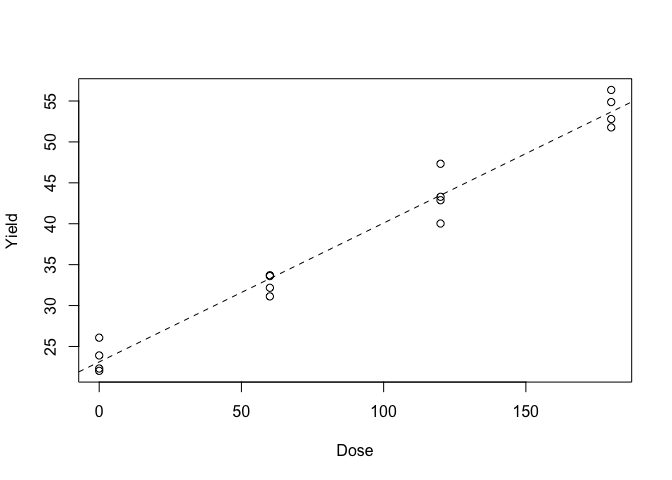
\includegraphics[width=0.9\linewidth]{_main_files/figure-latex/unnamed-chunk-109-1}

\begin{center}\rule{0.5\linewidth}{0.5pt}\end{center}

\hypertarget{further-readings-6}{%
\section{Further readings}\label{further-readings-6}}

\begin{enumerate}
\def\labelenumi{\arabic{enumi}.}
\tightlist
\item
  Maindonald J. Using R for Data Analysis and Graphics - Introduction, Examples and Commentary. (PDF, data sets and scripts are available at \href{https://cran.r-project.org/doc/contrib/usingR.pdff}{JM's homepage}.
\item
  Oscar Torres Reina, 2013. Introductio to RStudio (v. 1.3). \href{https://dss.princeton.edu/training/RStudio101.pdf}{This homepage}
\end{enumerate}


\end{document}
